\chapter{Results}


% Dire cosa vogliamo andare a guardare per capire come fare meglio, se possiamo fare meglio, quindi ci serve una metrica; poi cominci a giustificare i parametri che abbiamo messo nelle simulazioni; dai qualche indicazione operativa e poi inizi a commentare i risultati.

In this chapter, we will comment on the results obtained with the algorithms we described in the previous chapters: we will both analyze them individually and compare them with each other.

\section{Policy gradient methods}

We first implemented the ordinary policy gradient descent (\acrshort{pg}), using the formula for the gradient $\nabla_{\boldsymbol \theta} J_\pi (\boldsymbol \theta)$ in equation \eqref{eq:mygradJ}. Then, realizing how slow the convergence was, we decided to implement also the natural policy gradient algorithm (\acrshort{npg}), following equation \eqref{eq:mynatgradJ}. While reaching the same policy (the difference is in the order of $10^{-2}$), the \acrshort{npg} reaches convergence way faster than the \acrshort{pg} algorithm, as we can see from the right panel of \autoref{fig:times}. The figure reports the convergence times of the two algorithms, for different numbers of initially disconnected substations. From the left panel, which reports the same times but in logarithmic scale, we can see that both the two curves are exponentials, with approximately the same rate, but the \acrshort{npg} one has an initial value about $10^{-2}$ times smaller than the \acrshort{pg} one, which considerably reduces the computation time. For example, with $13$ initially disconnected substations, the convergence of the \acrshort{pg} took $20$ hours, while the convergence of the \acrshort{npg} took $17$ minutes.
% ab^x, cd^x -> log(ab^x), log(cd^x) -> log(a)+xlog(b), log(c)+xlog(d) -> log(b) = log(d), log(a) != log(c)

\begin{figure}[t]
    \centering
    \mbox{
        \hspace*{-15pt}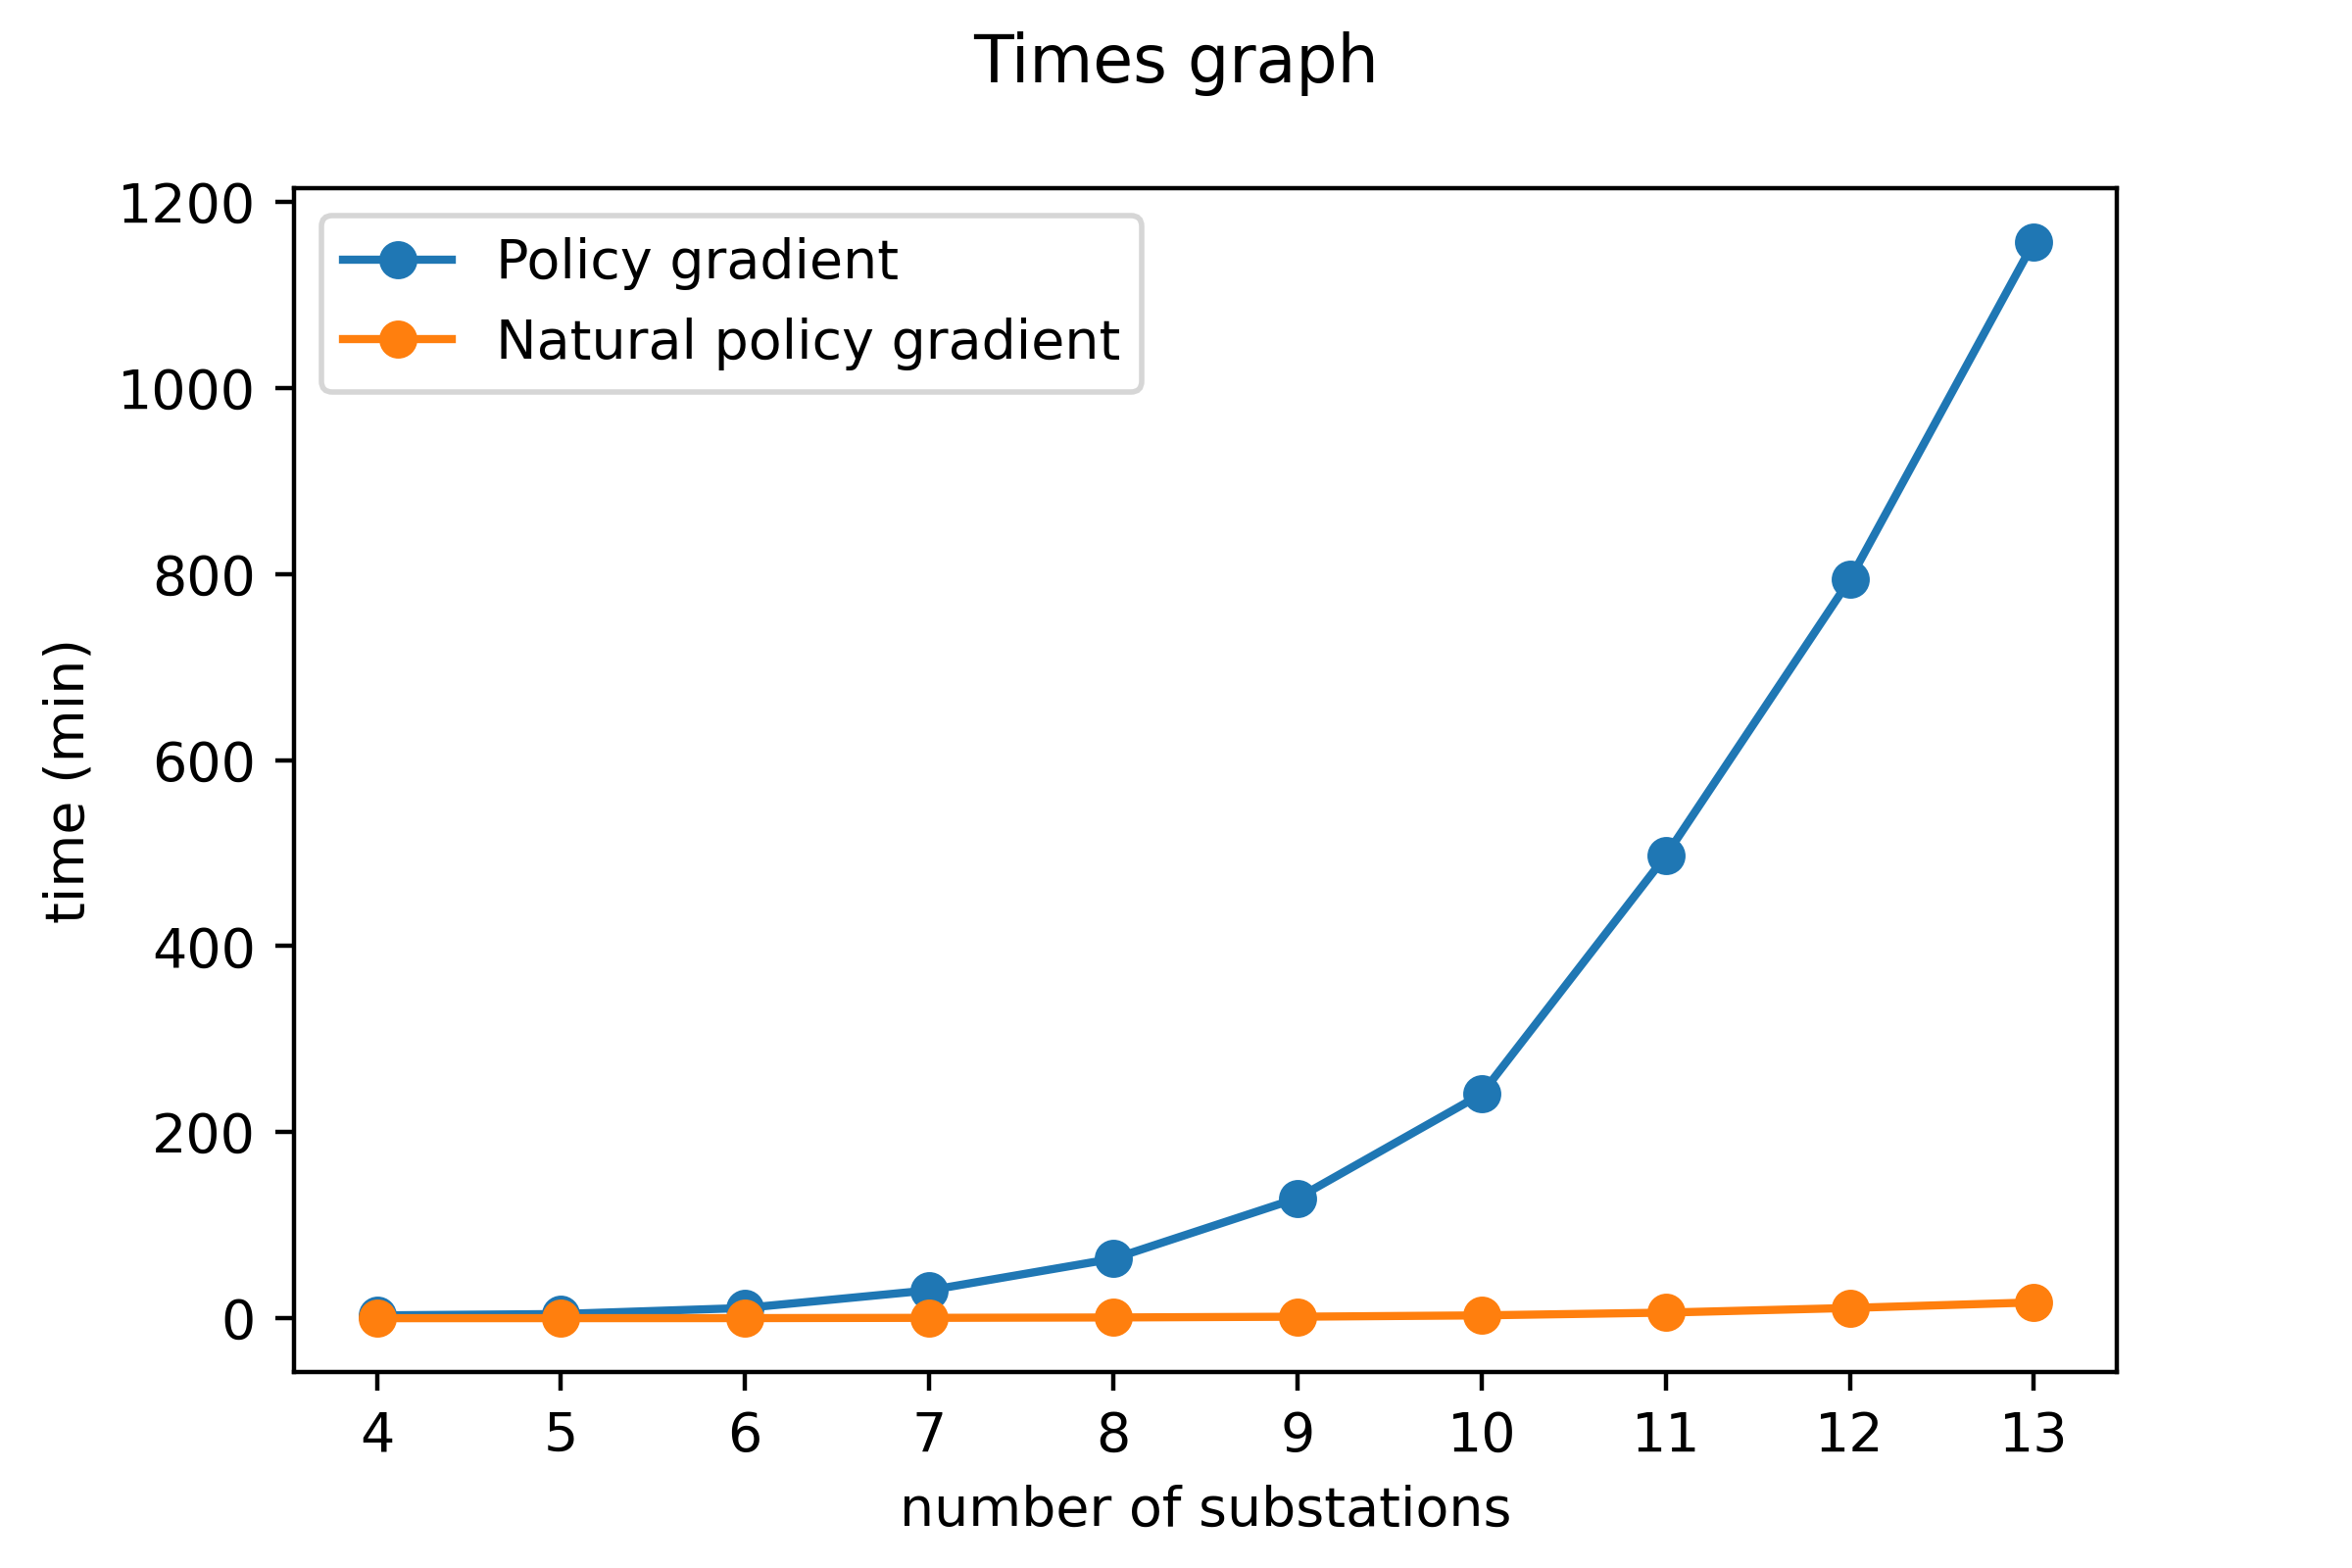
\includegraphics[scale=0.52]{chapters/figures/times_graph.png}
        \hspace*{-5pt}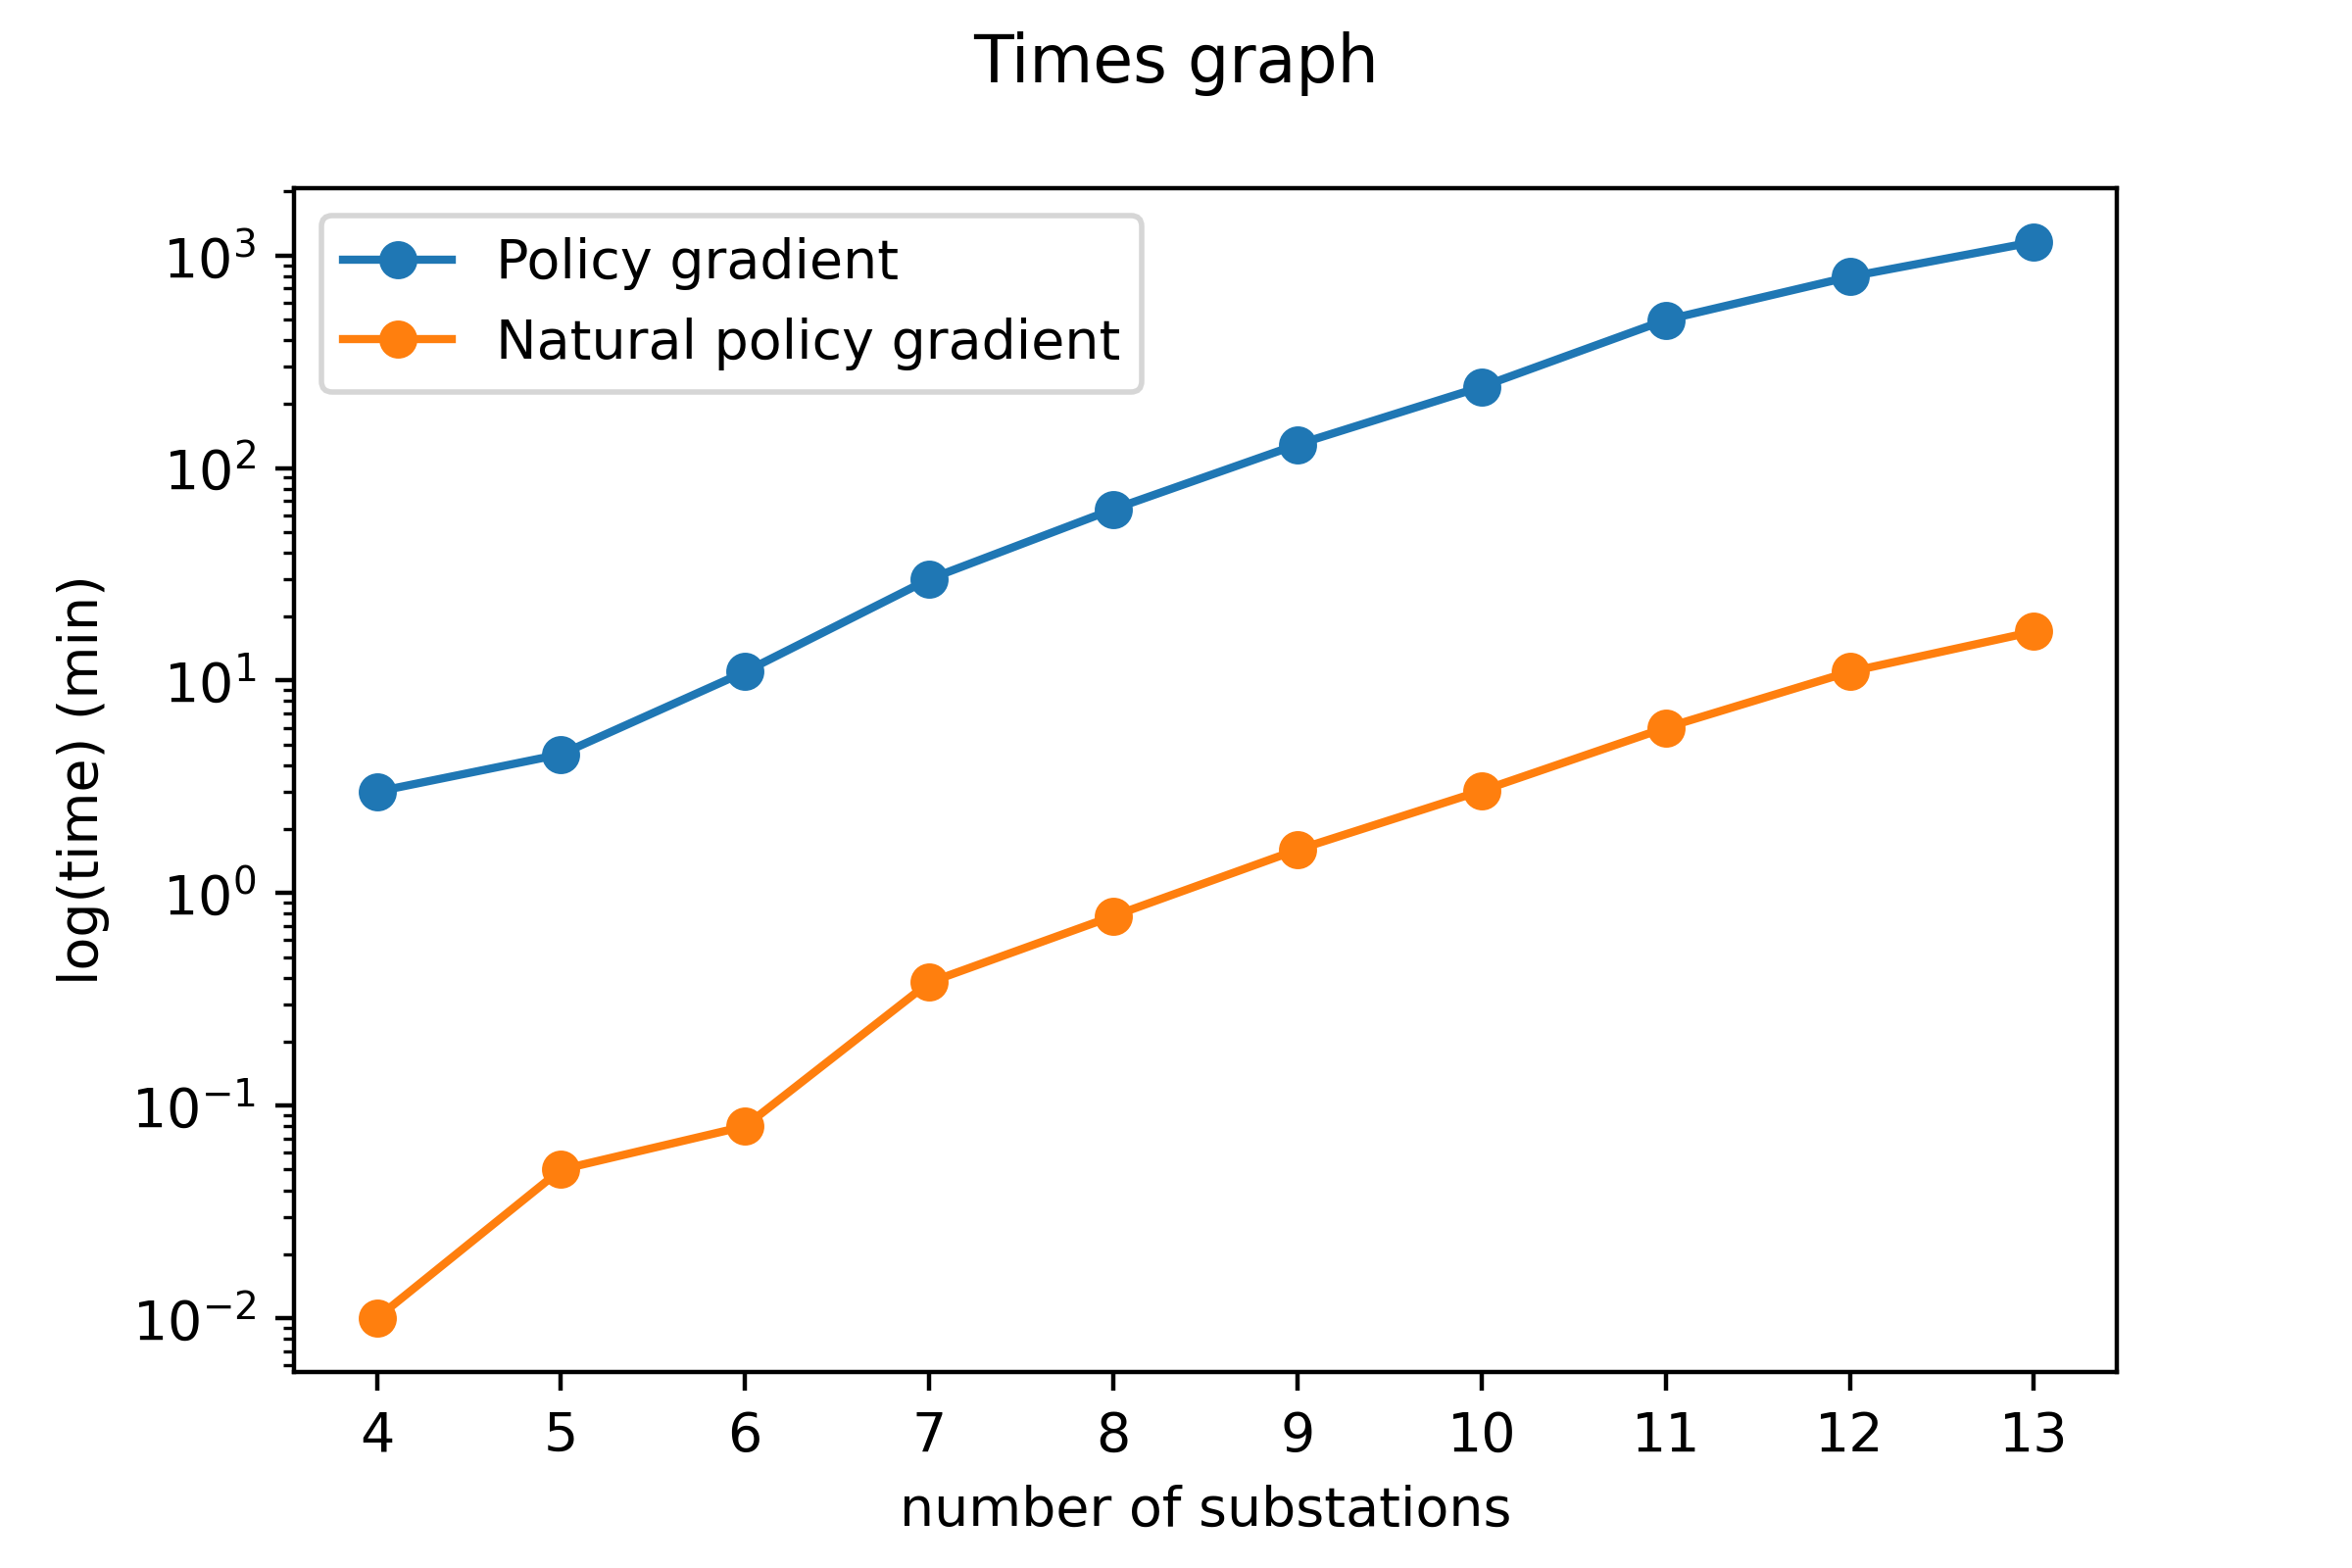
\includegraphics[scale=0.52]{chapters/figures/times_graph_log.png}
    }
    \caption{Comparison of the convergence times of \acrshort{pg} and \acrshort{npg} algorithms for different numbers of initially disconnected substations. The second figure shows the same times but in logarithmic scale.}
    \label{fig:times}
\end{figure}

These two algorithms find a policy that is not completely deterministic: in fact, some states have a stochastic policy over their possible actions. This means that we are on a side of the simplex which represents the policy space, and not in a corner. However, when, given a fault, we followed the actions dictated by the policy, we ended up only in states with a deterministic choice of the action to be performed. In particular, an interesting thing to notice is that, in the initial state, the policy always prescribes to go to the substation in the middle, like the bisection algorithm. Then, for subsequent substations, the two policies begin to differ, giving remarkably different results, as we will see later.

The first thing to look at in a policy gradient algorithm is whether the gradient descent reached convergence. The first, immediate, check is to see if the error is decreasing. We checked this both for the \acrshort{pg} algorithm and for the \acrshort{npg} algorithm, and both of them were decreasing, as we can see from the plots of \autoref{fig:errors}. In the left panel we have the errors of the ordinary policy gradient with both axes in logarithmic scale. Since we have two straight segments, the errors follow two different decreasing power laws; until just before $10^2$ steps, the errors decrease slowly, while afterwards they decrease faster.
%; which is consistent with the very slow convergence of the algorithm.
Instead, in the right panel we can see the errors of the natural policy gradient: here we have two lines with different slopes, which indicates that initially the errors decrease faster, while after about $100$ steps they start decreasing according to an exponential with a lower rate.

\begin{figure}[t]
    \centering
    \mbox{
        \hspace*{-10pt}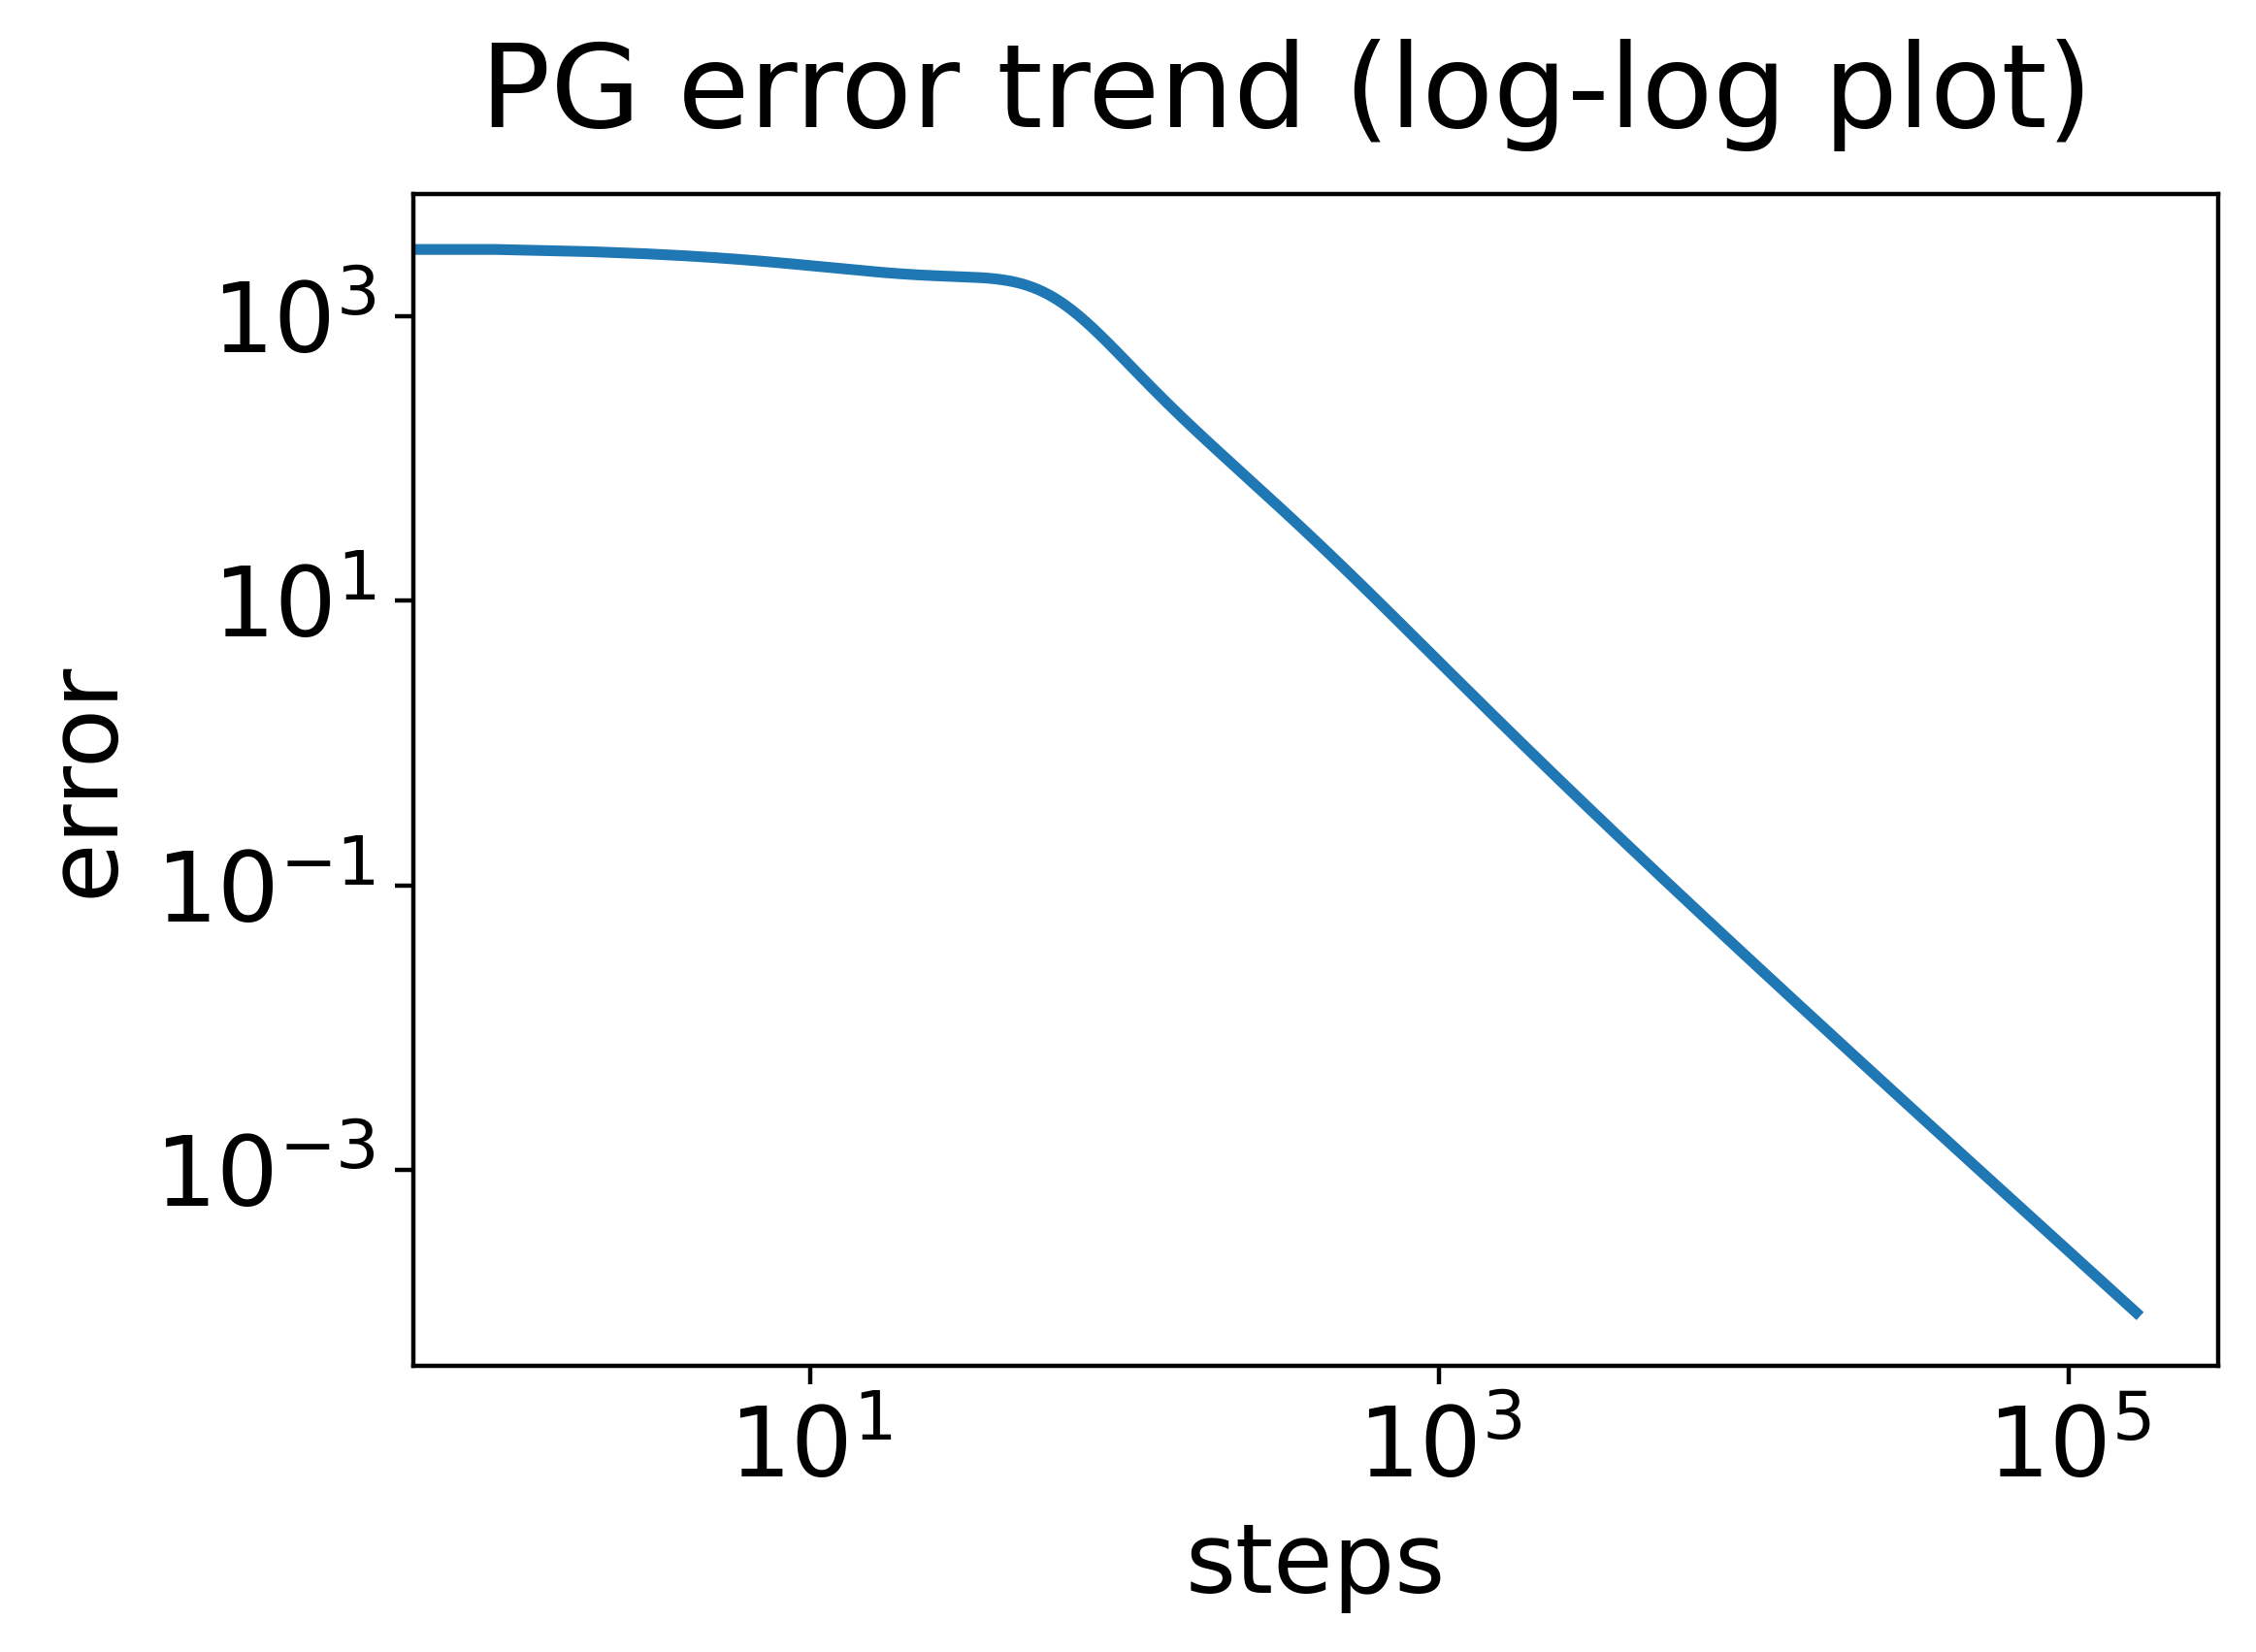
\includegraphics[scale=0.52]{chapters/figures/errors_log_log_PG.png}
        \hspace*{-5pt}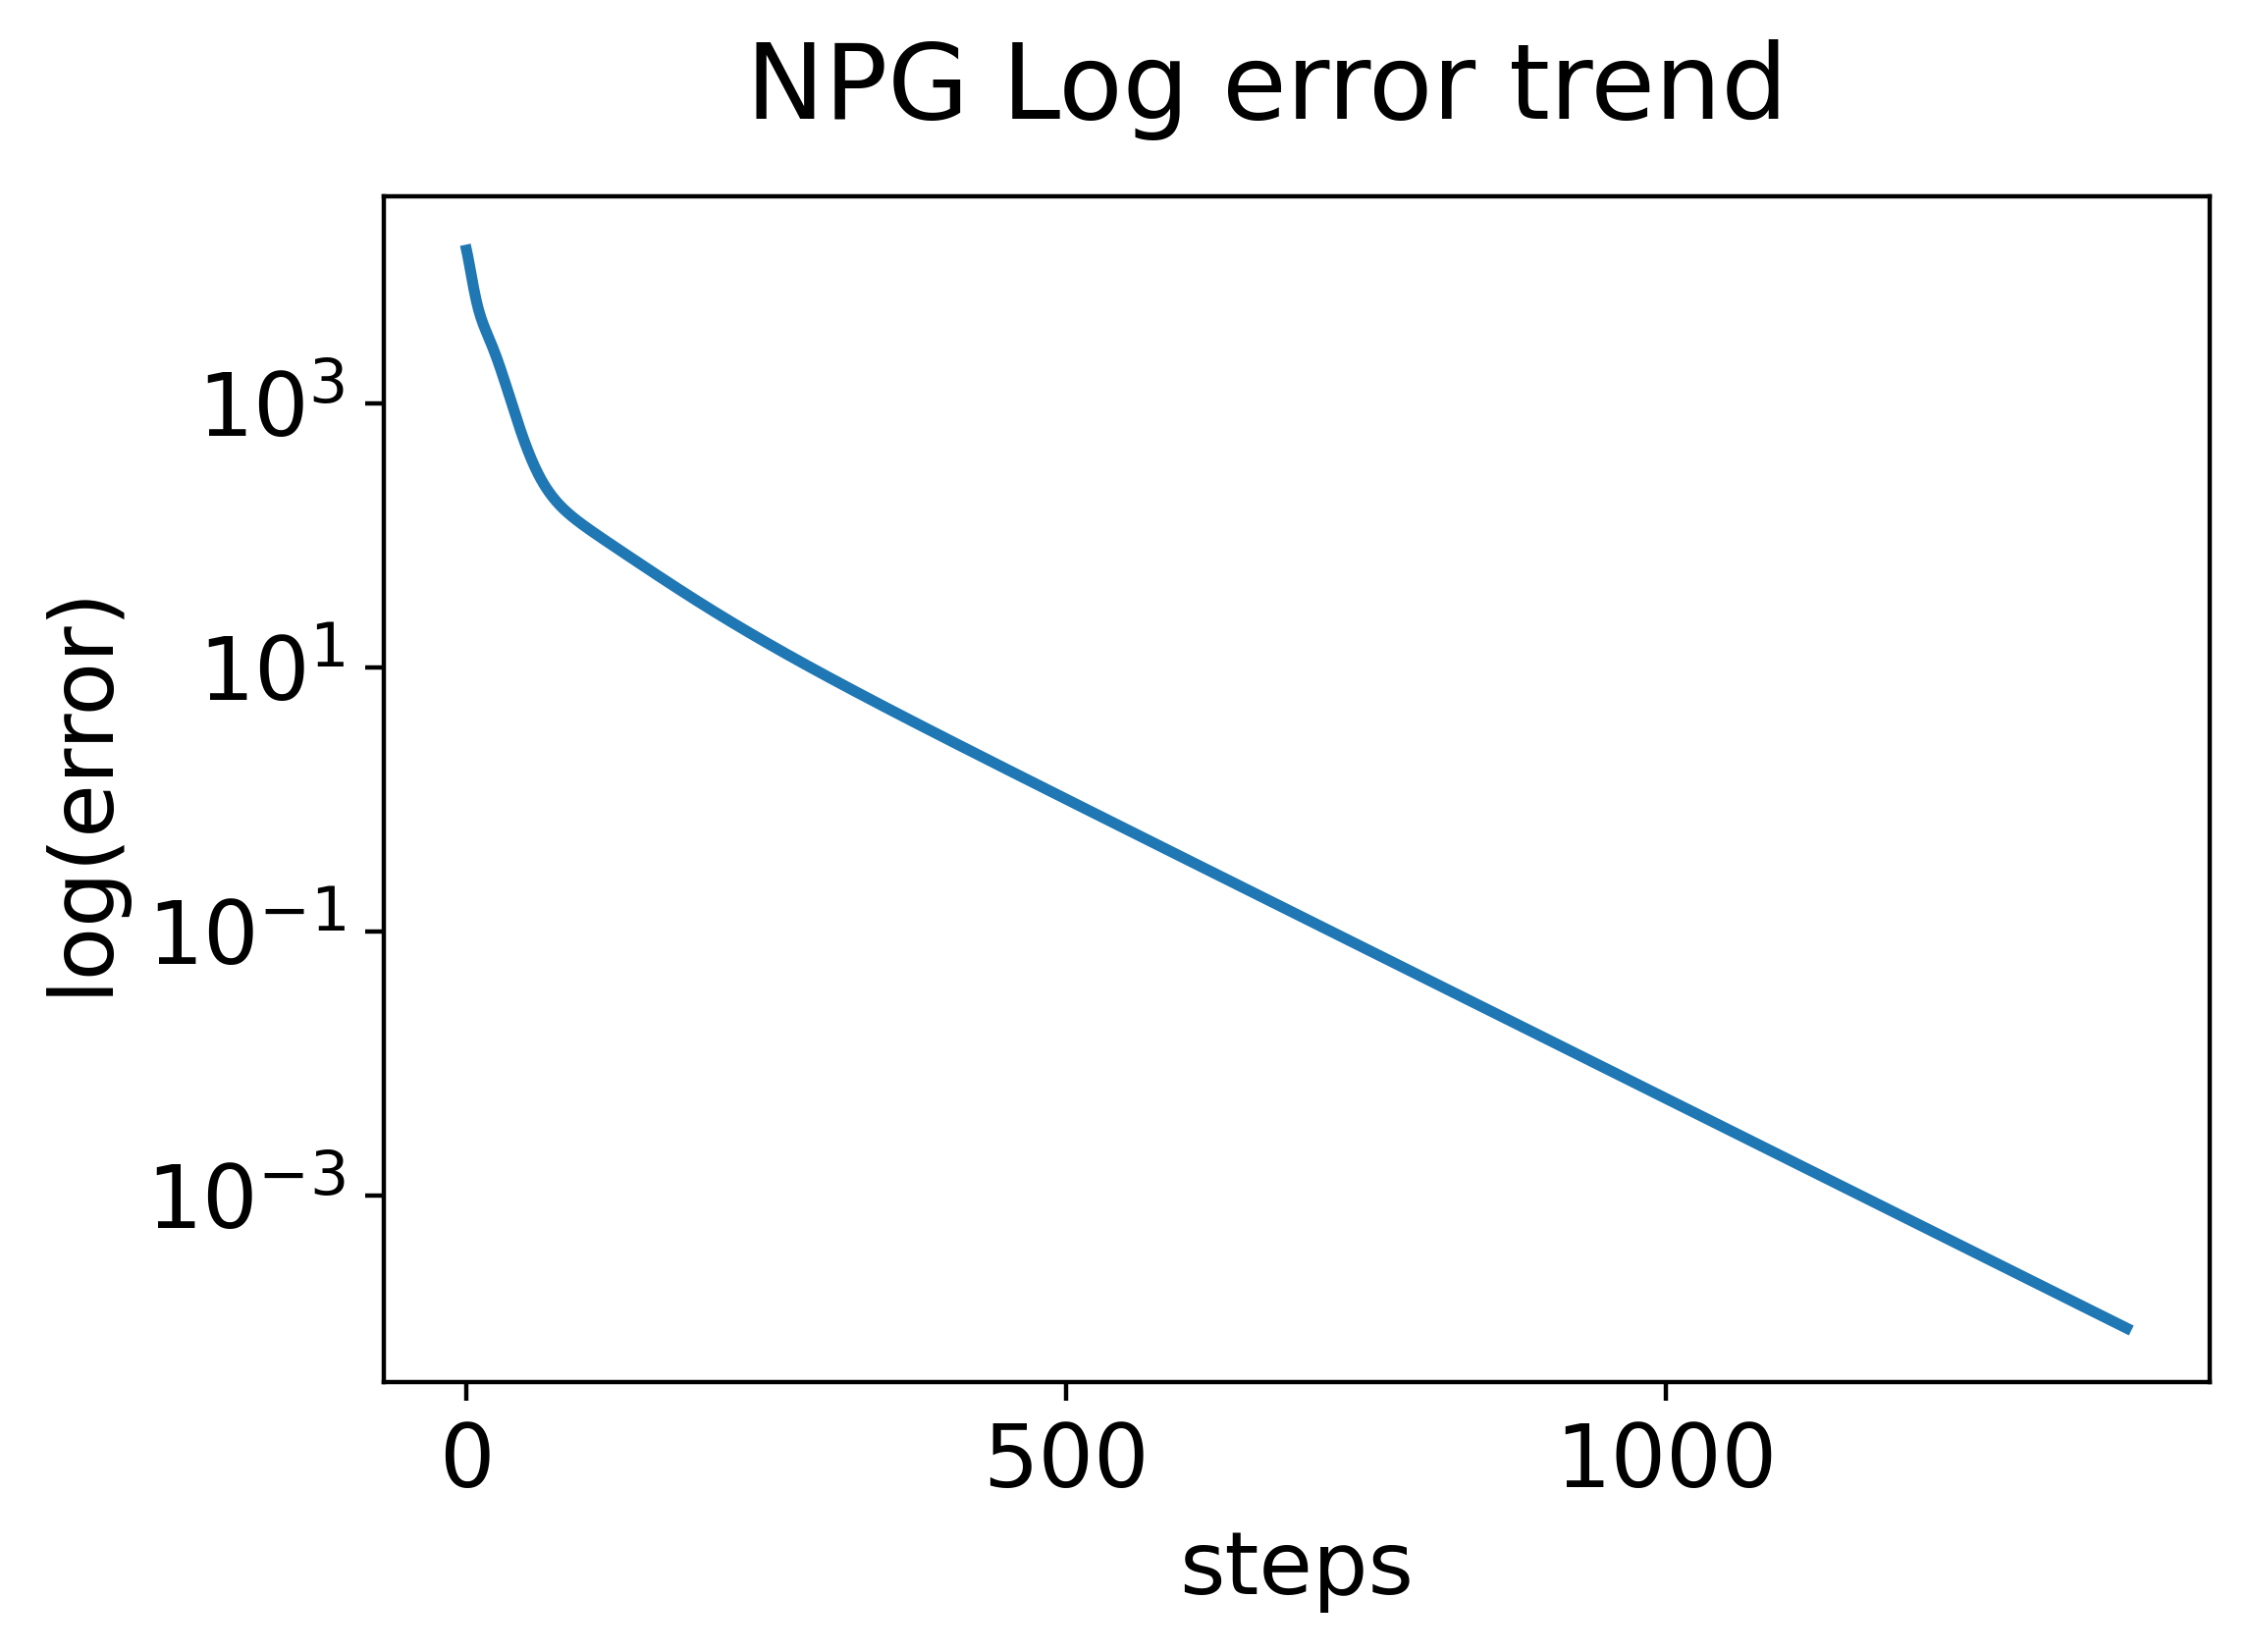
\includegraphics[scale=0.52]{chapters/figures/errors_log_NPG.png}
    }
    \caption{On the left there are the \acrshort{pg} errors, while on the right the \acrshort{npg} ones, both for $5$ initially disconnected substations. They are both decreasing, so the gradient descent is following a minimum, as we want it to do.}
    \label{fig:errors}
\end{figure}

However, this is not enough to say that the algorithm converged, this is a mere indicator that the gradient descent is indeed following the gradient and moving towards a minimum. Thus, what we did next was to examine the trajectories of the parameters $\boldsymbol \theta$ in the parameters space and the trajectories of the policies $\pi_{\boldsymbol \theta}$ in the policy space. In \autoref{fig:sequence-theta-pg} and \autoref{fig:sequence-policies-pg} we can see these two quantities for the \acrshort{pg}, where we selected a specific episode with $5$ initially disconnected substation and the fault among the second and the third substation. In \autoref{fig:sequence-theta-npg} and \autoref{fig:sequence-policies-npg} we can see these two quantities for the \acrshort{npg} for the same exact episode. In each panel, the current state is reported in the title, and the plot represents the trajectory of the parameters $\boldsymbol \theta$ or the policy $\pi_{\boldsymbol \theta}$ for that specific state. Thus, we can see the parameters or the value of the policy for each specific action that can be taken in that state. The numbers in the states and in the labels represent the codes of the substations, and the faulty cable is indicated with the codes of the two substations at its ends. The subsequent panels represent the next states in which we end up taking the action suggested by the policy in the previous panel.

\begin{figure}[!htp]
    \centering
    \begin{tabular}{cc}
        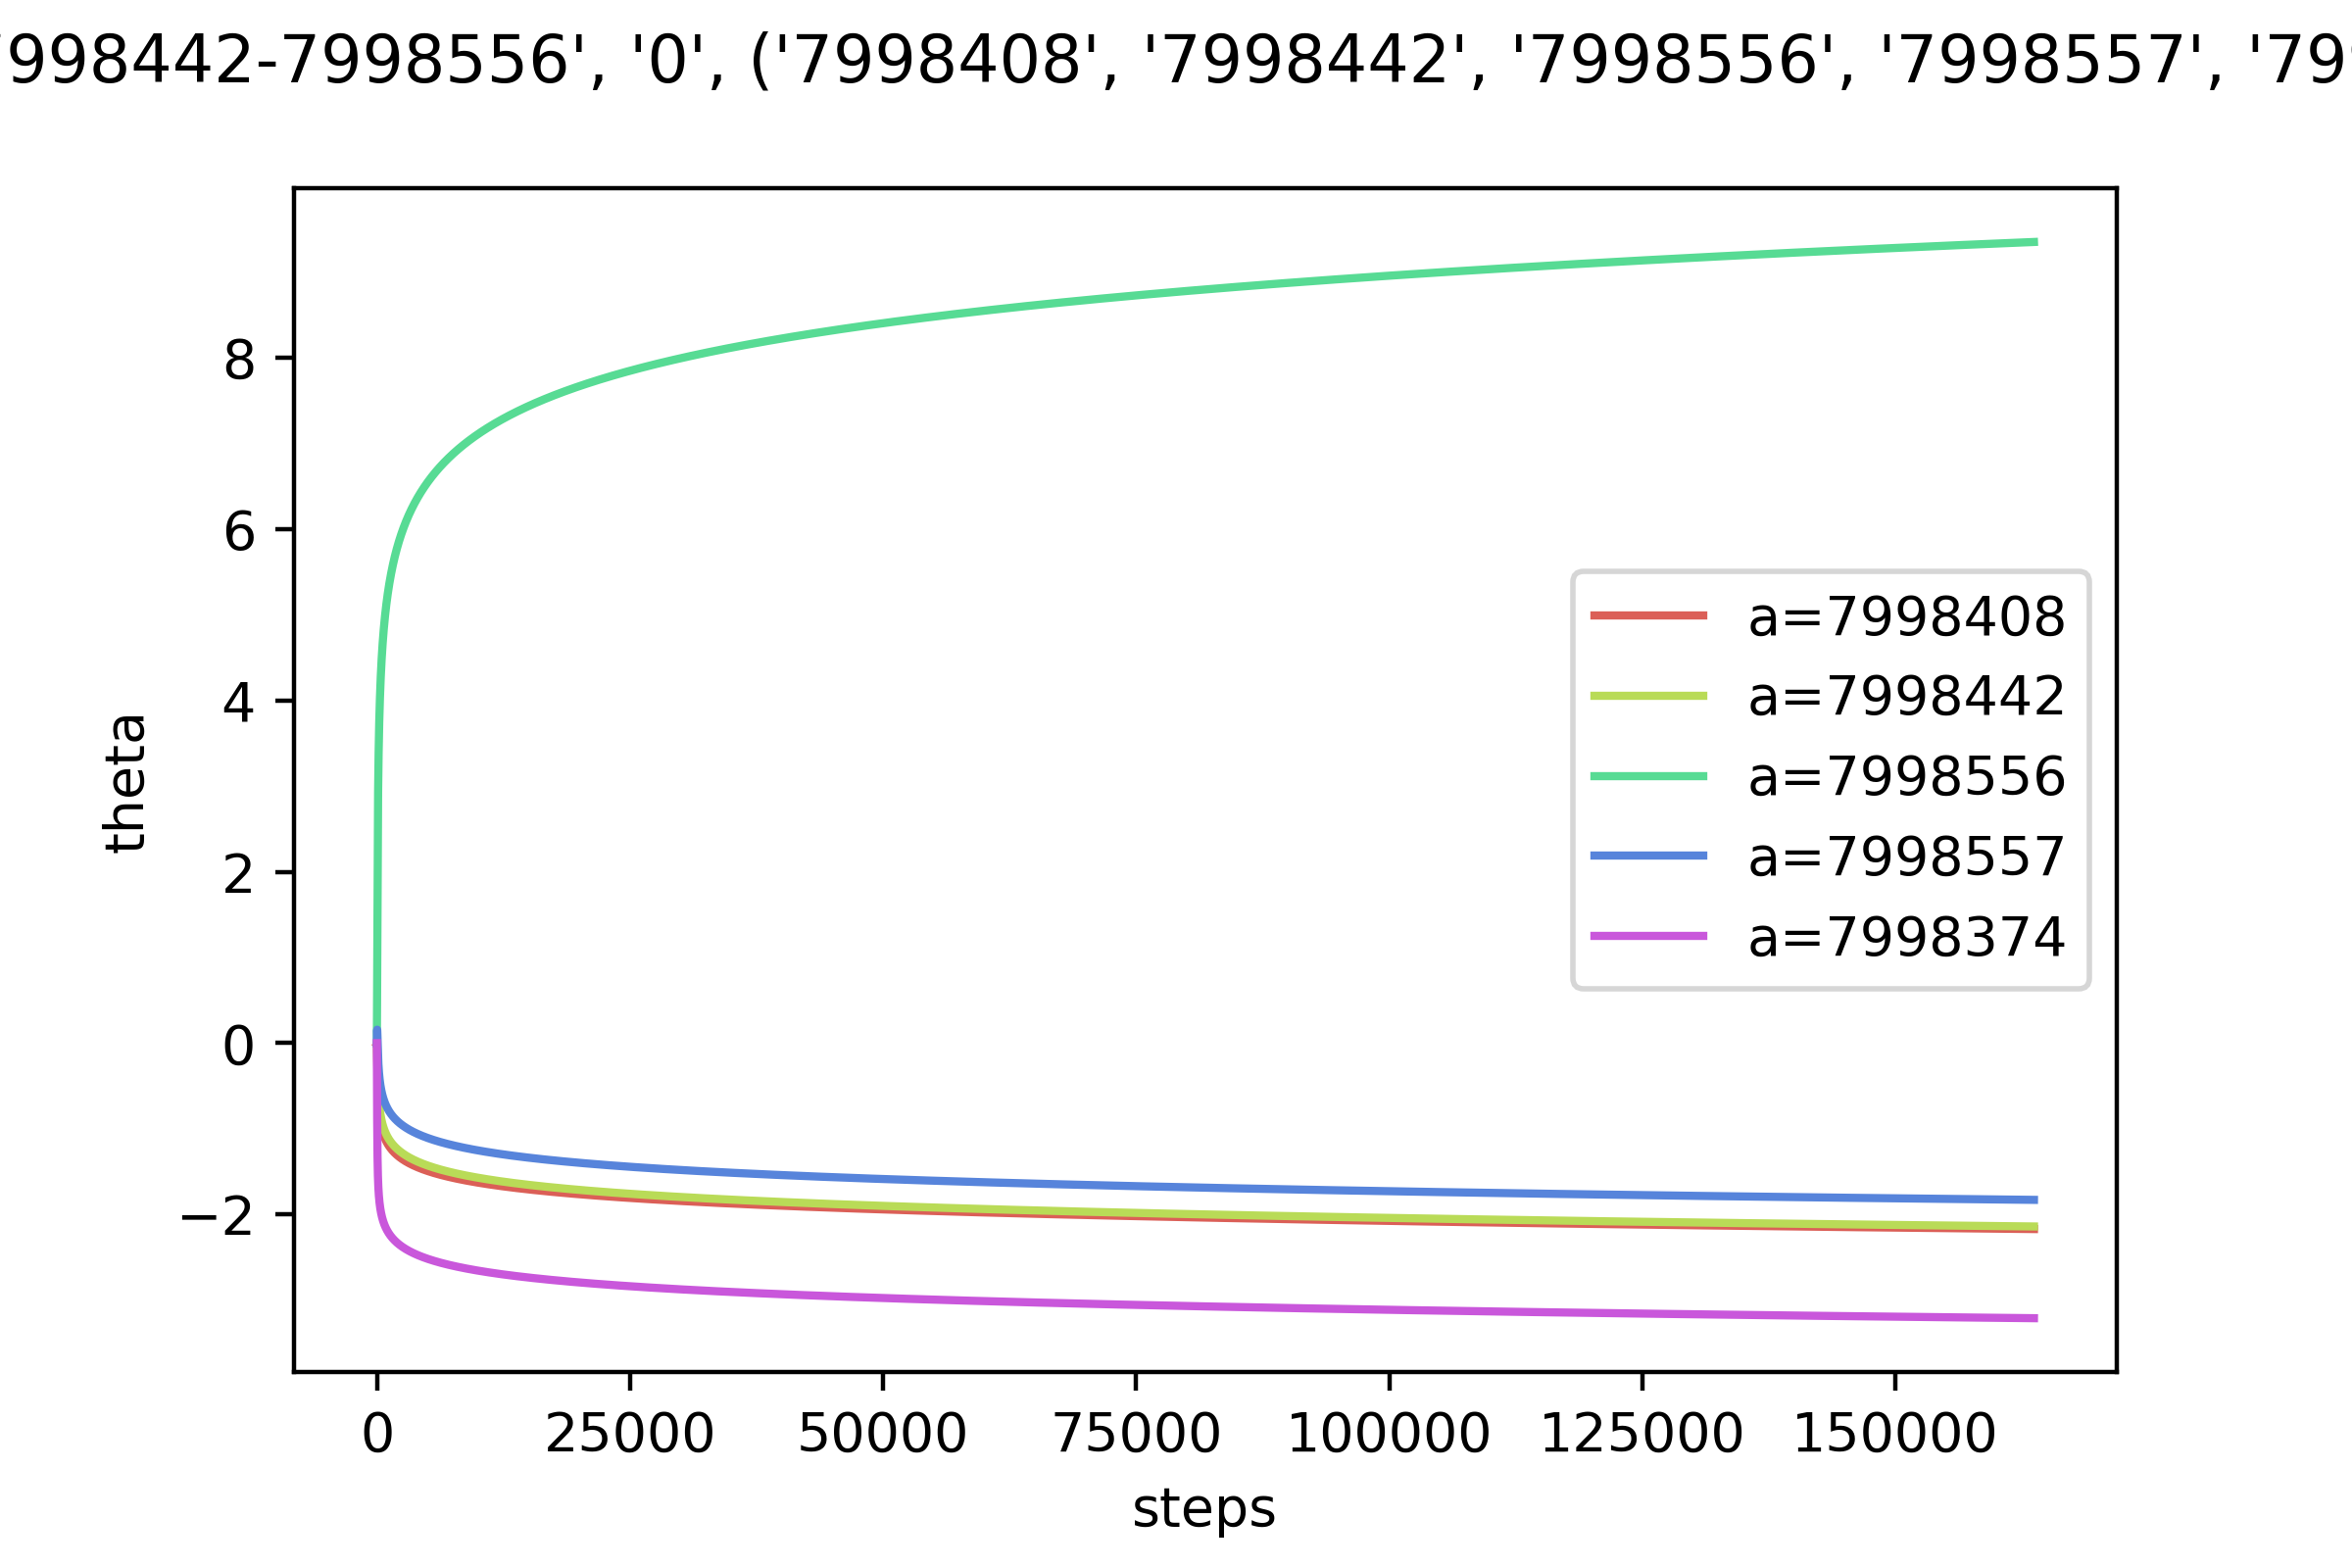
\includegraphics[scale=0.36,valign=b]{chapters/figures/theta_PG_state_0.png} &
        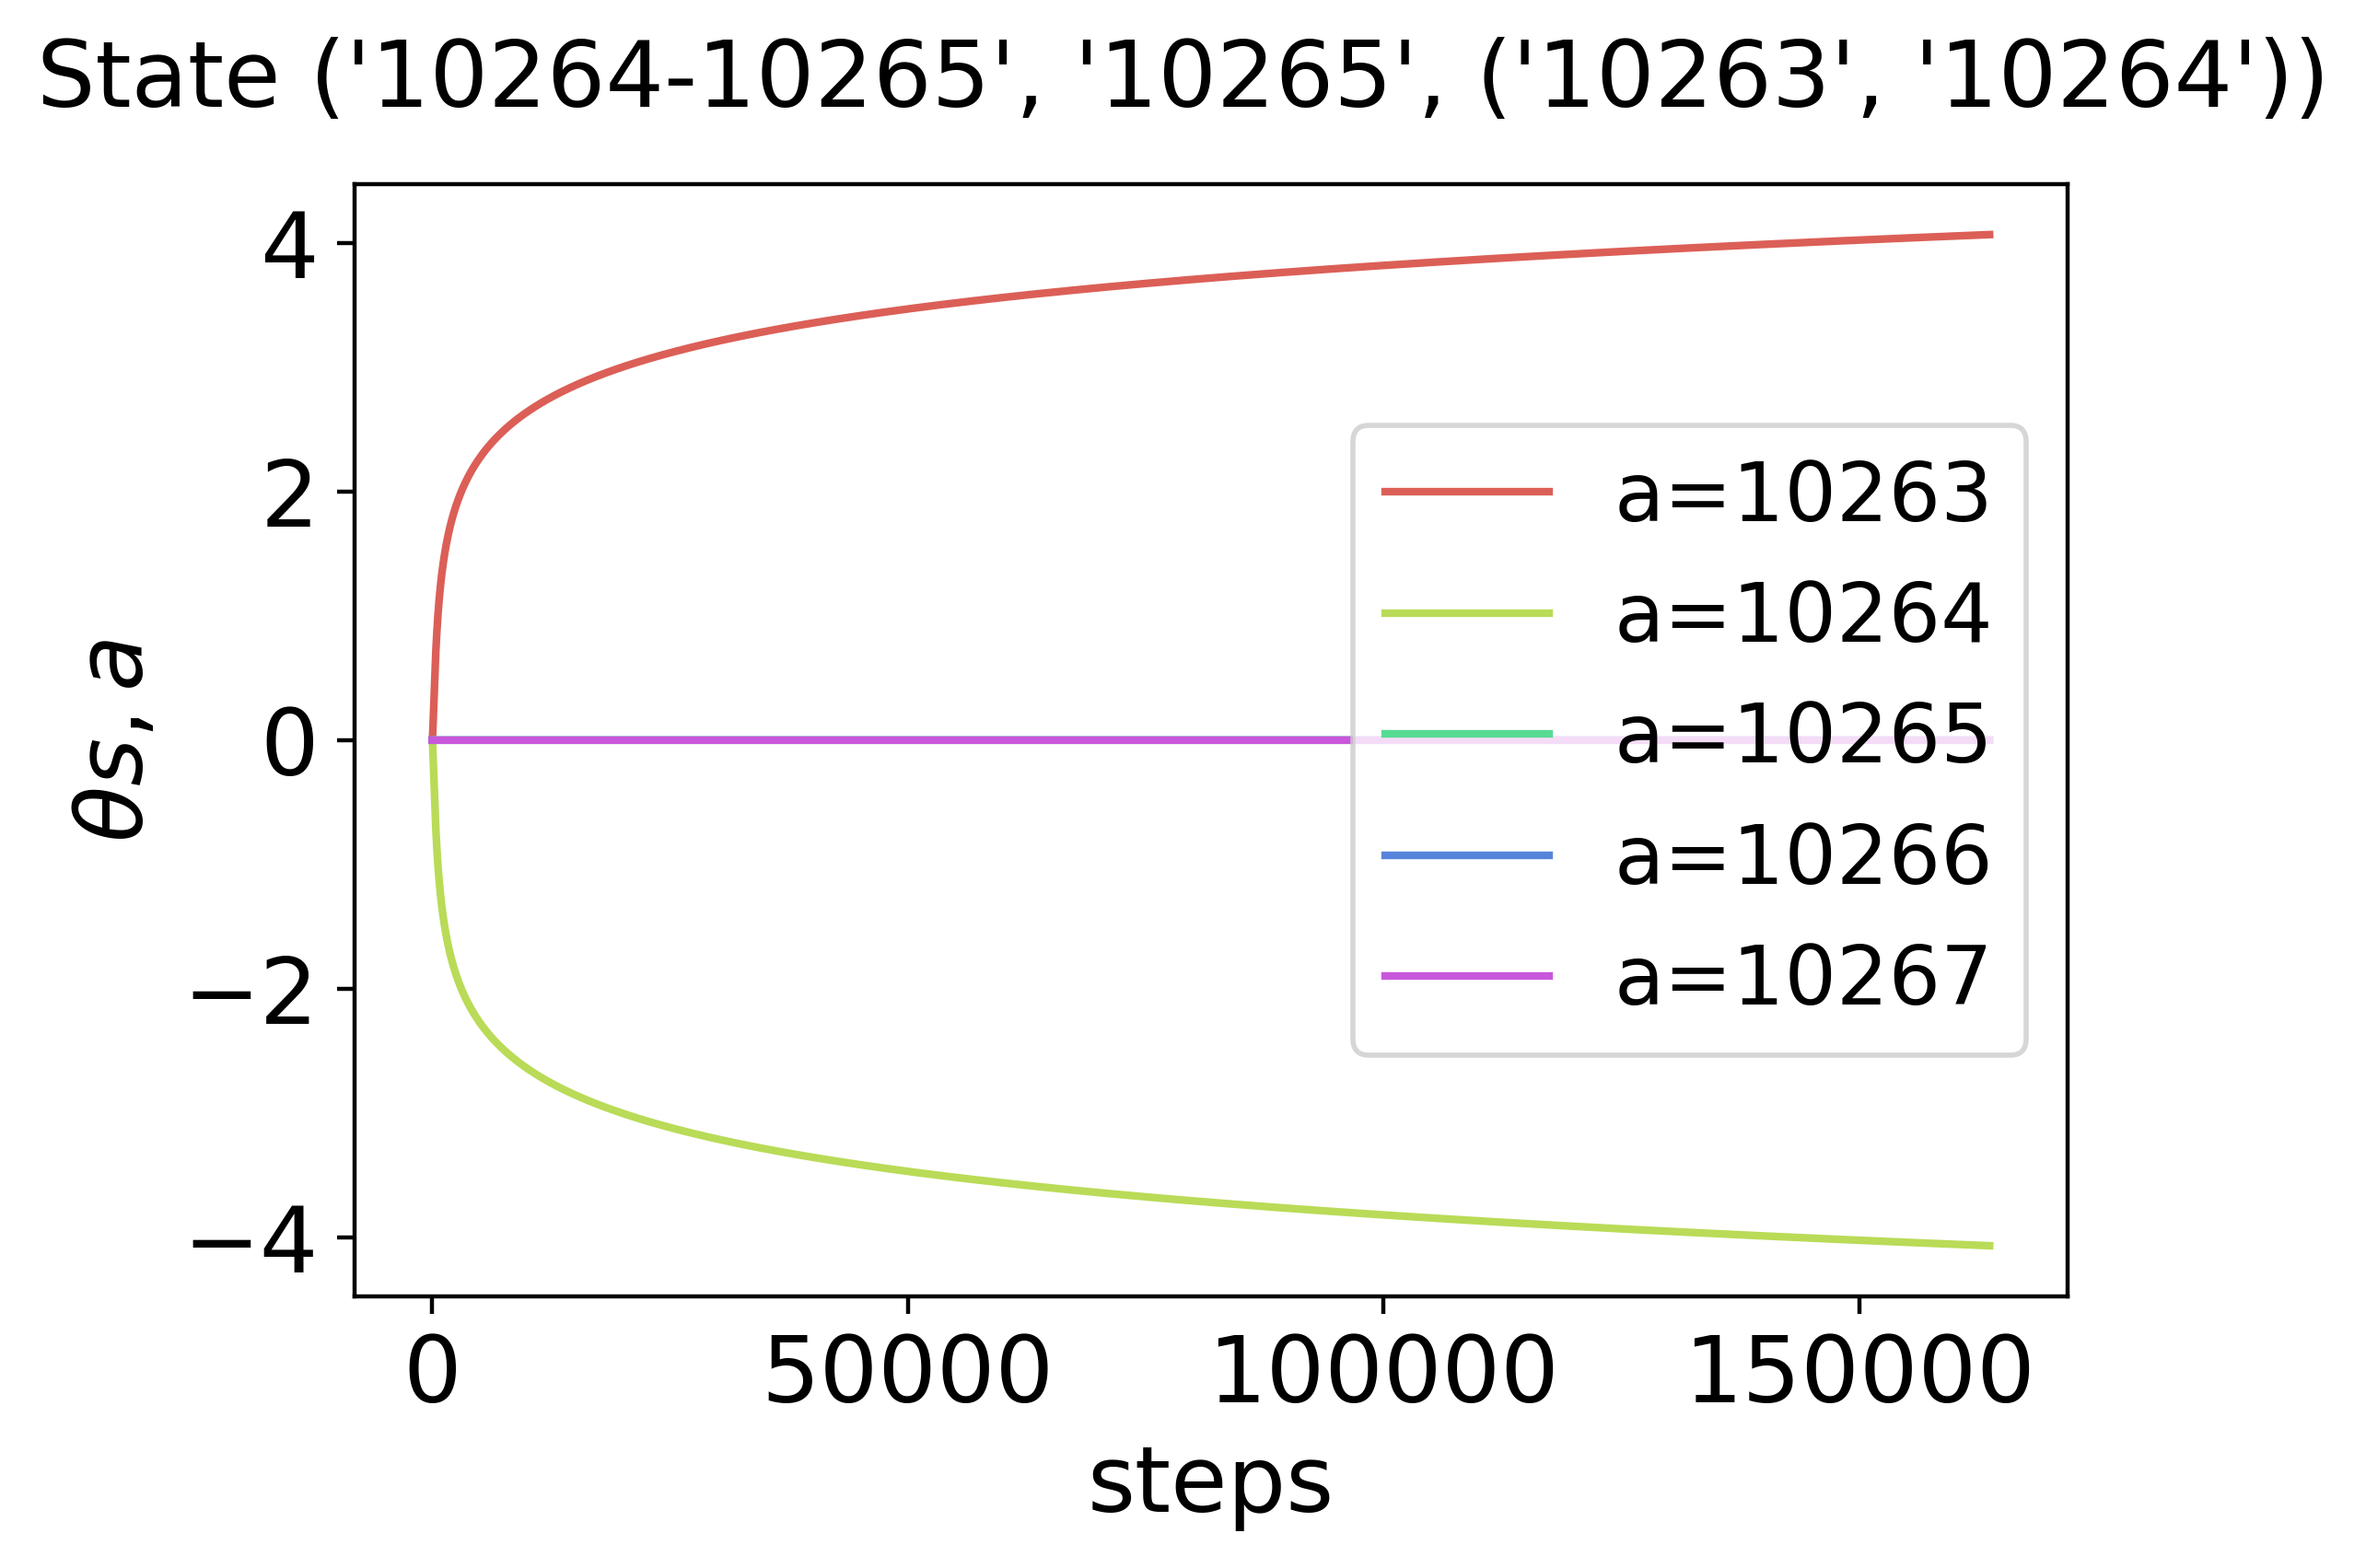
\includegraphics[scale=0.36,valign=b]{chapters/figures/theta_PG_state_1.png} \\
        \hspace*{-10pt}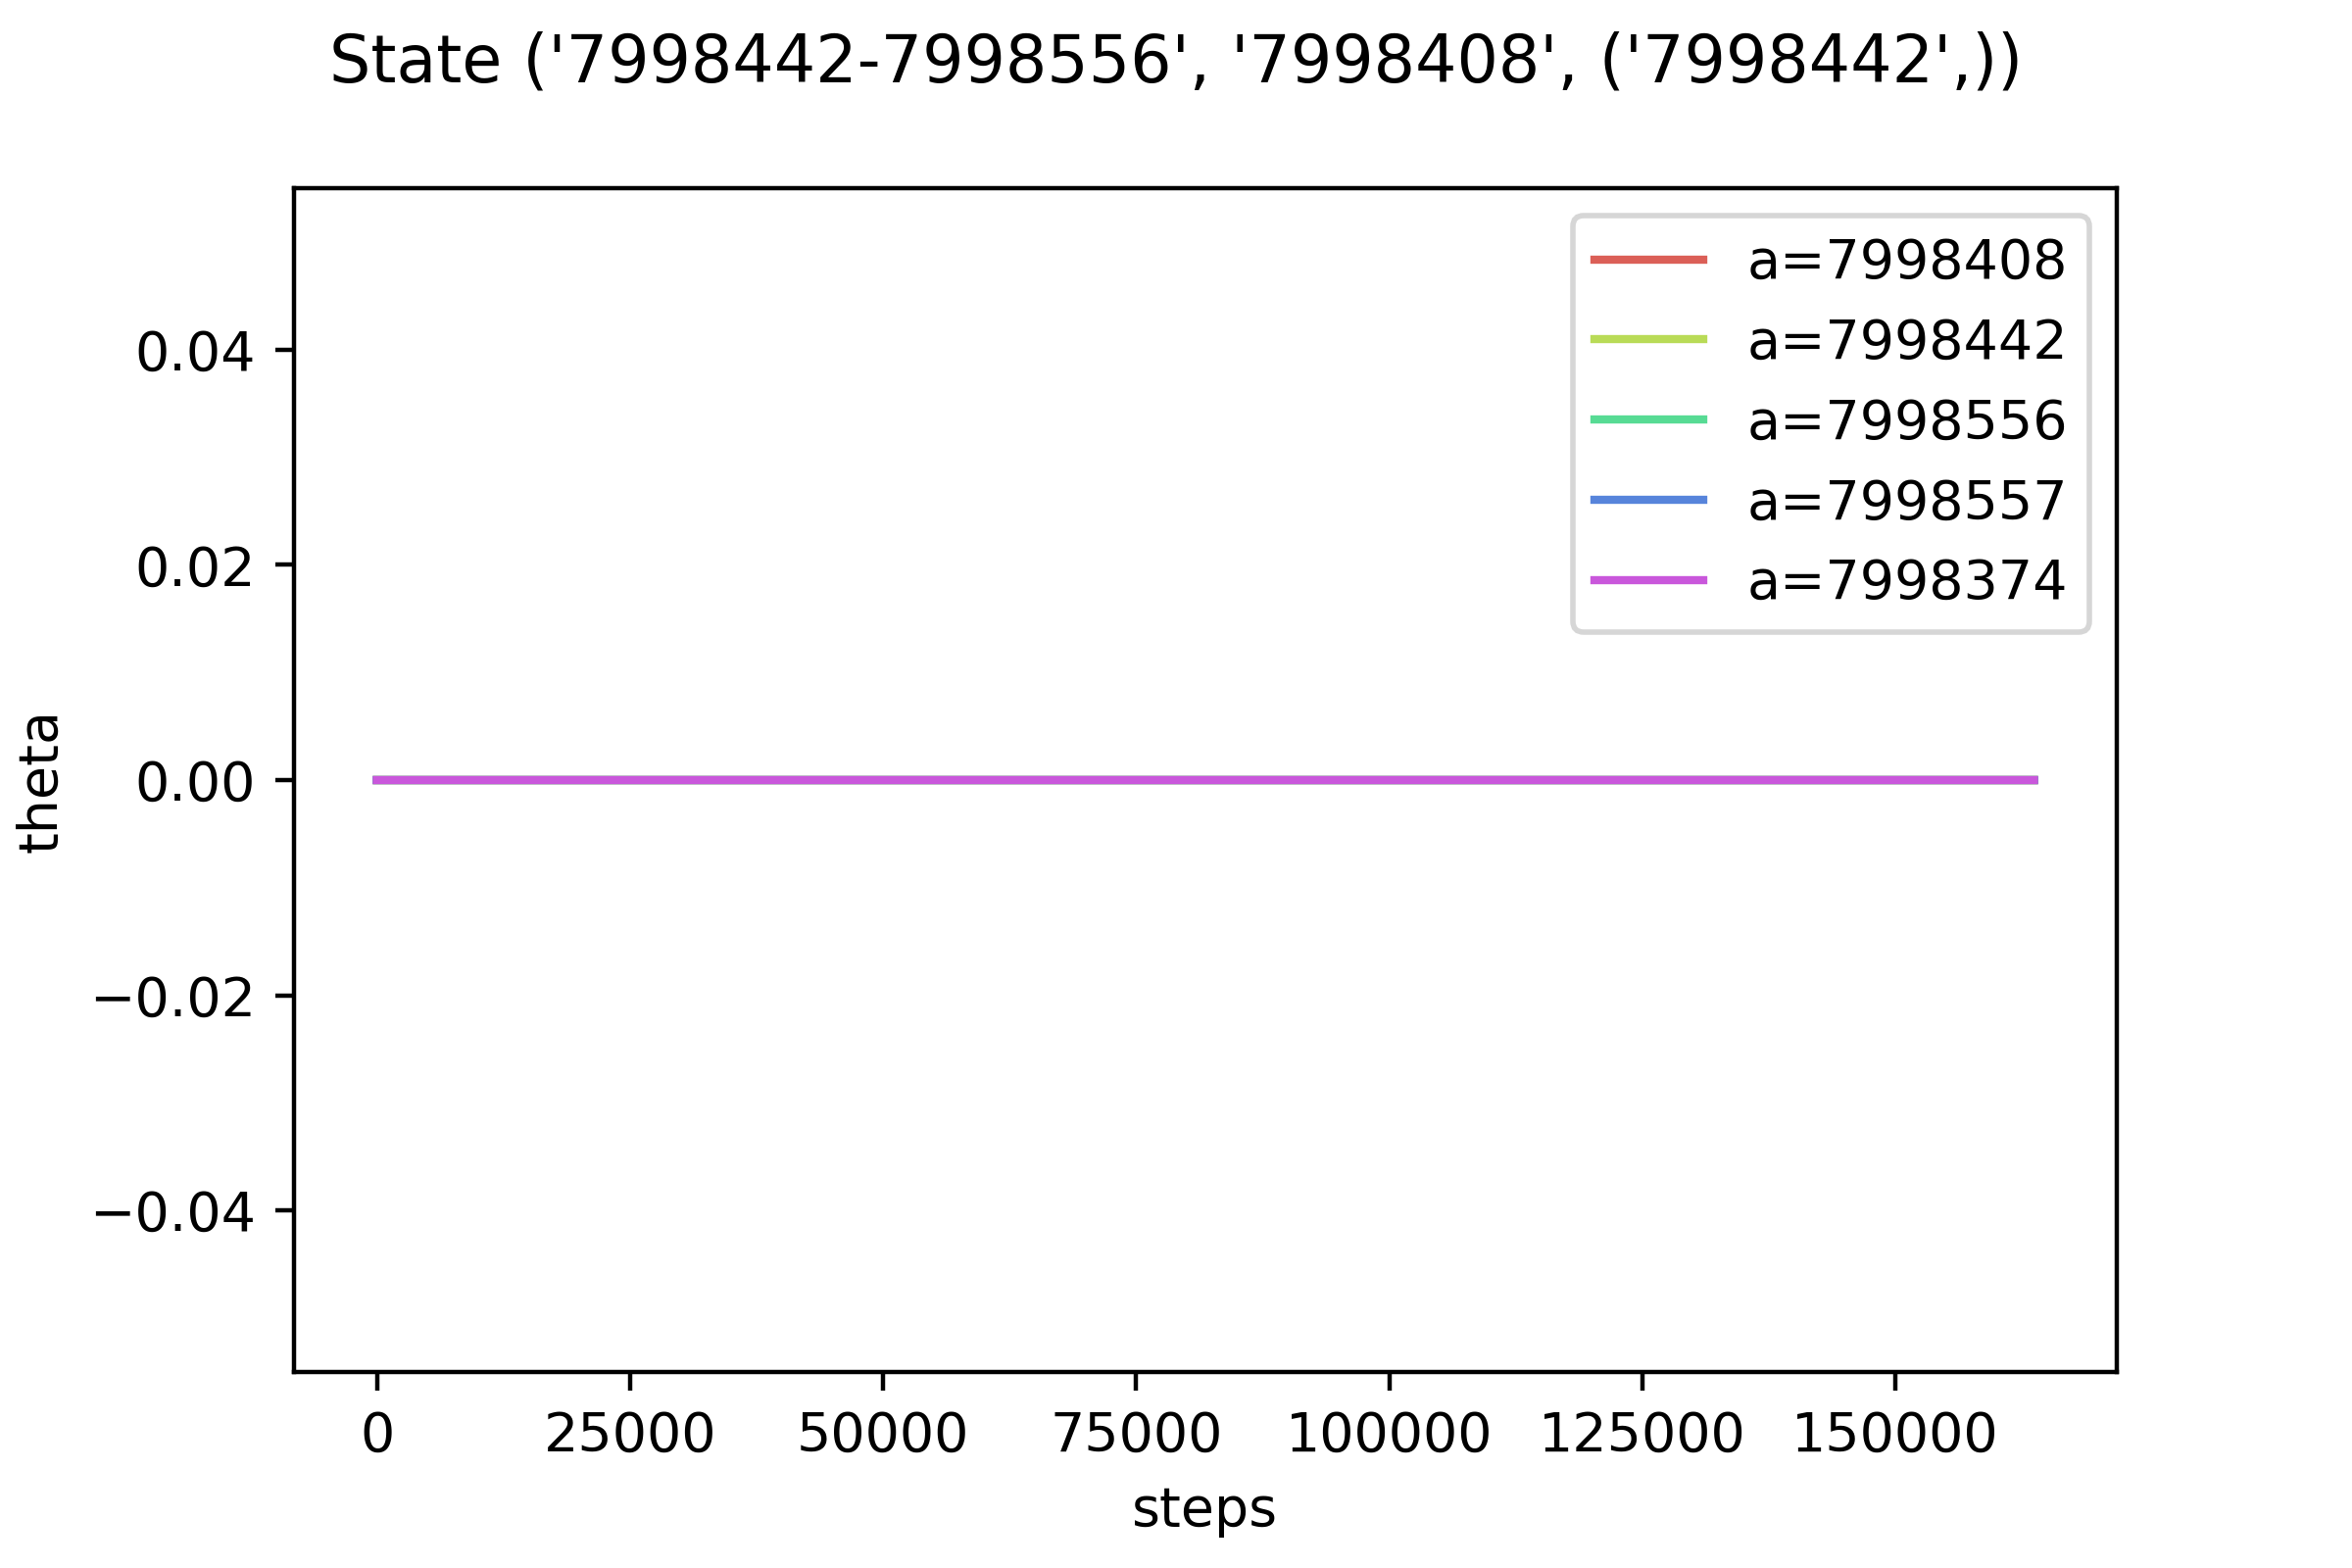
\includegraphics[scale=0.36,valign=b]{chapters/figures/theta_PG_state_2.png} &
        \hspace*{-28pt}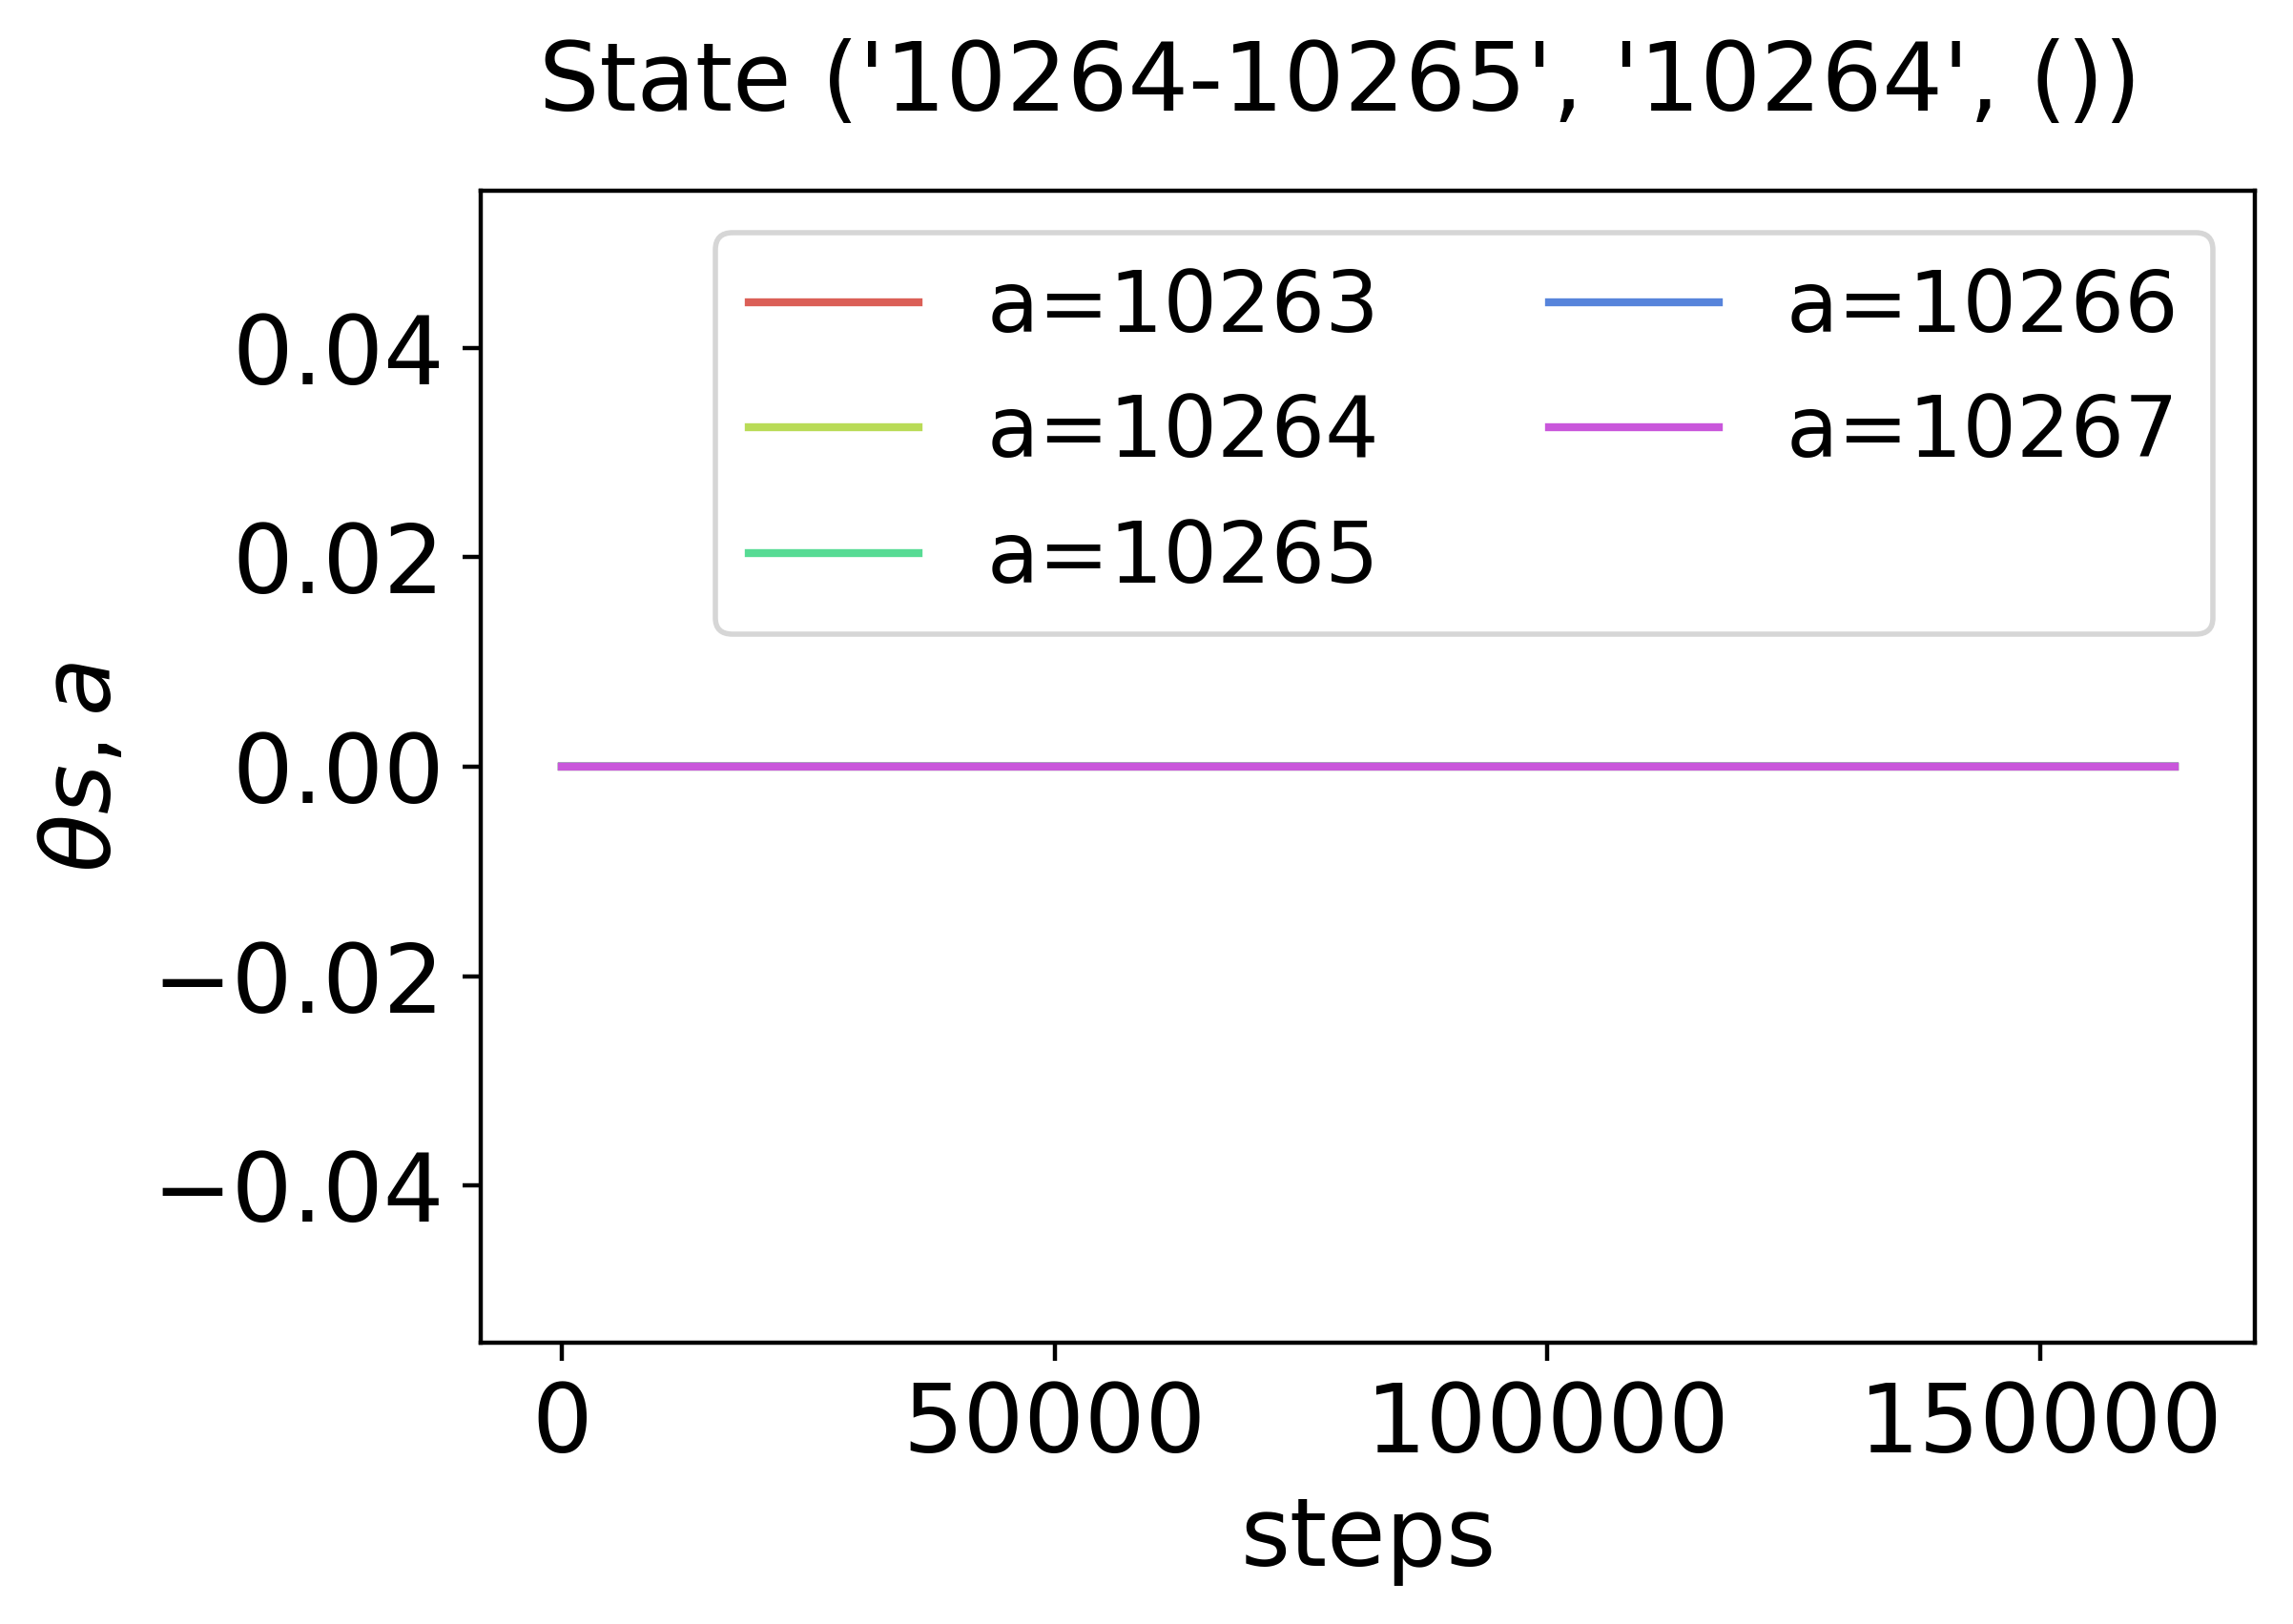
\includegraphics[scale=0.36,valign=b]{chapters/figures/theta_PG_state_3.png}
    \end{tabular}
    \caption{\small Trajectories of the parameters $\boldsymbol \theta$ in the parameters space for \acrshort{pg}, for a specific episode (which starts in the top-left corner and goes from left to right, line by line) with $5$ initially disconnected substation.}
    \label{fig:sequence-theta-pg}
\end{figure}

\begin{figure}[!htp]
    \centering
    \begin{tabular}{cc}
        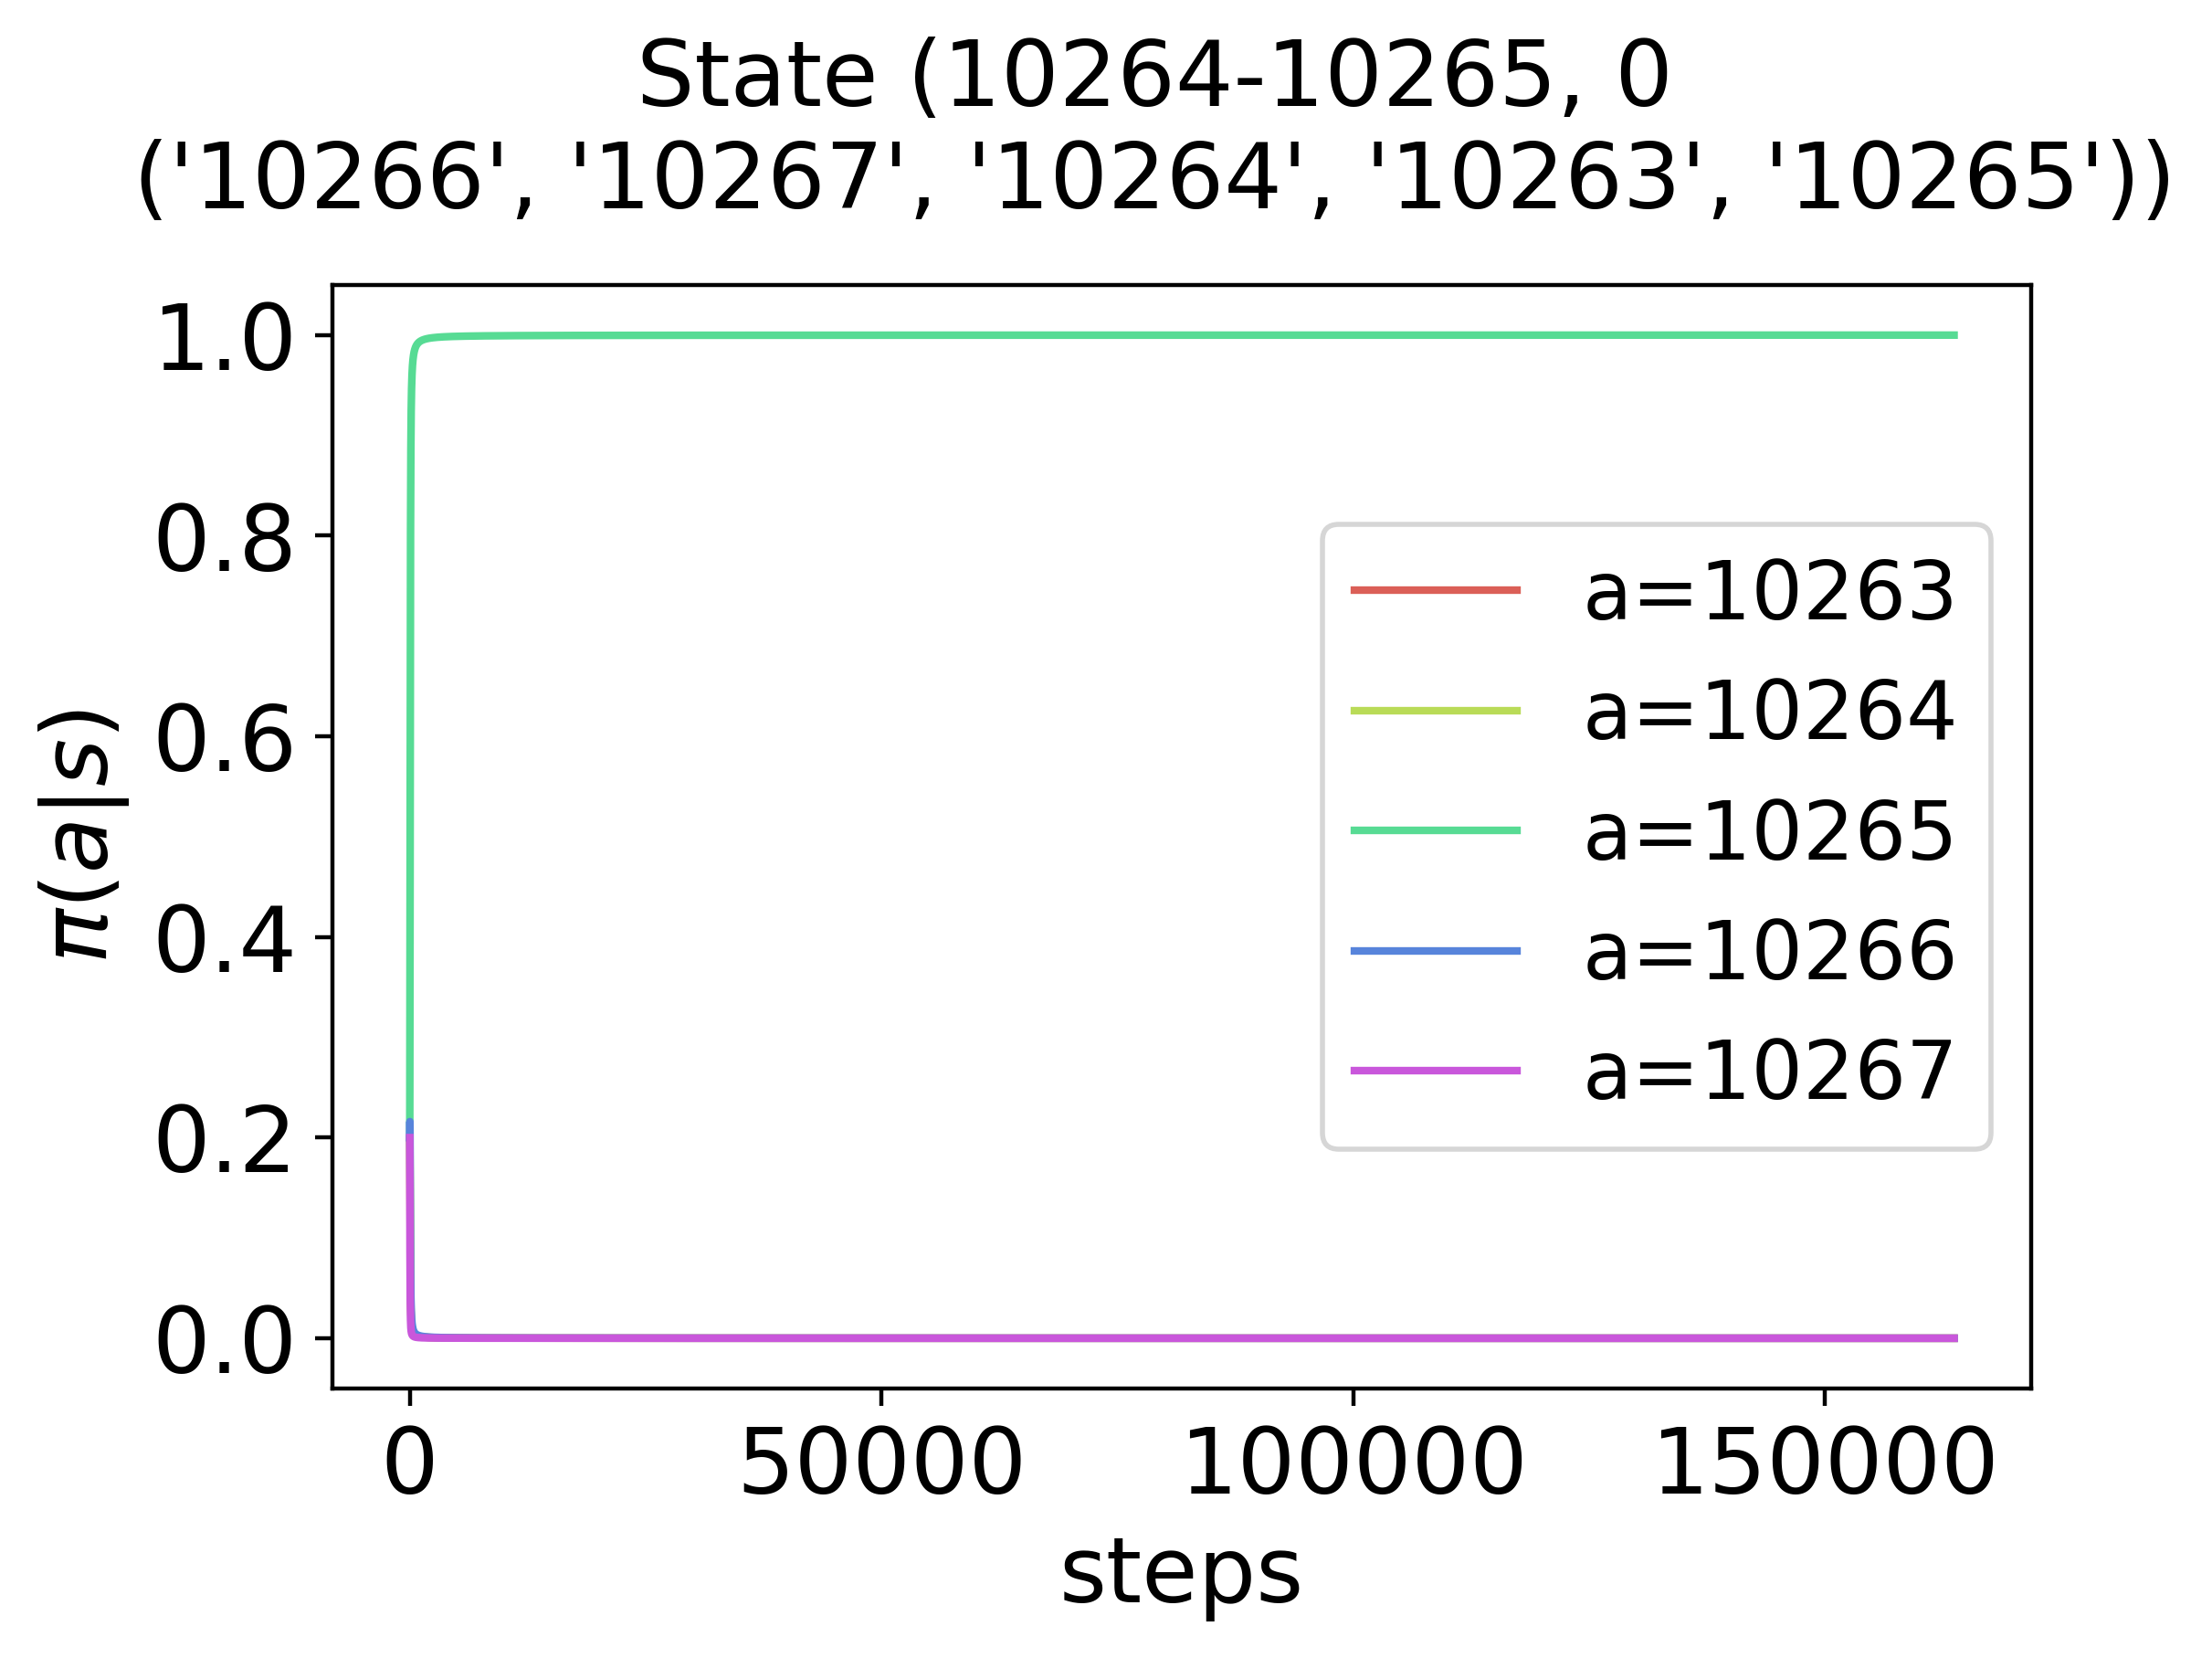
\includegraphics[scale=0.36,valign=b]{chapters/figures/policy_PG_state_0.png} &
        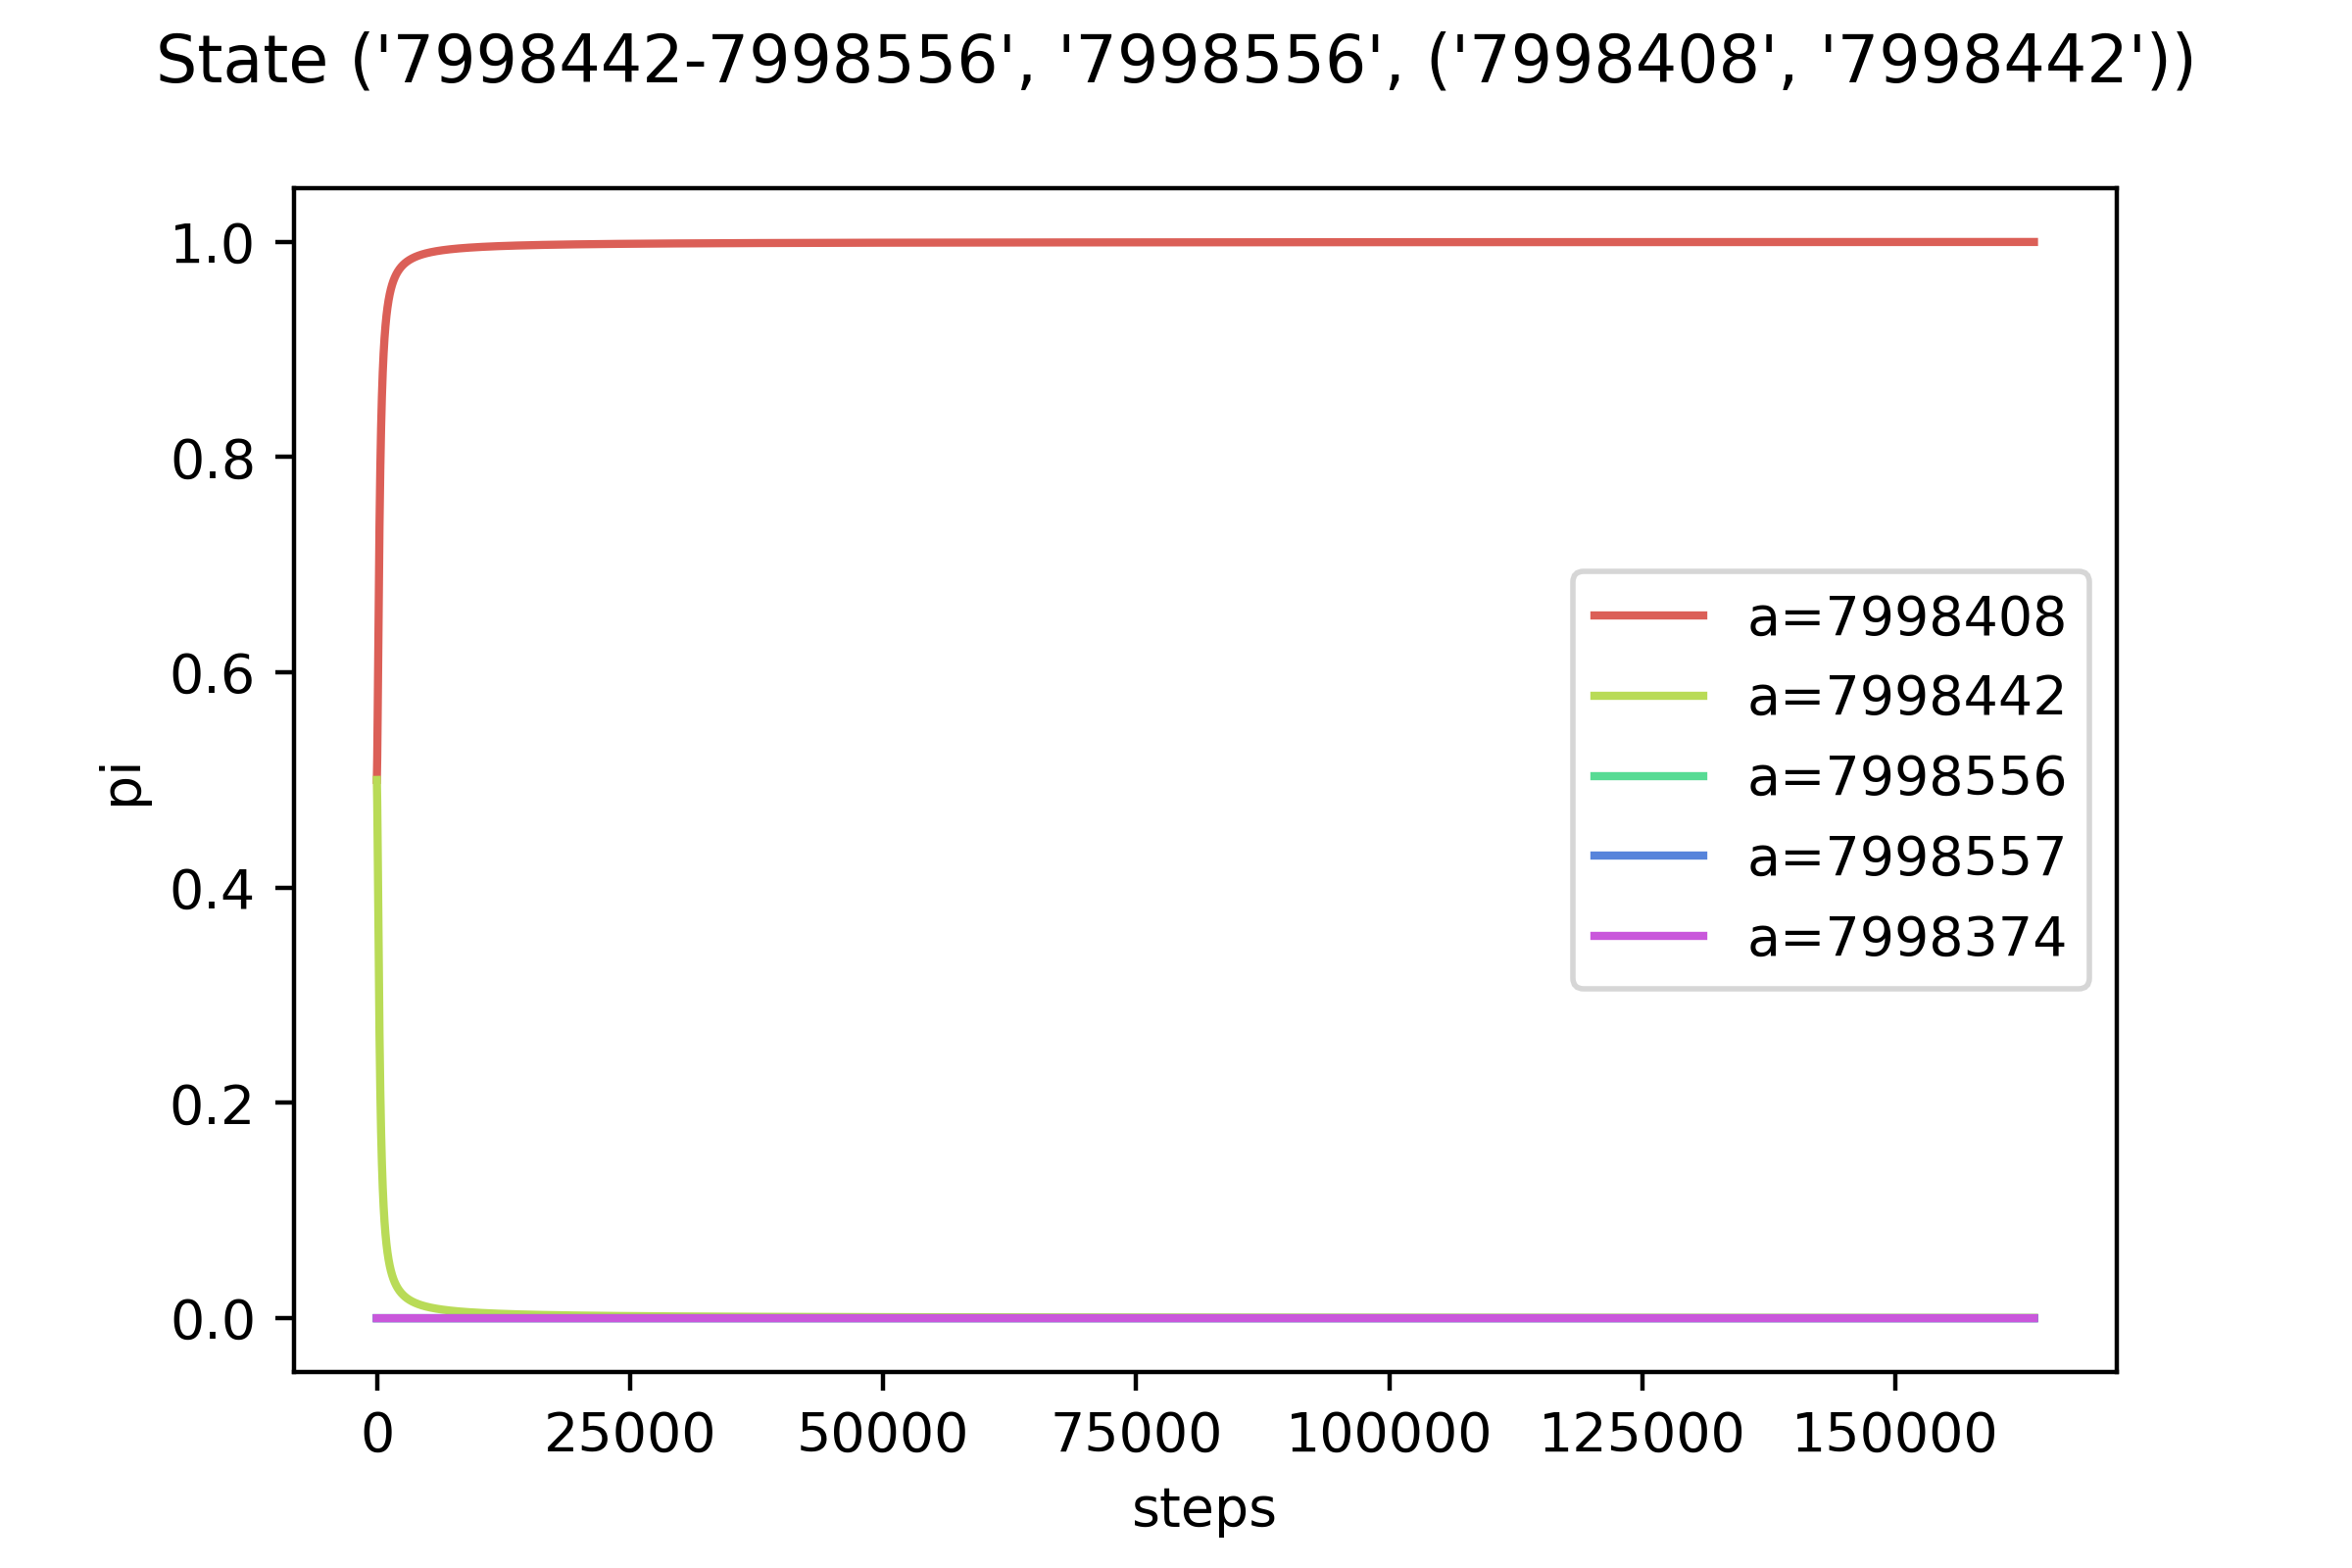
\includegraphics[scale=0.36,valign=b]{chapters/figures/policy_PG_state_1.png} \\
        \hspace*{-5pt}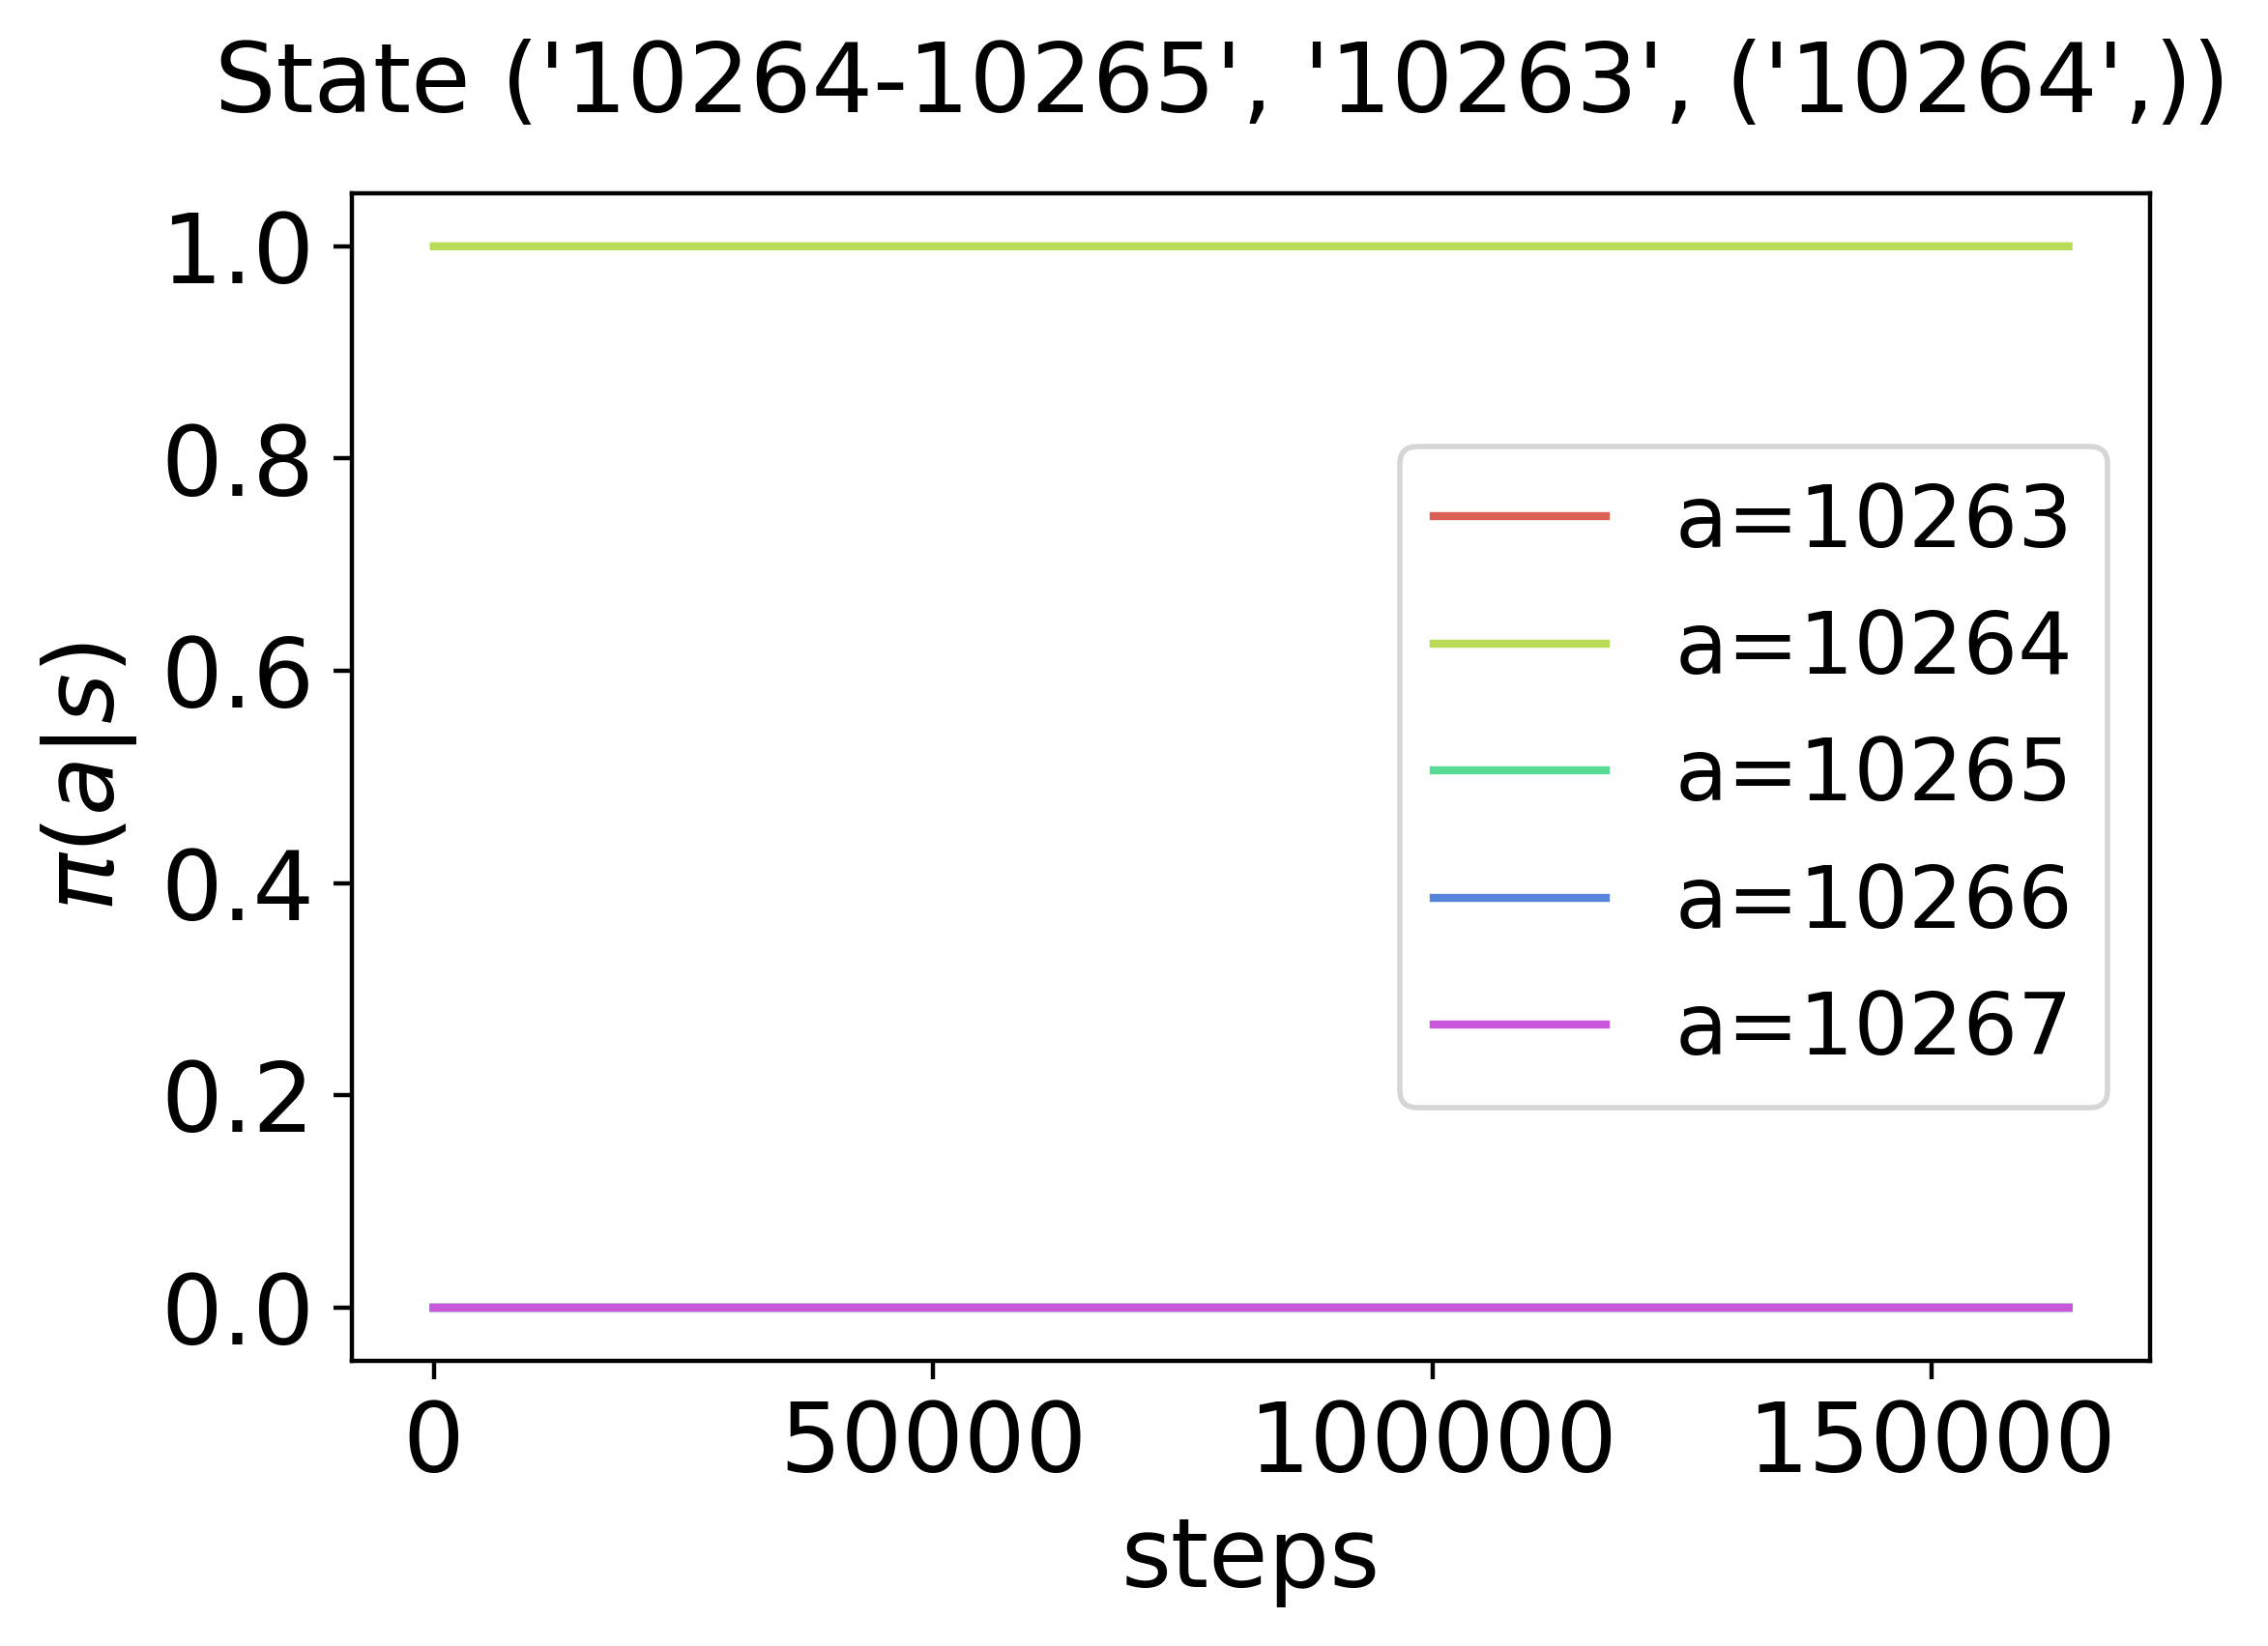
\includegraphics[scale=0.36,valign=b]{chapters/figures/policy_PG_state_2.png} &
        \hspace*{-18pt}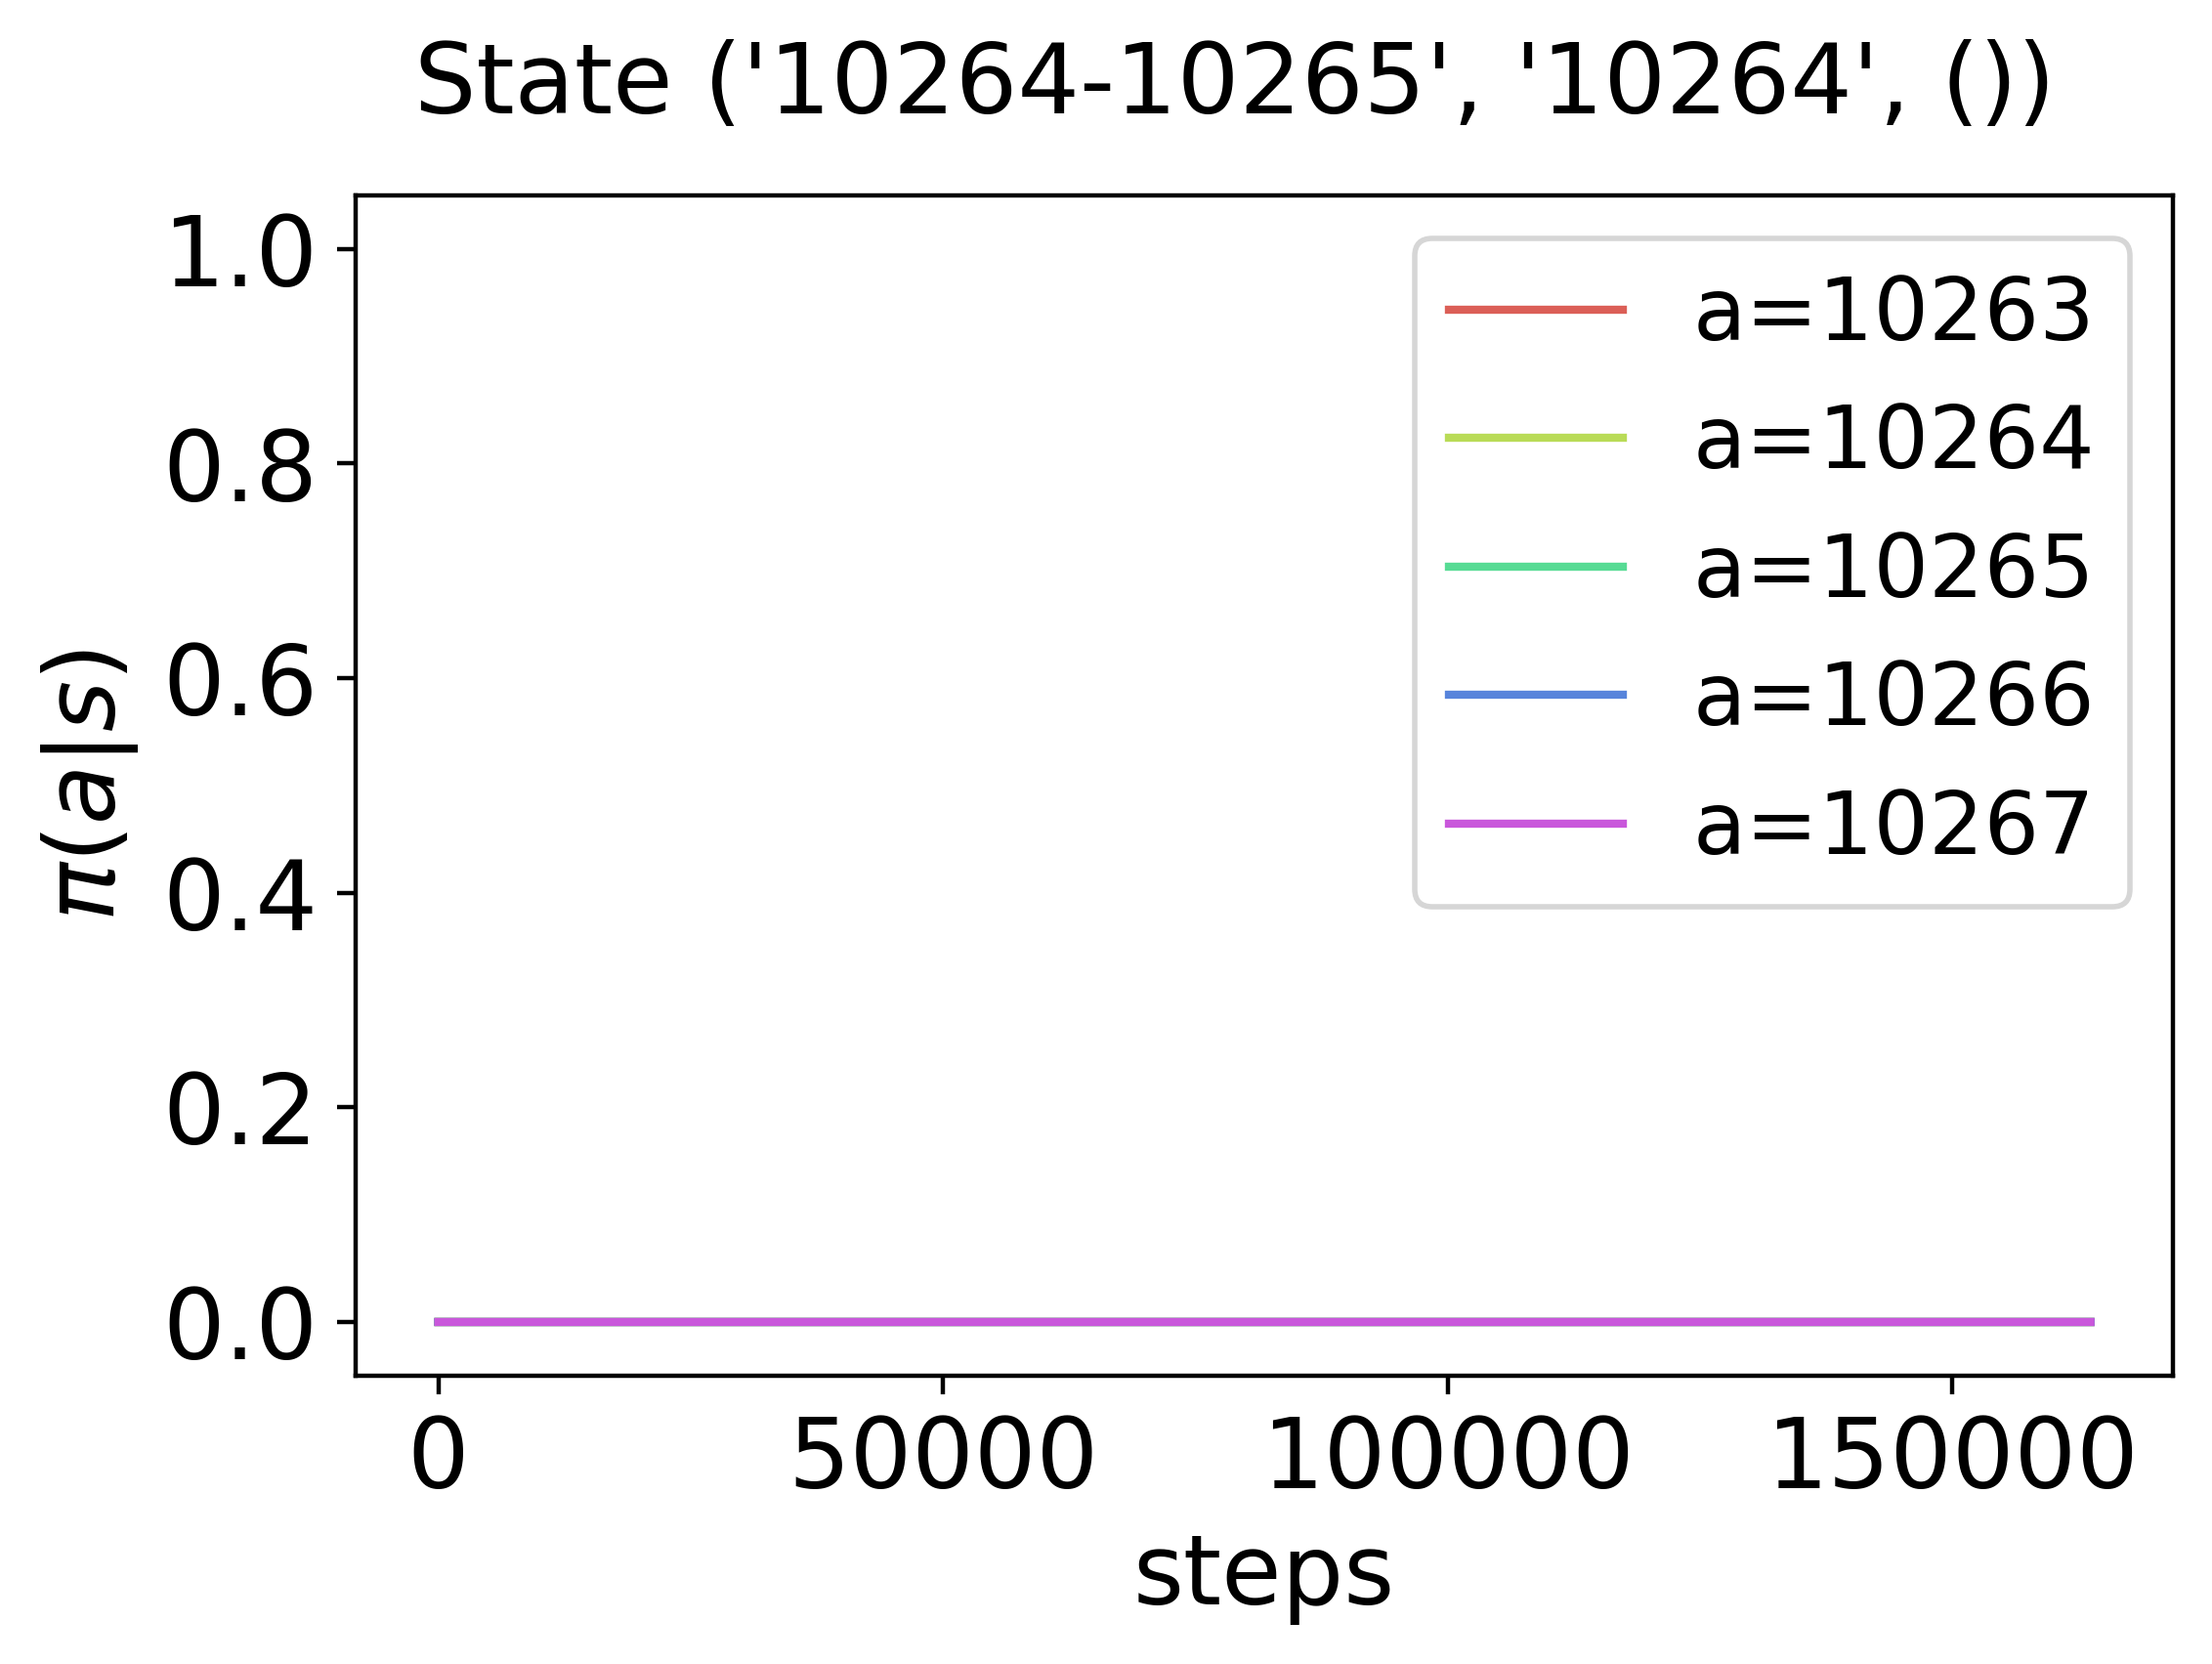
\includegraphics[scale=0.36,valign=b]{chapters/figures/policy_PG_state_3.png}
    \end{tabular}
    \caption{\small Trajectories of the policies $\pi_{\boldsymbol \theta}$ in the policy space for \acrshort{pg}, in the exact same previous setting.}
    \label{fig:sequence-policies-pg}
\end{figure}

\begin{figure}[!htp]
    \centering
    \begin{tabular}{cc}
        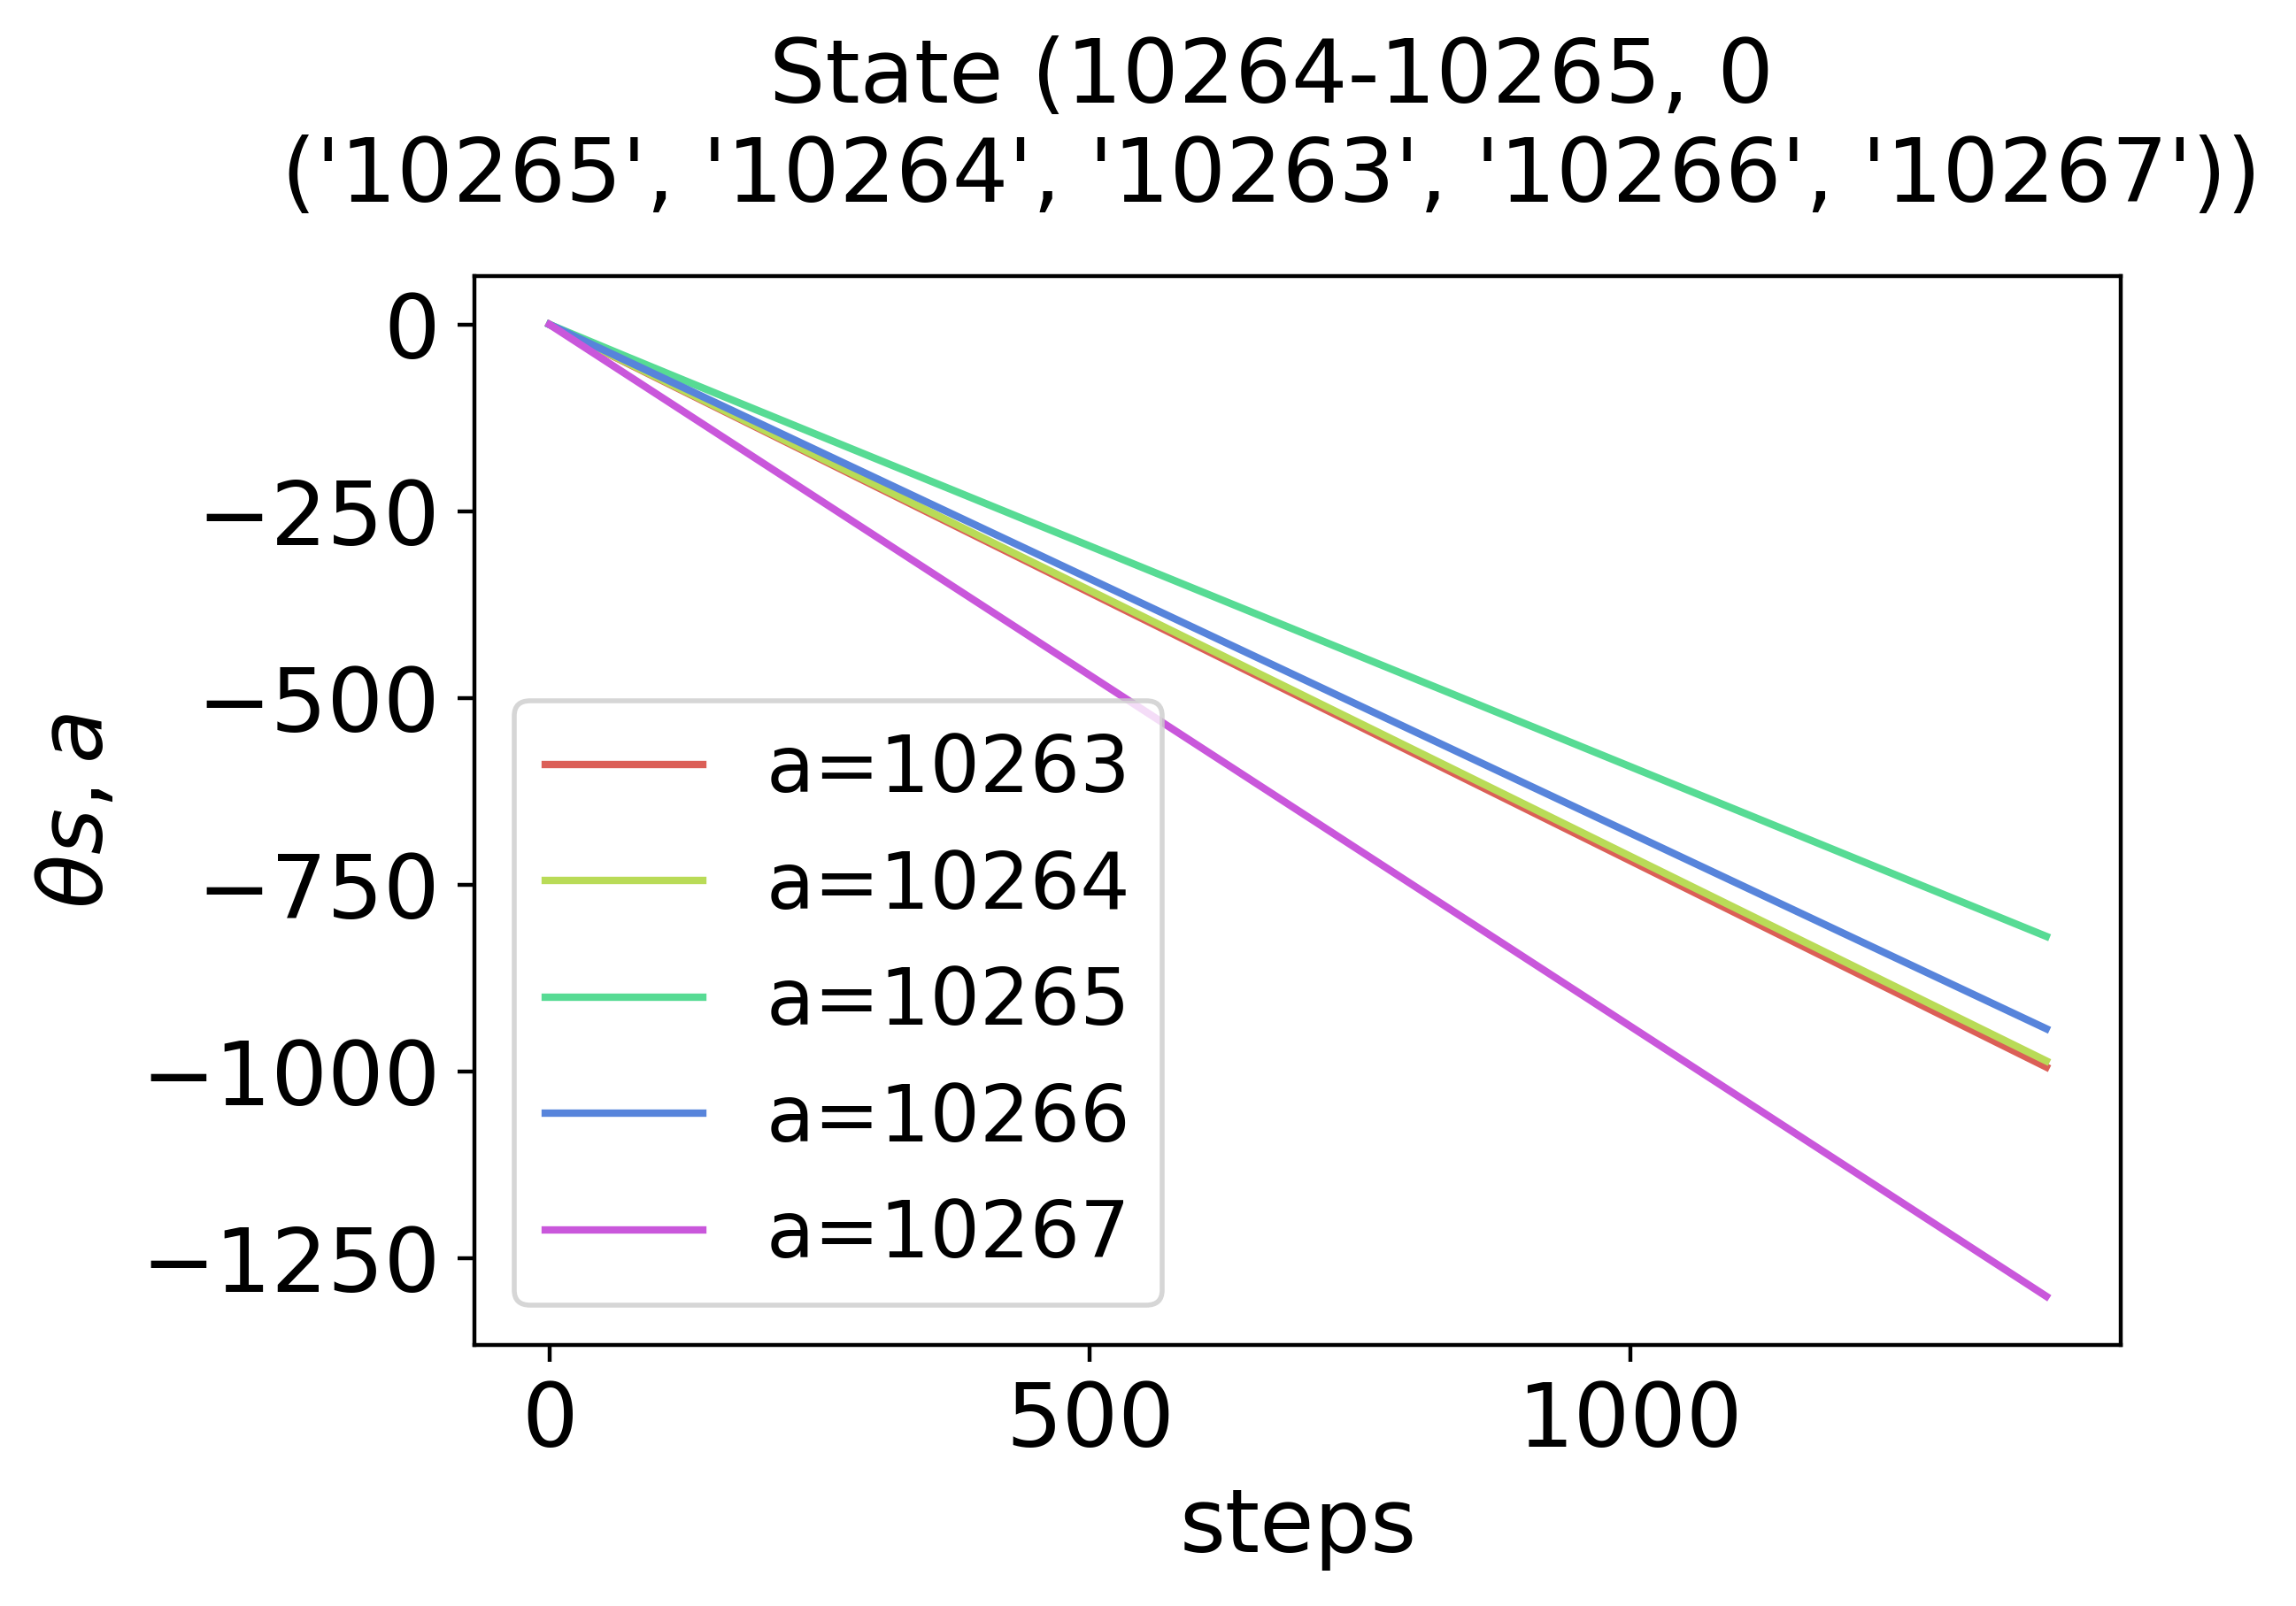
\includegraphics[scale=0.36,valign=b]{chapters/figures/theta_NPG_state_0.png} &
        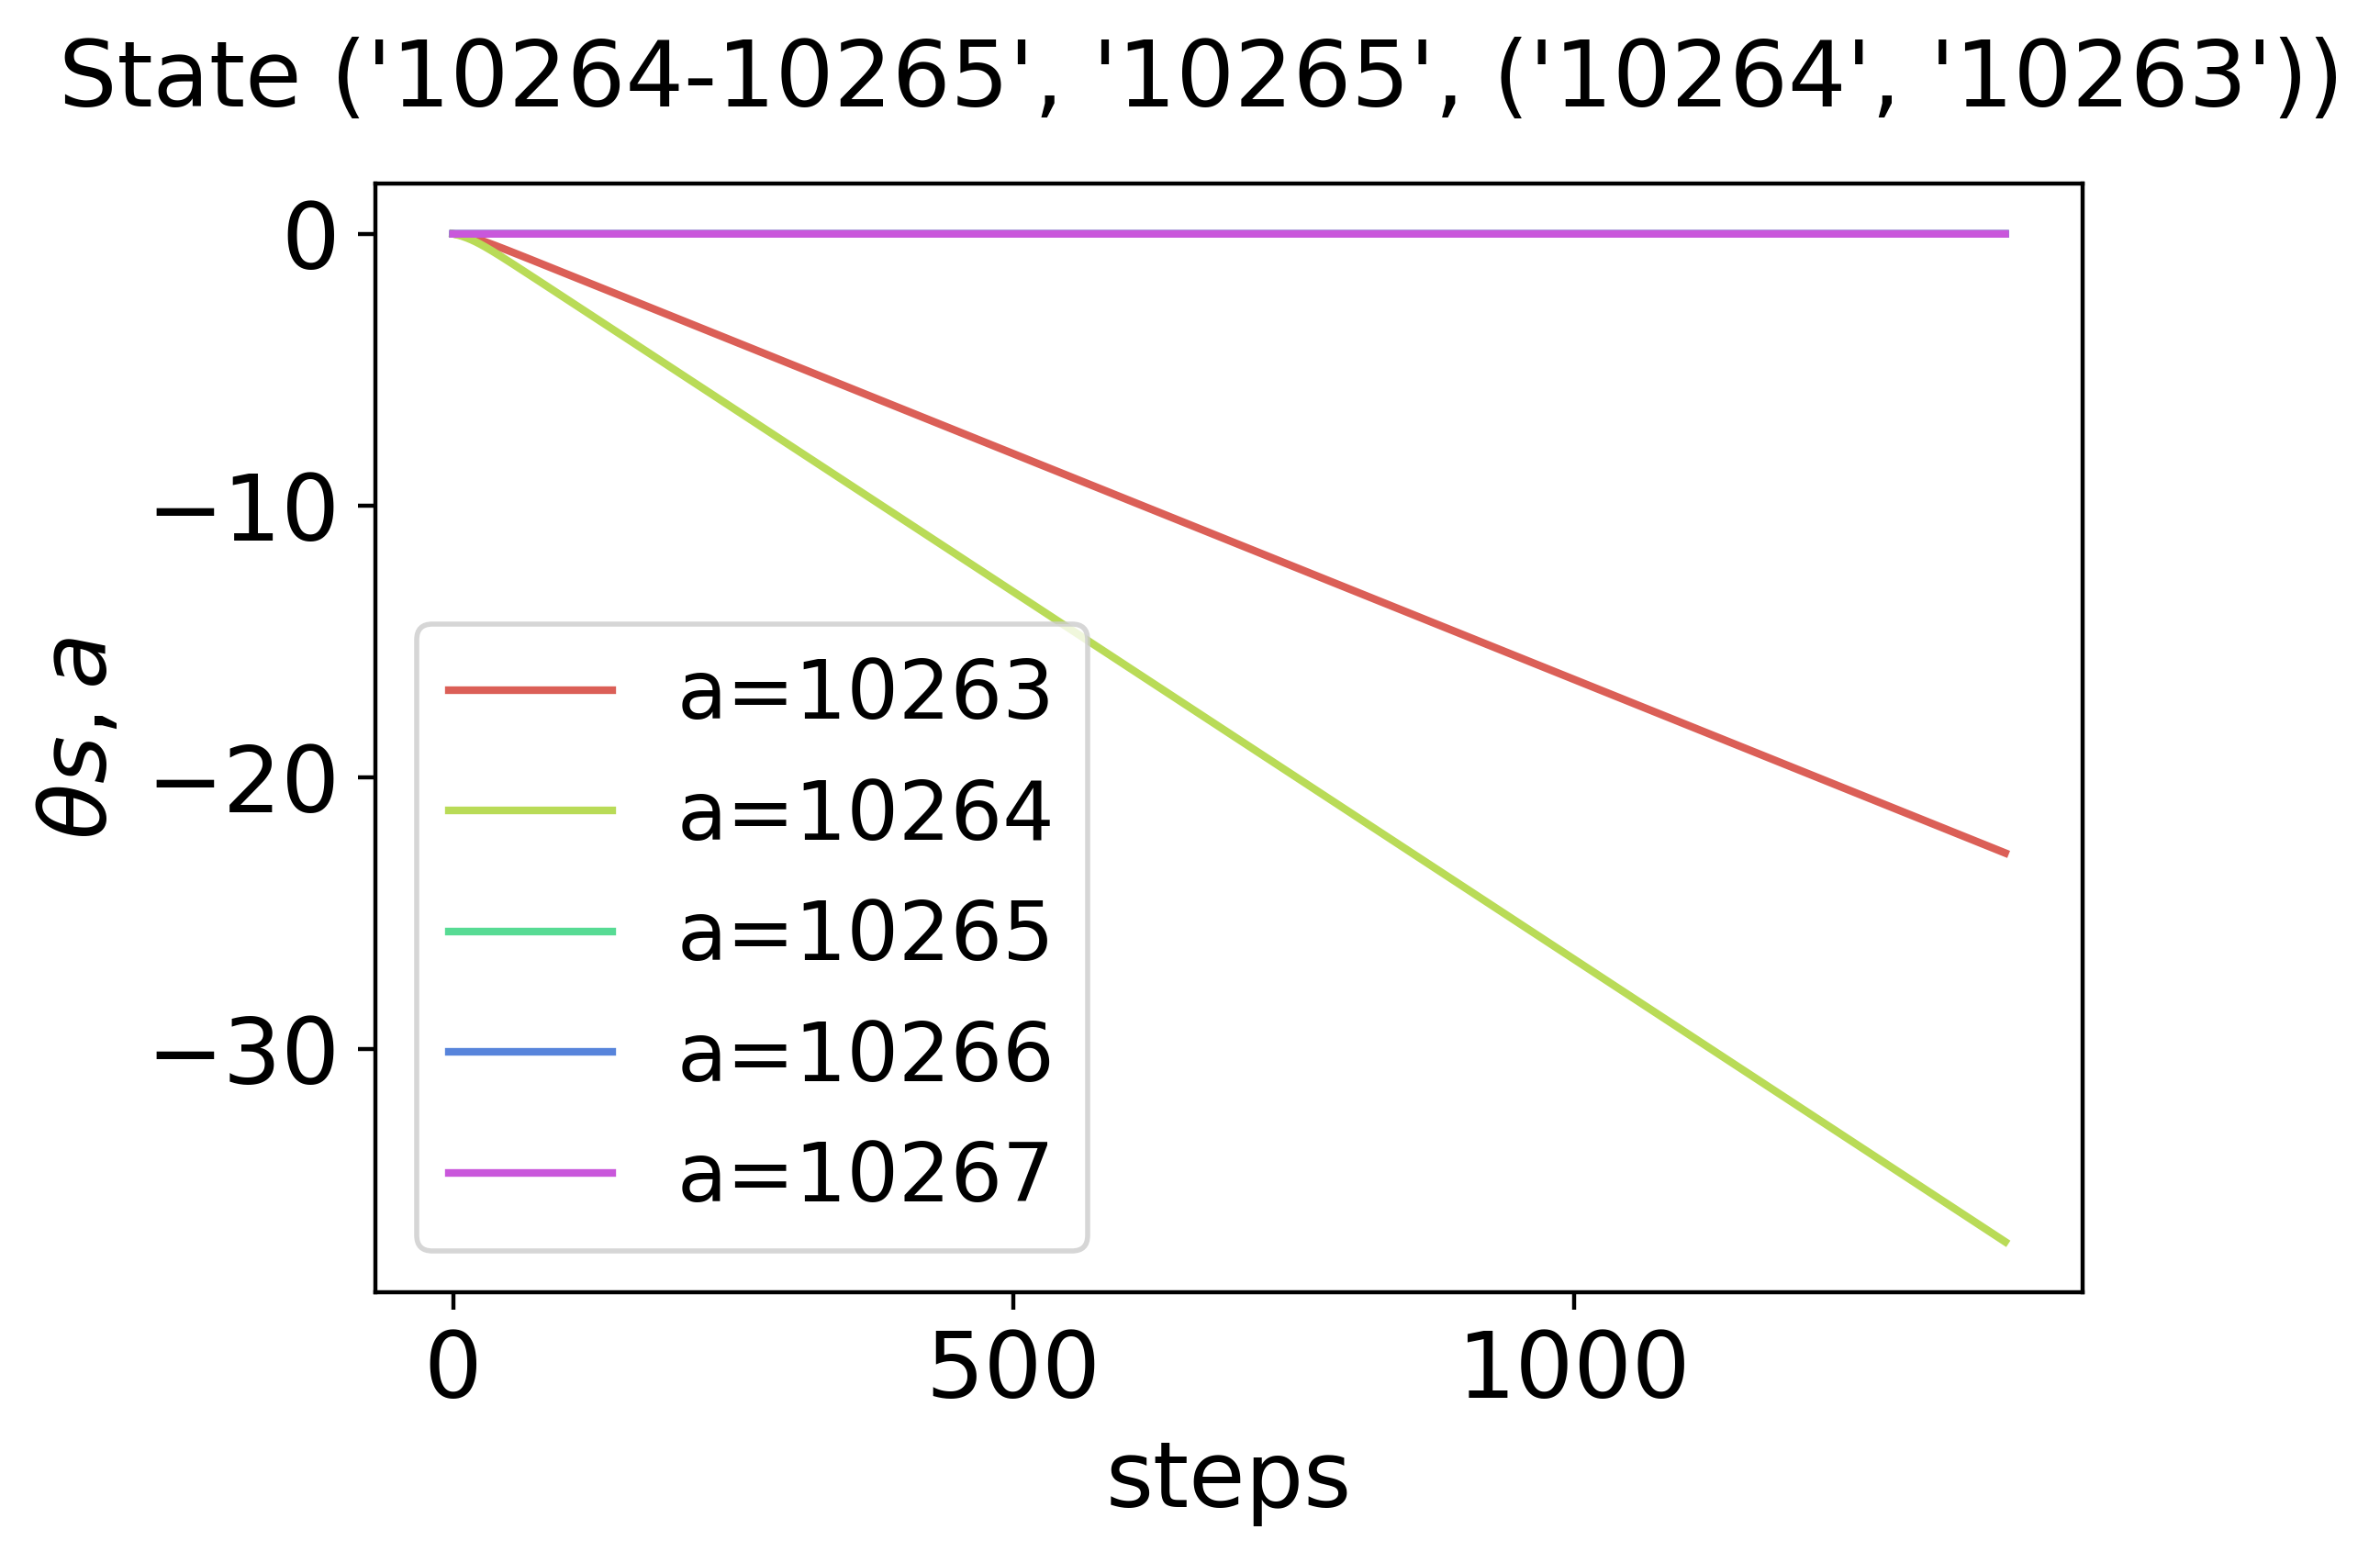
\includegraphics[scale=0.36,valign=b]{chapters/figures/theta_NPG_state_1.png} \\
        \hspace*{9pt}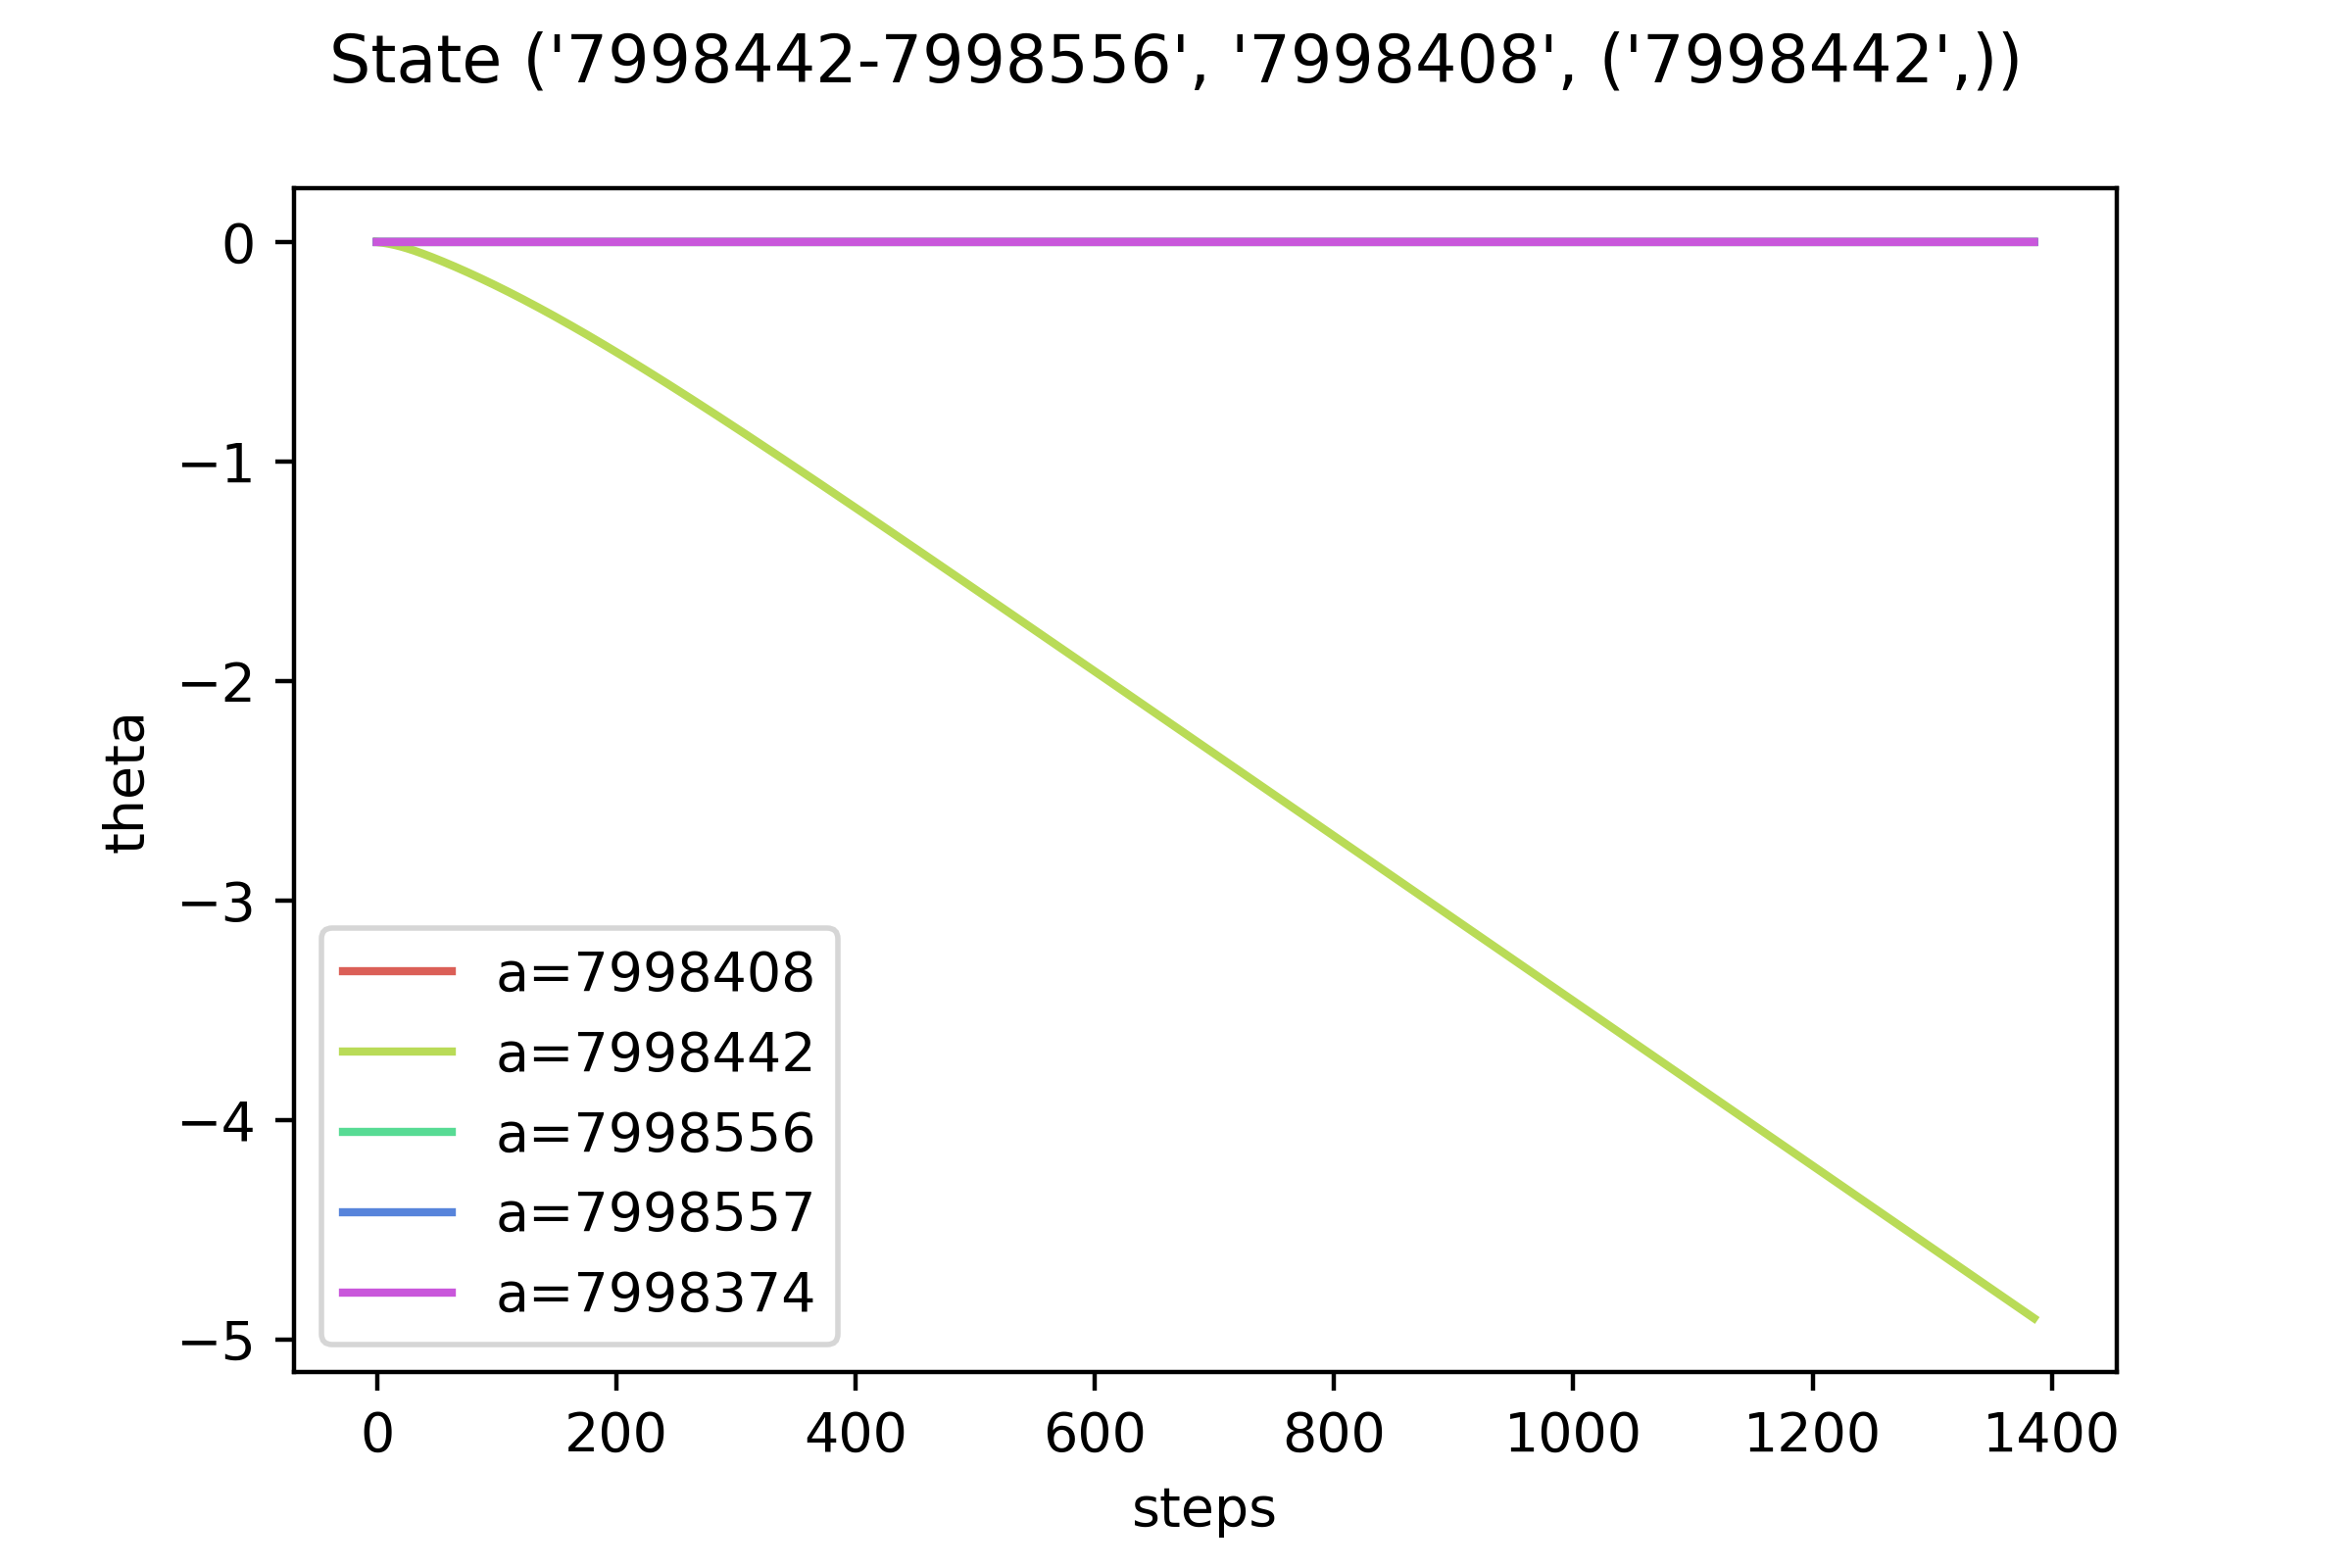
\includegraphics[scale=0.36,valign=b]{chapters/figures/theta_NPG_state_2.png} &
        \hspace*{-26.7pt}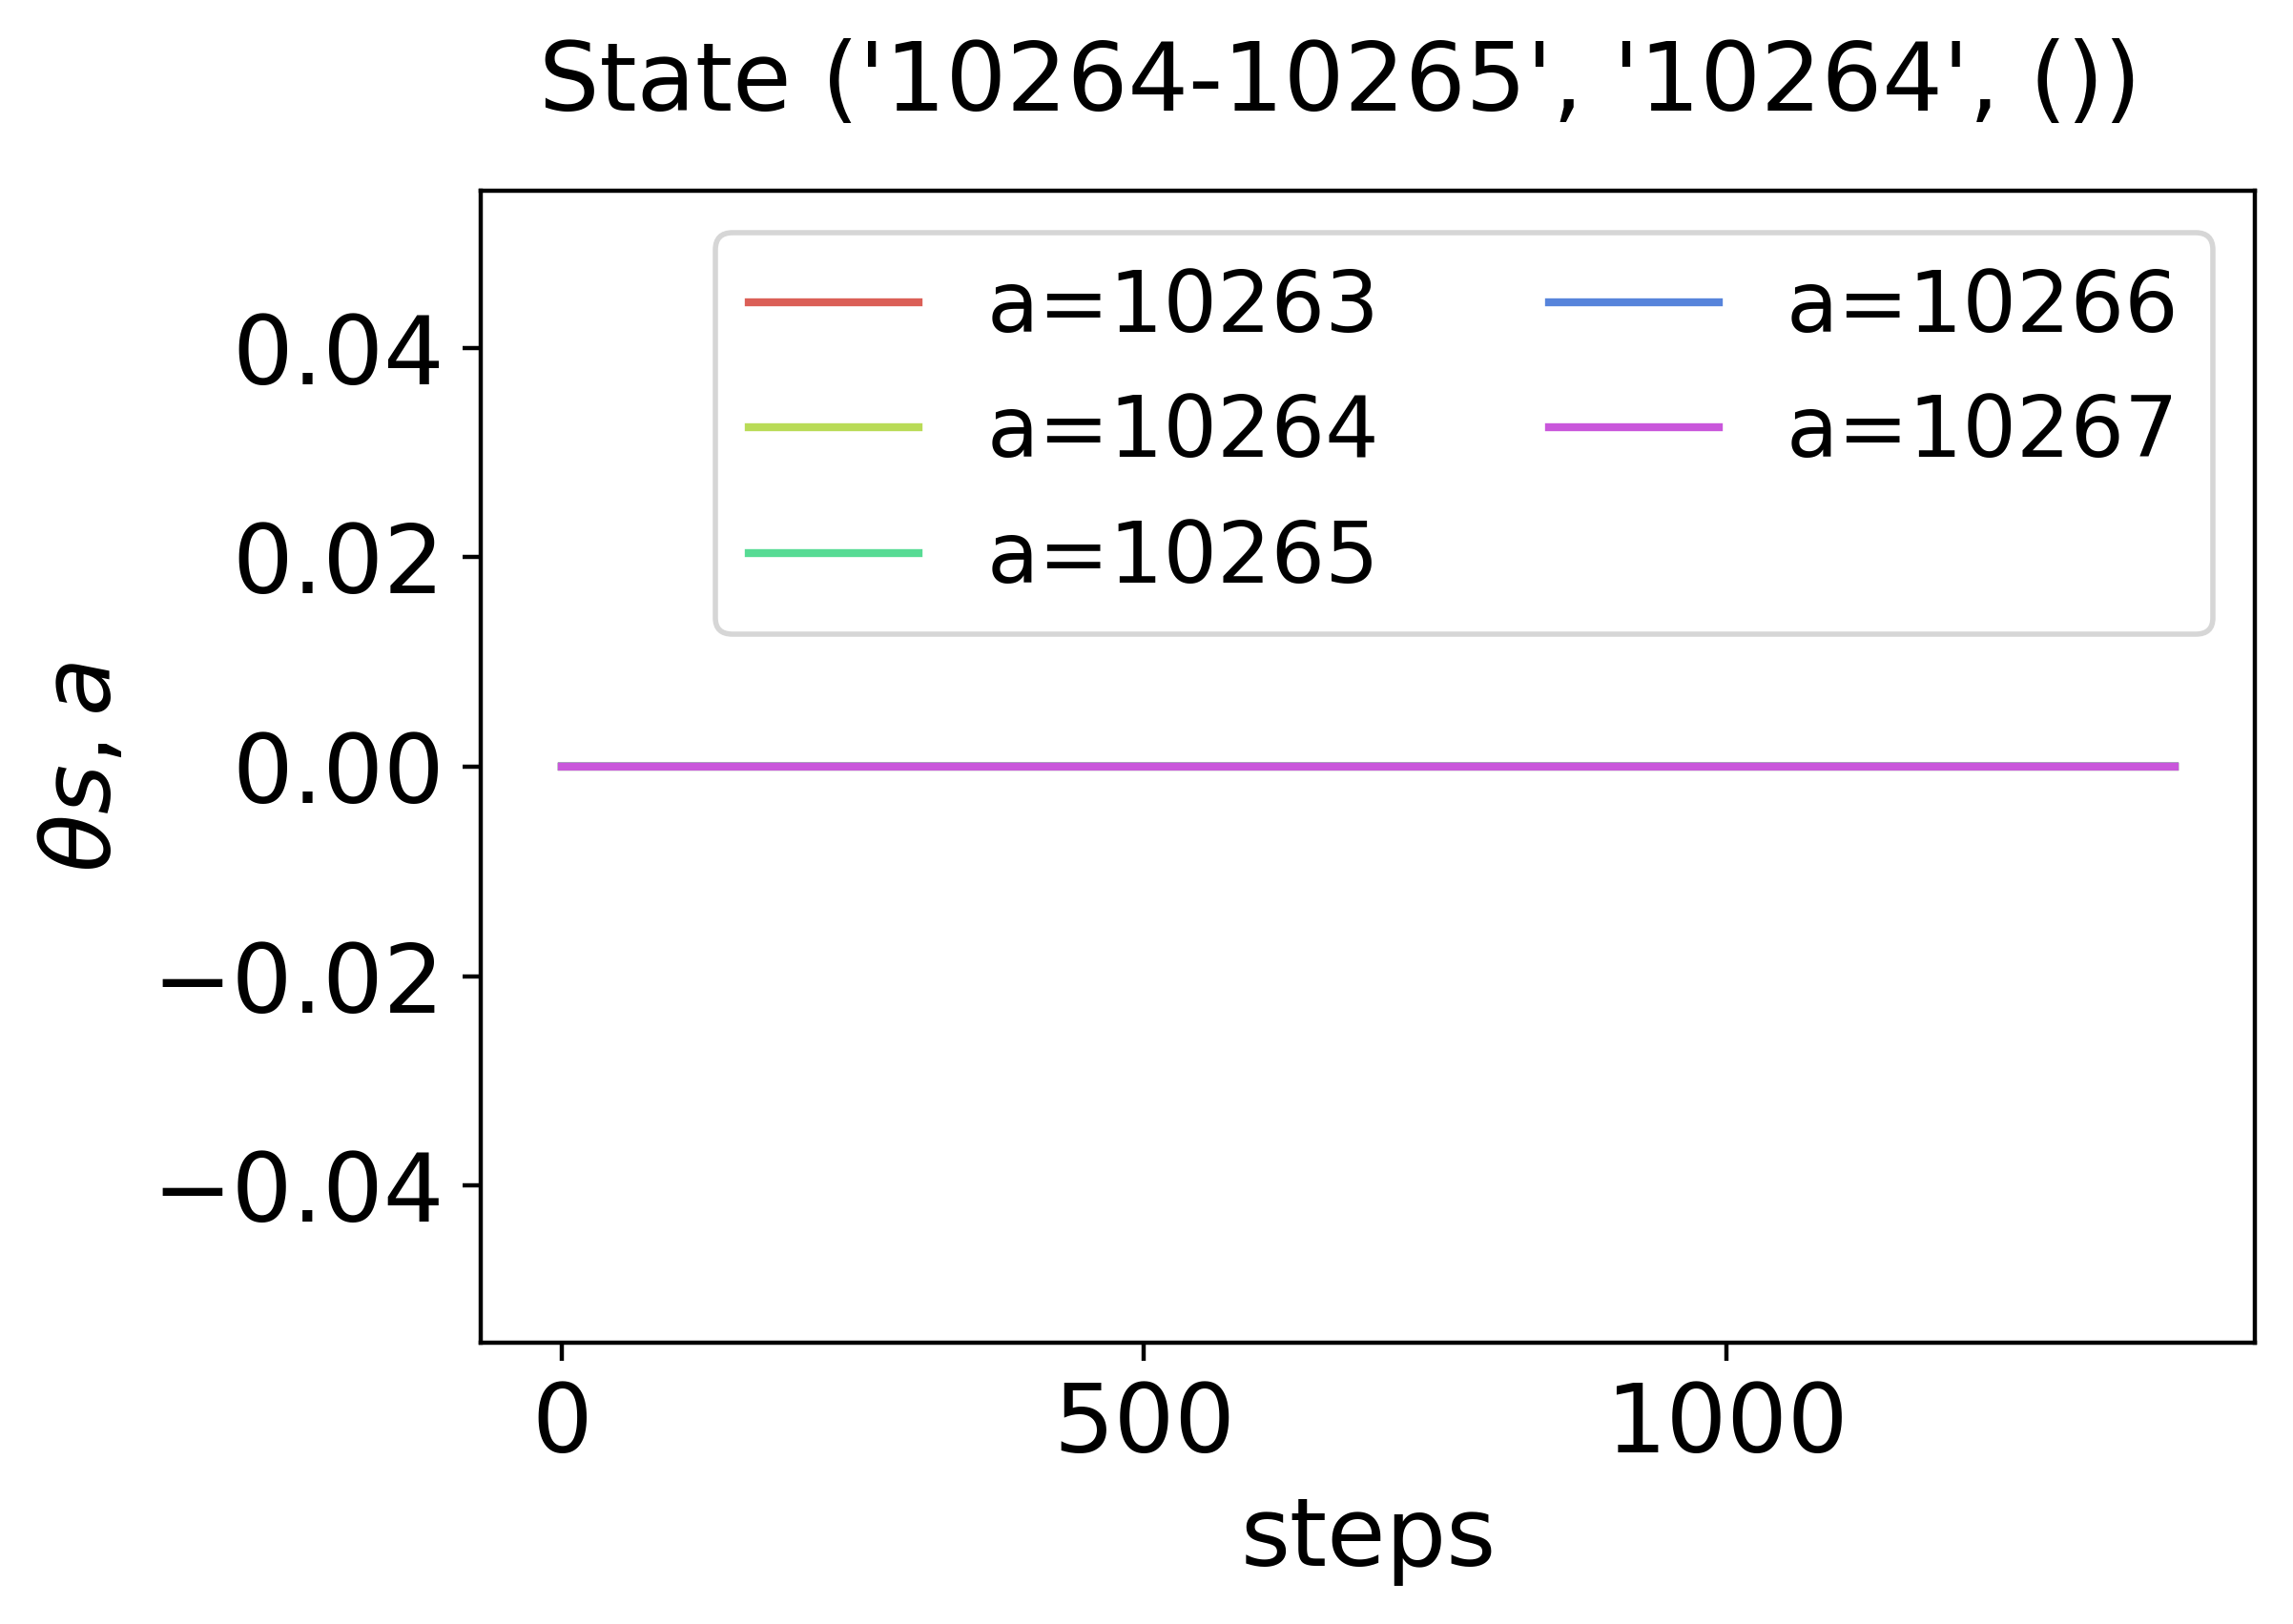
\includegraphics[scale=0.36,valign=b]{chapters/figures/theta_NPG_state_3.png}
    \end{tabular}
    \caption{Trajectories of the parameters $\boldsymbol \theta$ in the parameters space for \acrshort{npg}, for a specific episode (which starts in the top-left corner and goes from left to right, line by line) with $5$ initially disconnected substation.}
    \label{fig:sequence-theta-npg}
\end{figure}

\begin{figure}[!htp]
    \centering
    \begin{tabular}{cc}
        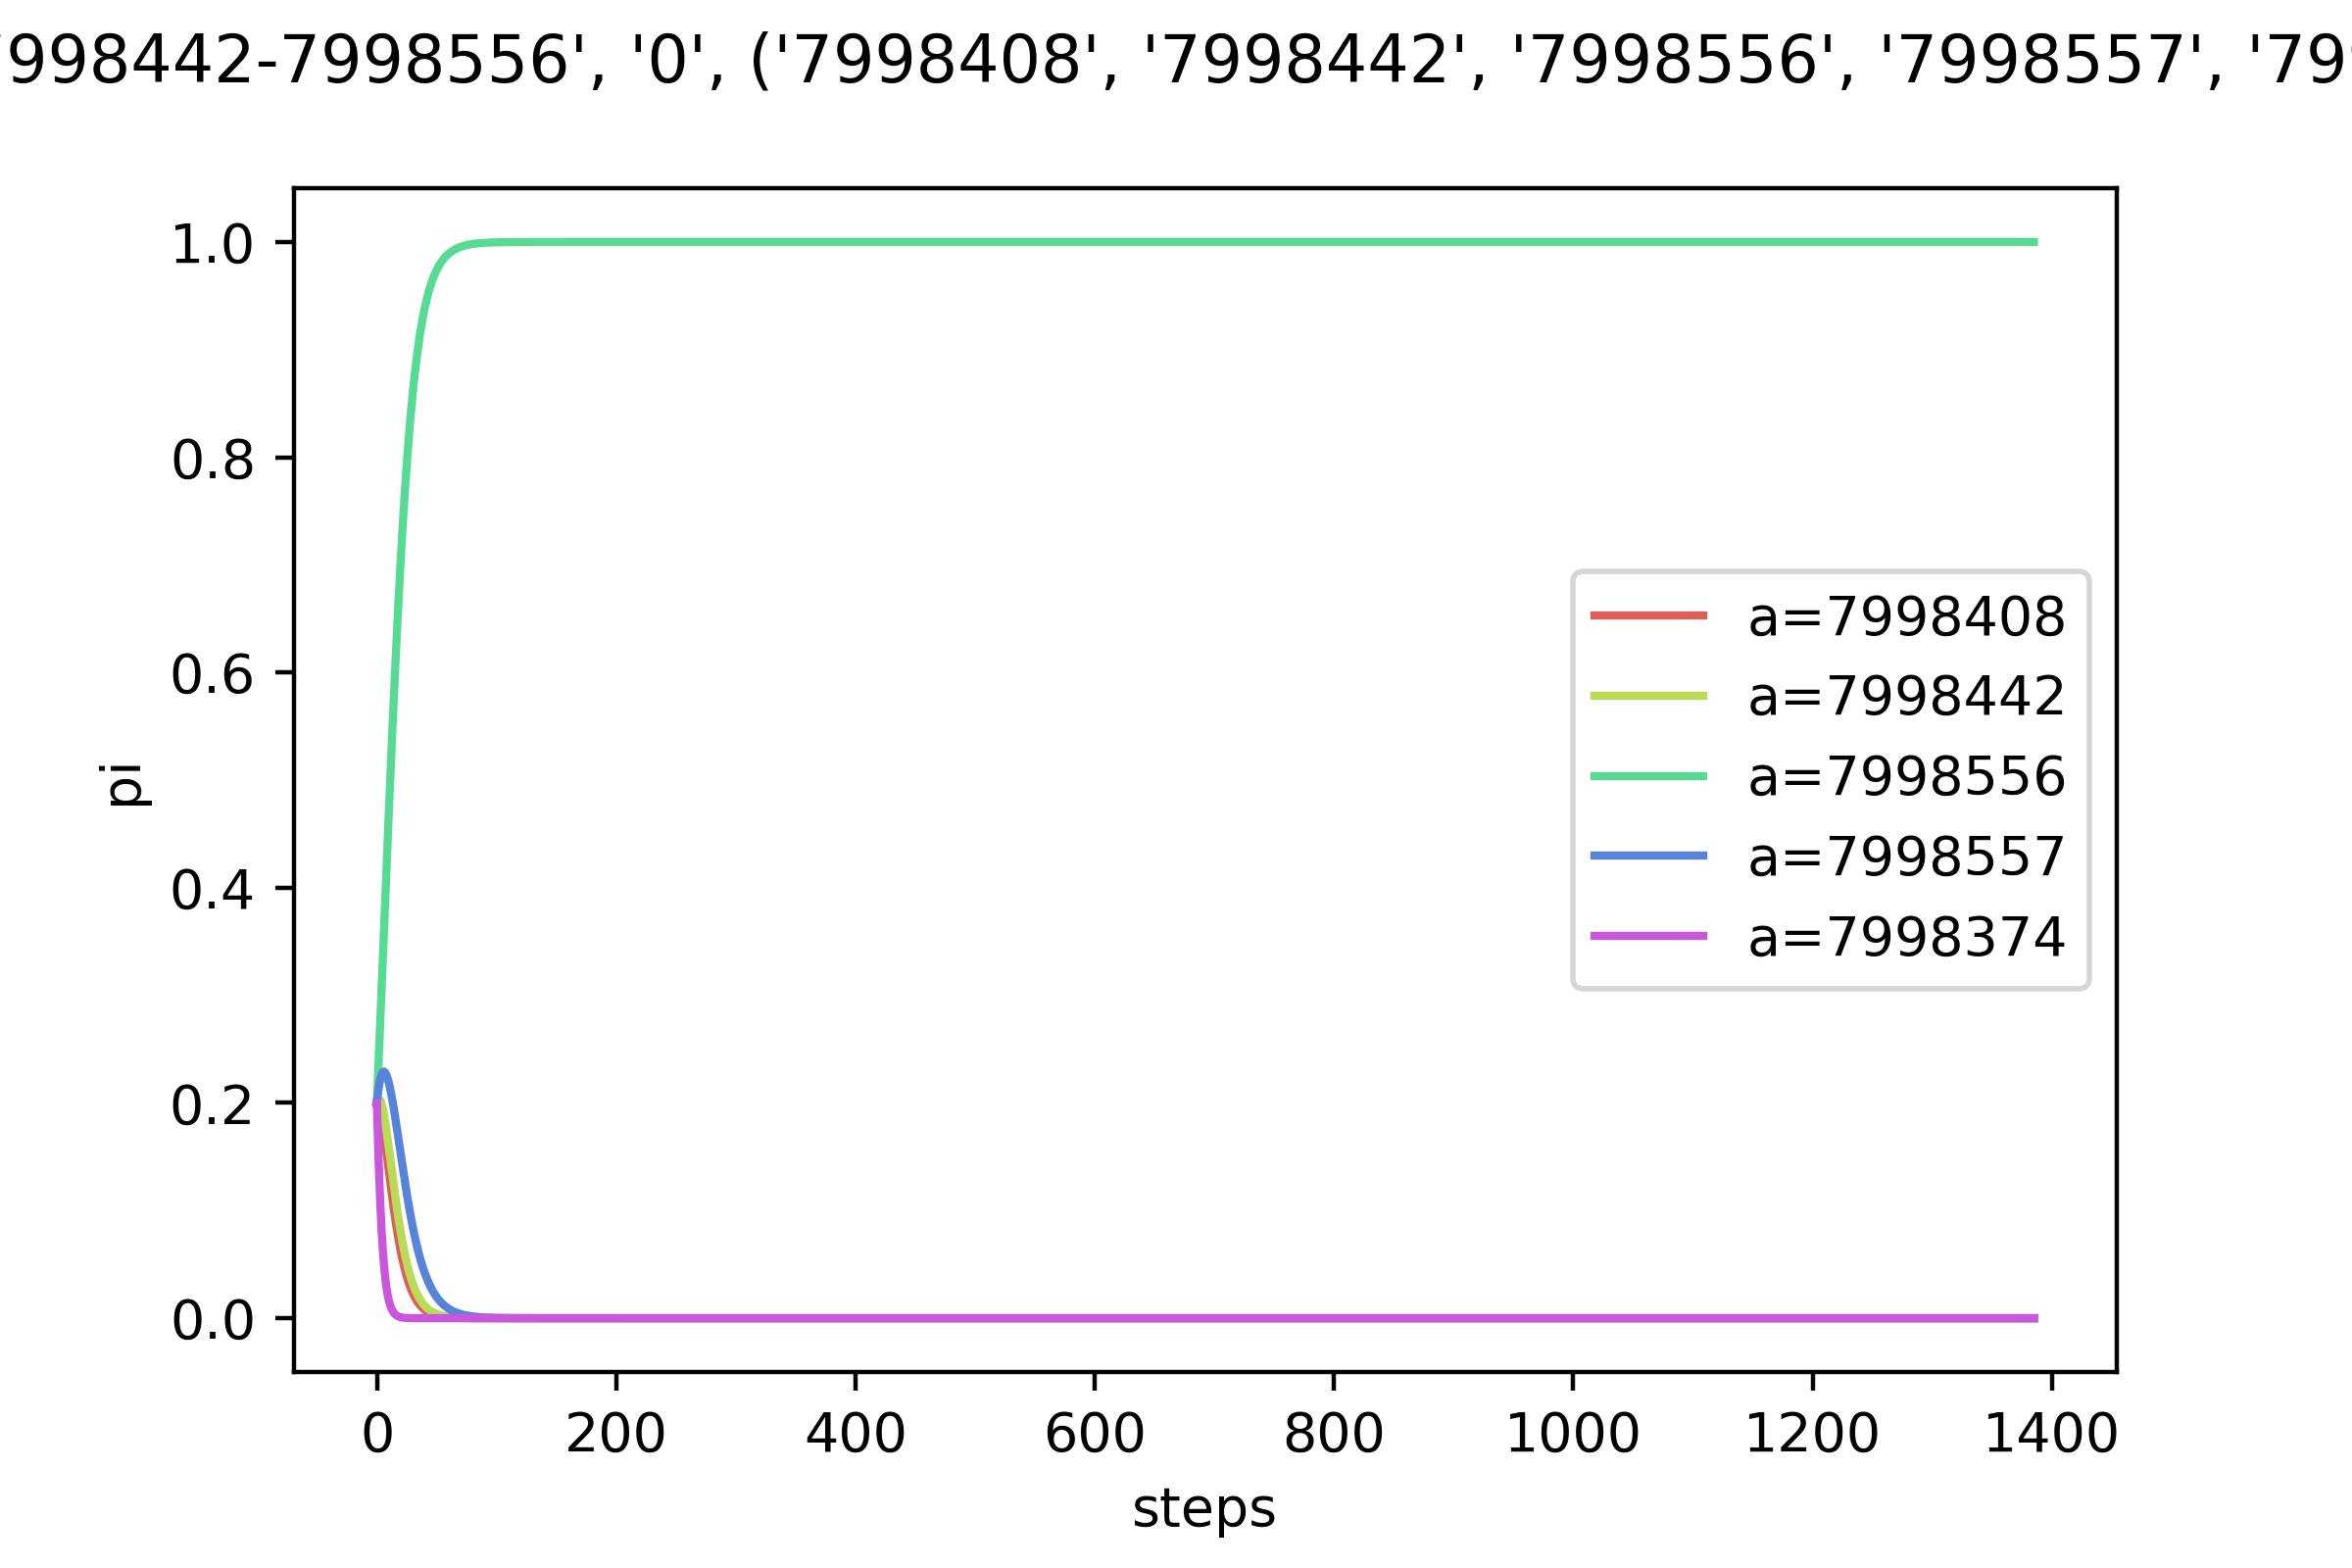
\includegraphics[scale=0.36,valign=b]{chapters/figures/policy_NPG_state_0.png} &
        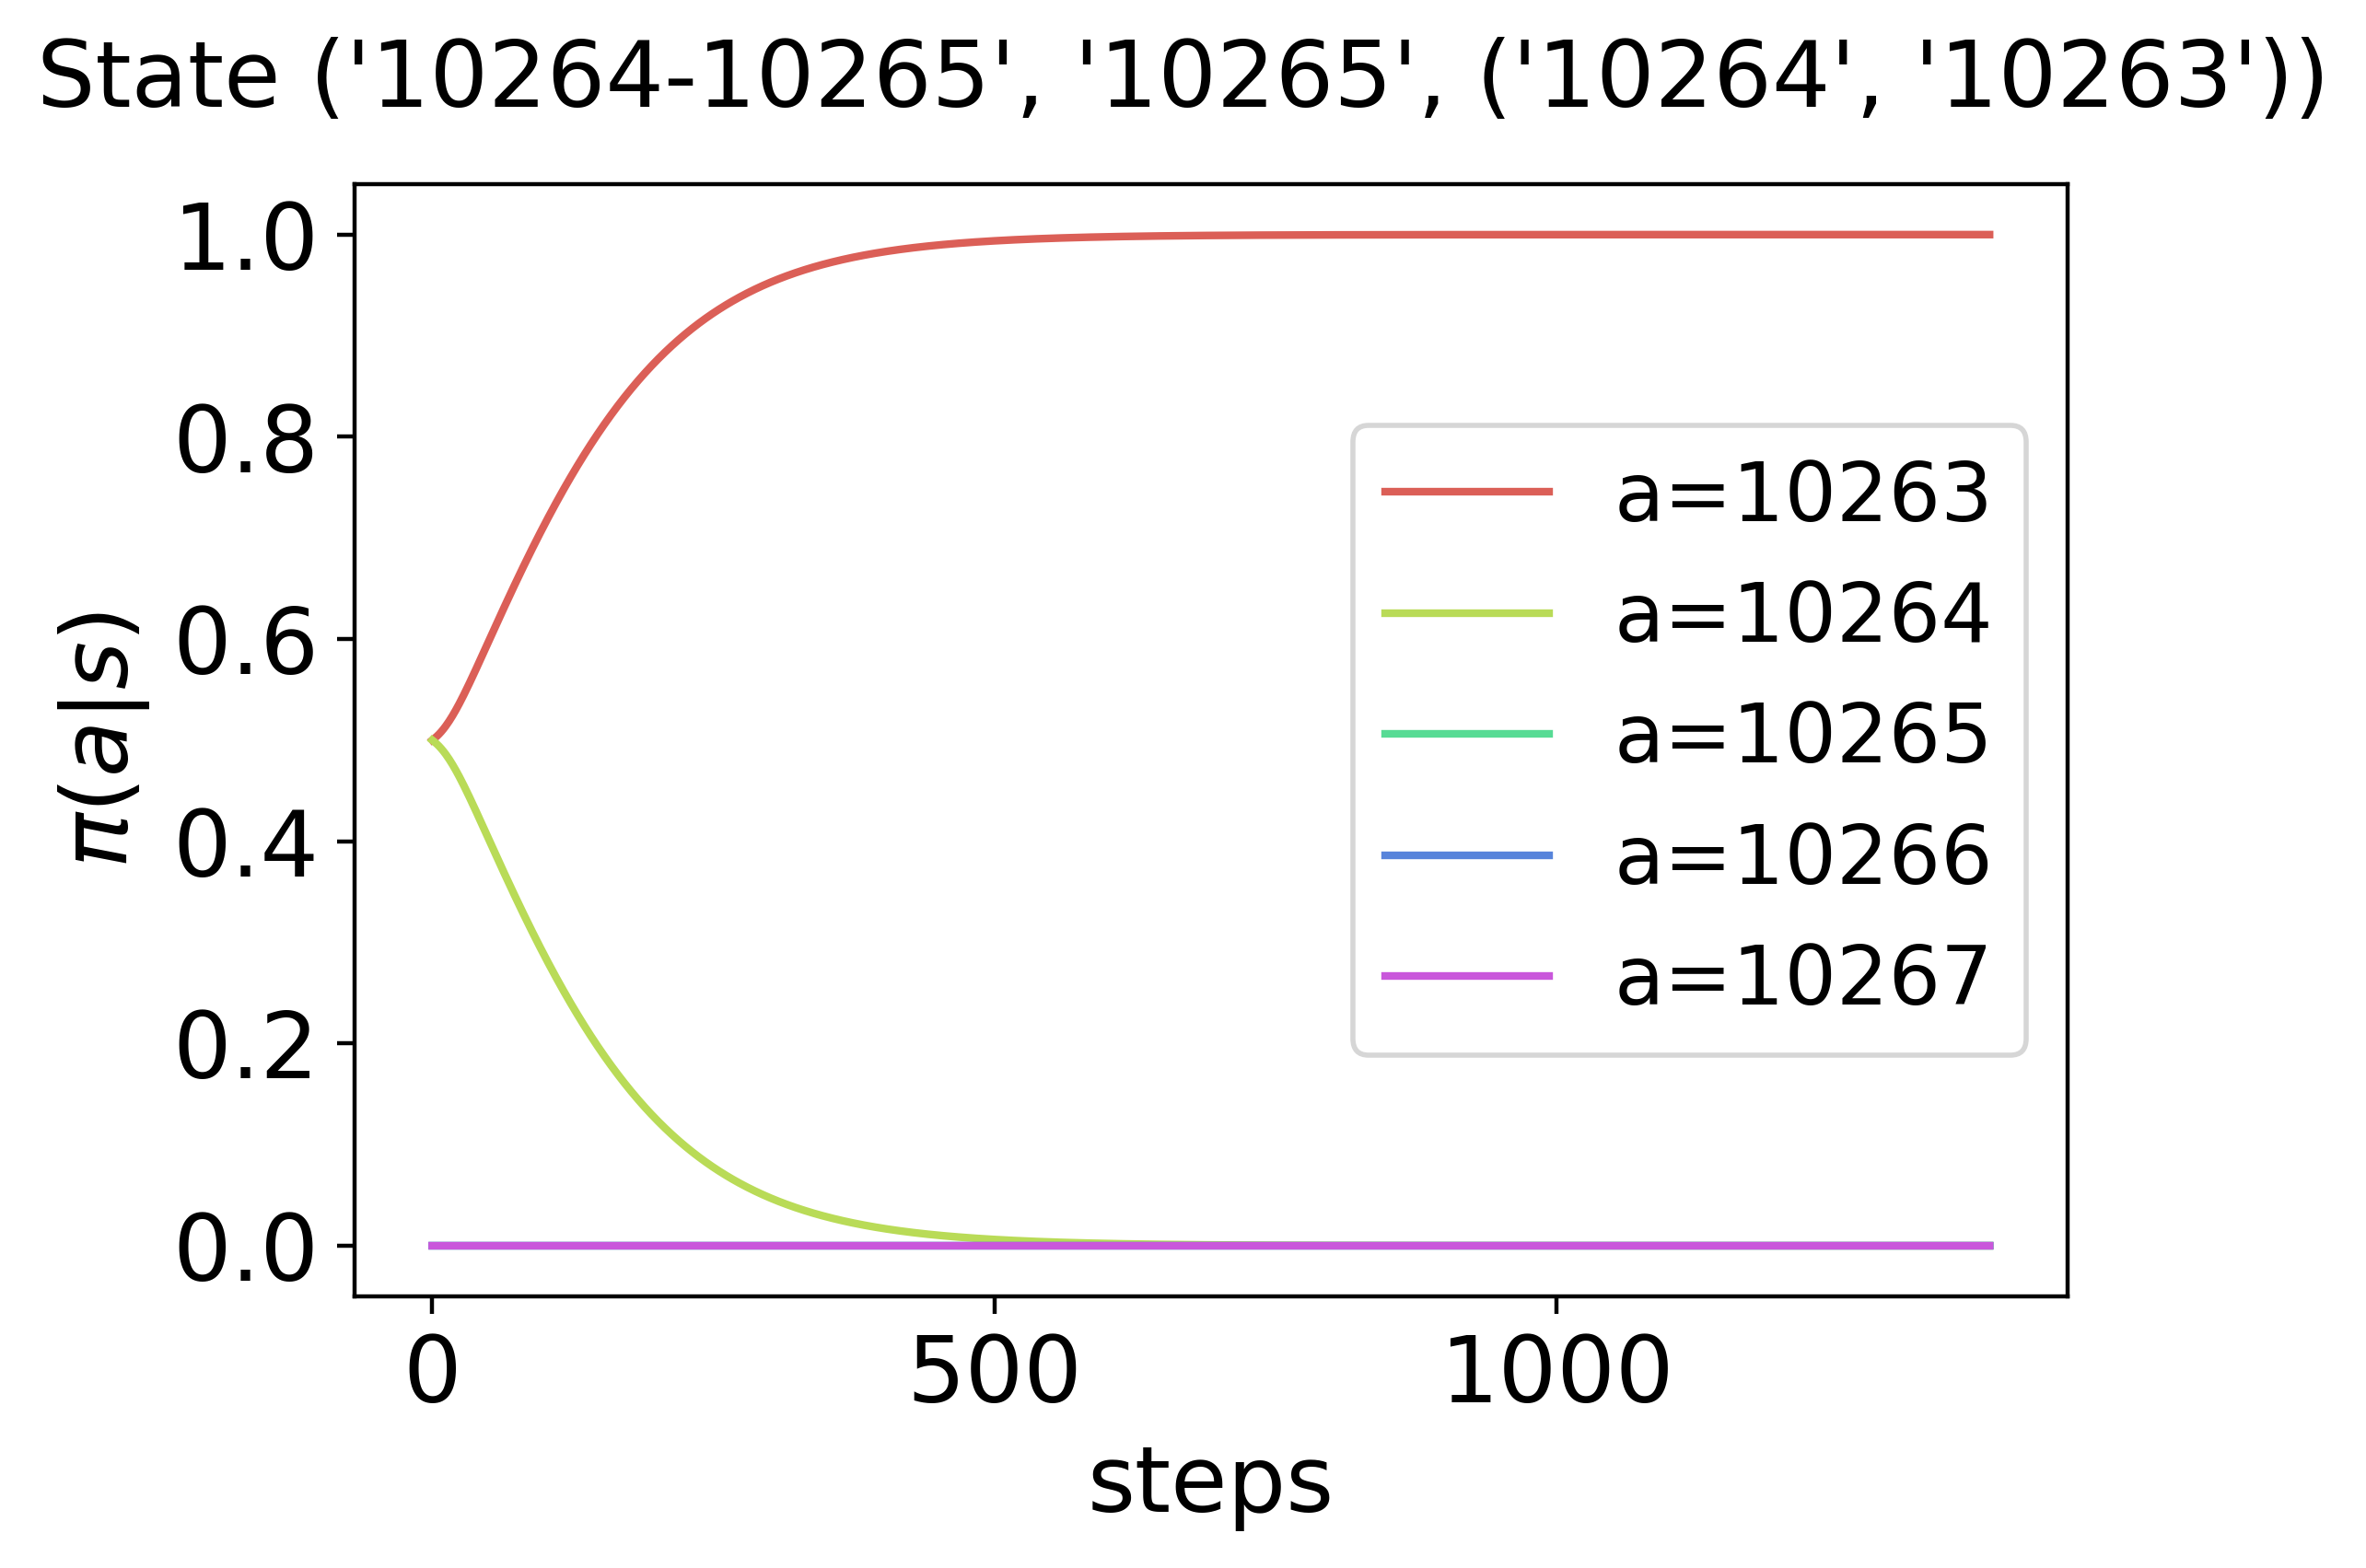
\includegraphics[scale=0.36,valign=b]{chapters/figures/policy_NPG_state_1.png} \\
        \hspace*{-5pt}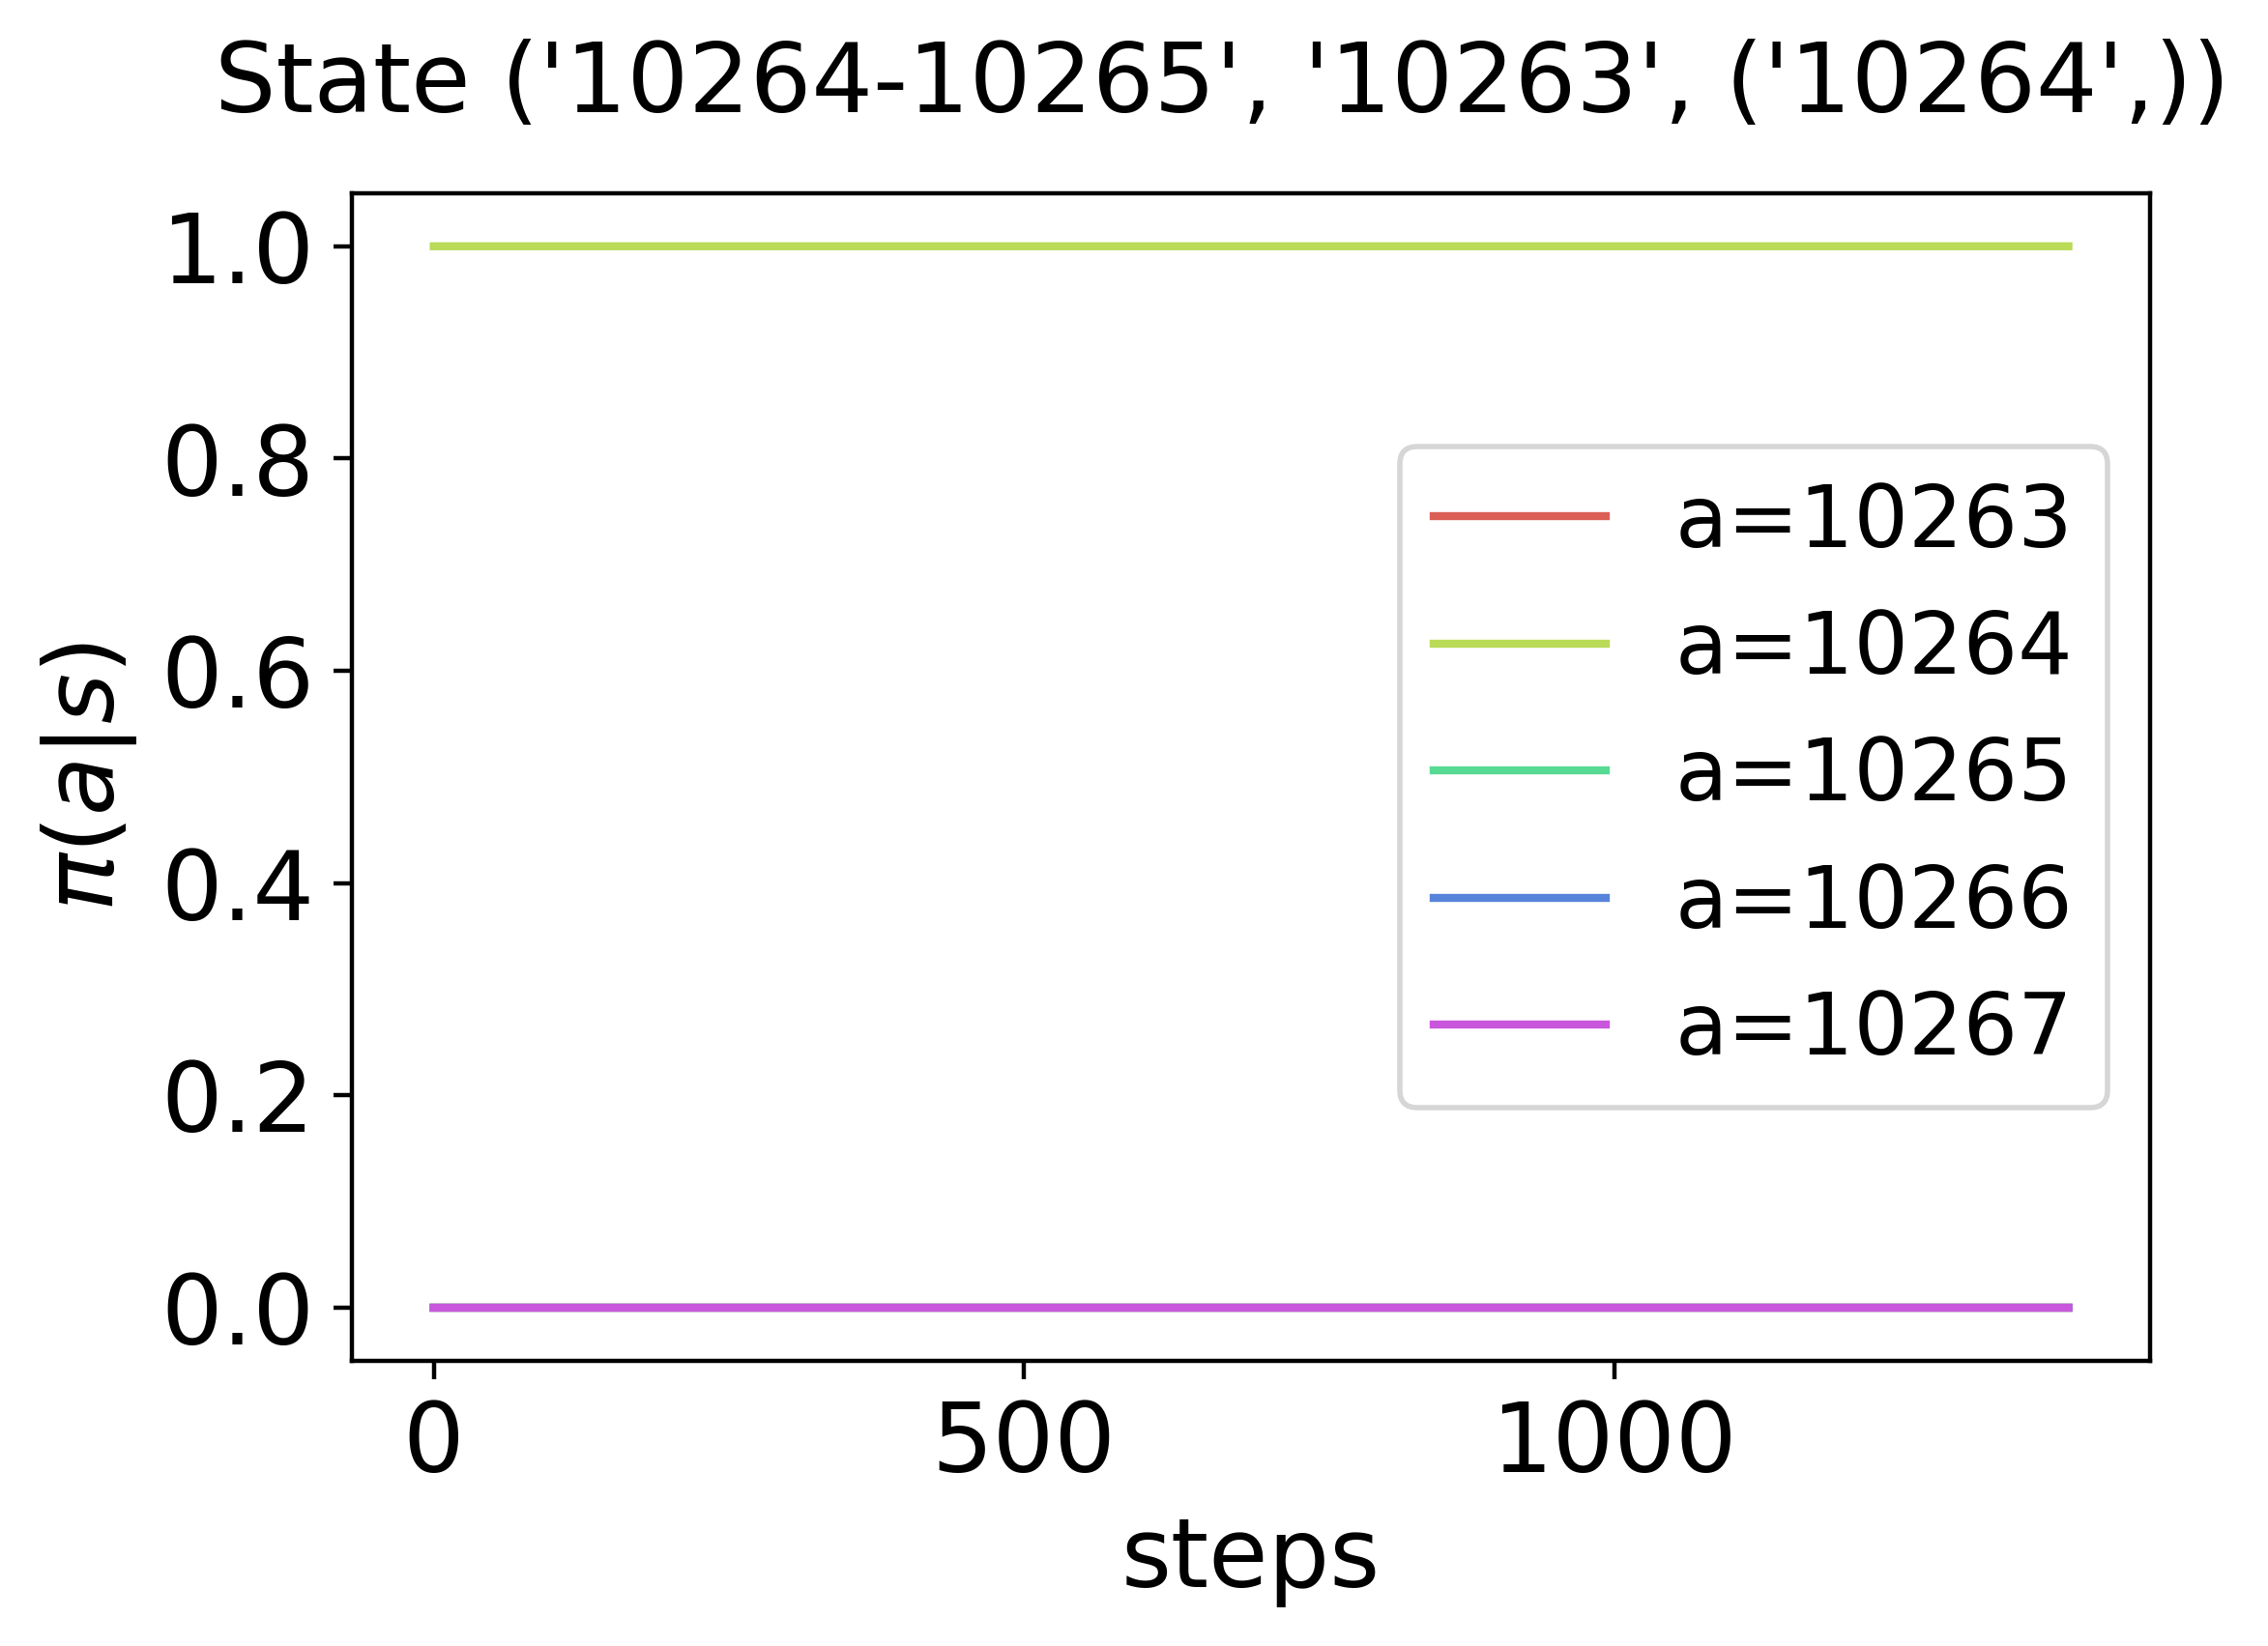
\includegraphics[scale=0.36,valign=b]{chapters/figures/policy_NPG_state_2.png} &
        \hspace*{-18pt}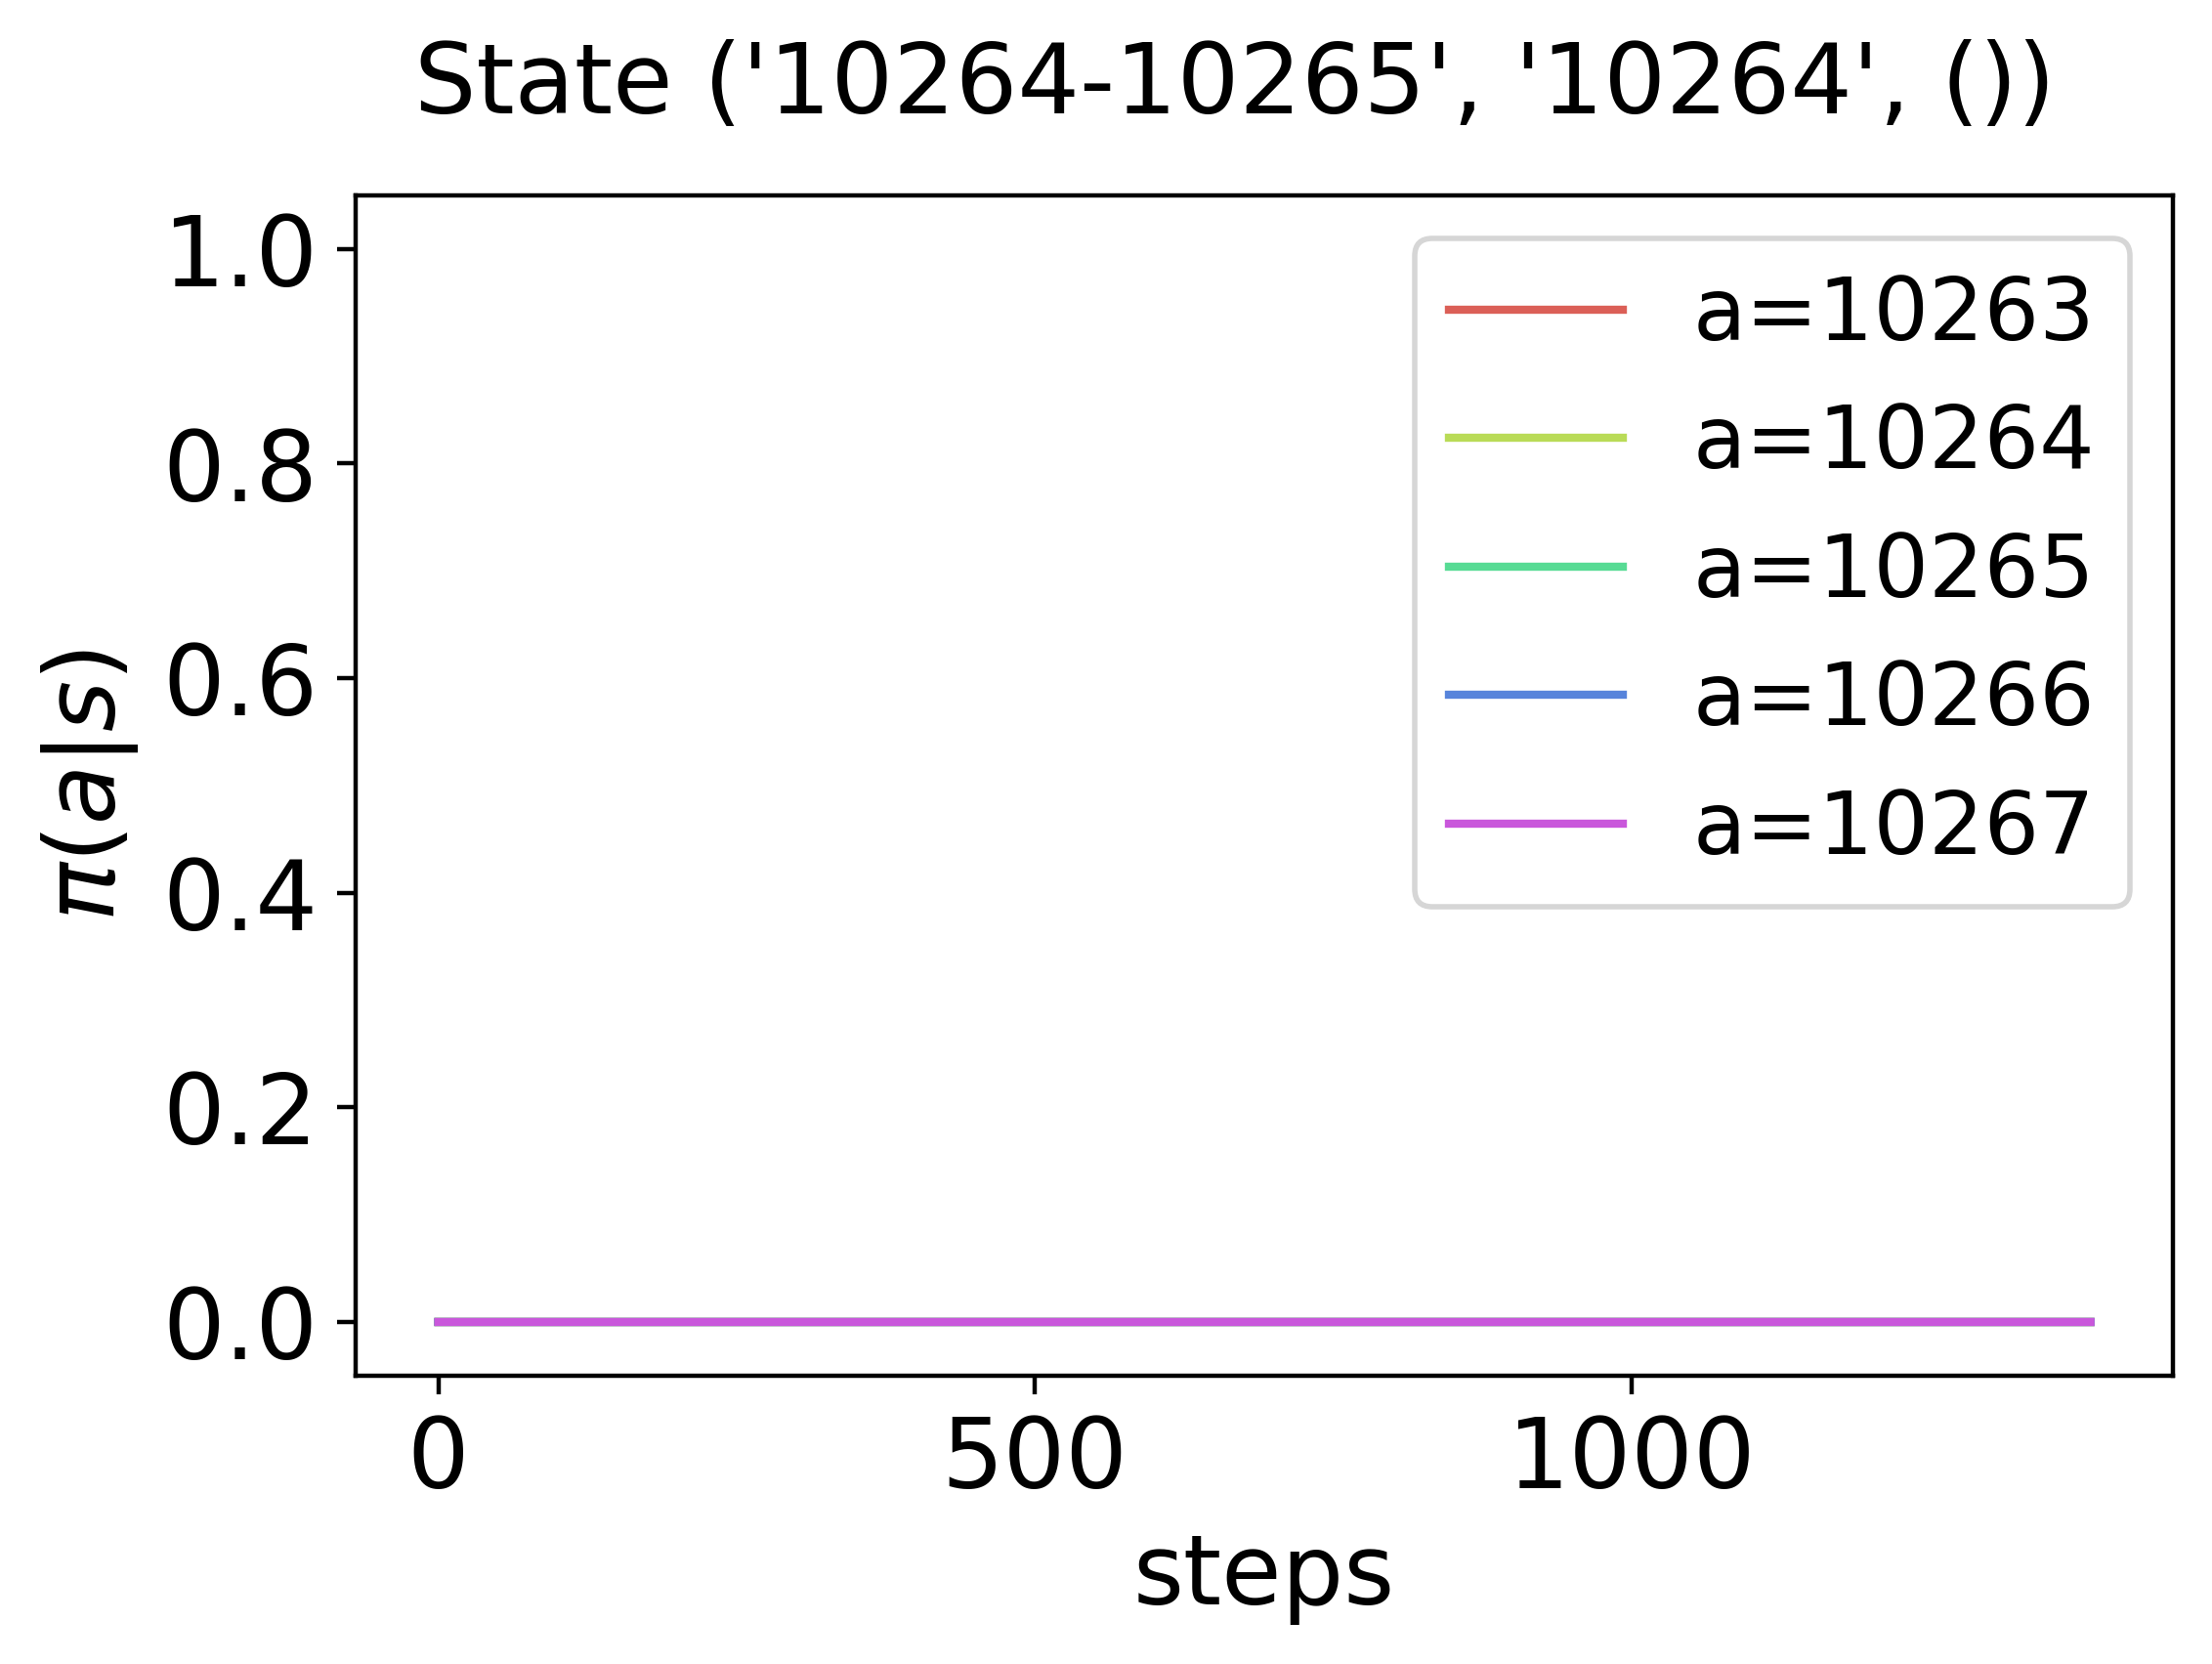
\includegraphics[scale=0.36,valign=b]{chapters/figures/policy_NPG_state_3.png}
    \end{tabular}
    \caption{Trajectories of the policies $\pi_{\boldsymbol \theta}$ in the policy space for \acrshort{npg}, in the exact same previous setting.}
    \label{fig:sequence-policies-npg}
\end{figure}

The most important thing to notice in these figures is that all the trajectories are continuous, without sudden turns backward. Additionally, in the \acrshort{pg} trajectories of $\boldsymbol \theta$ we can see that one of the parameters grows to infinity, while the others either decrease to infinity or are zero (the latter correspond to actions that cannot be taken in that state). In particular, in the last panel all parameters are zero, since in the terminal state we cannot take any action. Moreover, in the second to last panel we have that again all $\theta$s are zero, because we only have one possible action, so the corresponding $\theta$ is zero (in order for the soft-max policy to be equal to $1$), while the others are zero because they correspond to inadmissible actions. Instead, in the \acrshort{npg} we have that all the parameters $\boldsymbol \theta$ decrease, since we are not following the steepest direction in the parameters space, but the steepest direction with respect to the Fisher metric. Even with rather different values of the parameters $\boldsymbol \theta$, the policies are the same (as we already said, when compared among them, the difference is in the order of $10^{-2}$), and from the figures we can see that they reached convergence.

Instead, the standard strategy of checking whether the gradient reached a zero is not applicable in this case: in fact, since we find a stochastic policy, we are not in a corner of the space, in which the gradient is exactly zero, but we are on a side, so it can have values different from zero. Indeed, this is what happens if we look at the gradient matrix: for some states it is not equal to zero, even significantly.

Another check we performed to assess the convergence is to initialize the \acrshort{npg} algorithm with the parameters $\boldsymbol \theta$ found by the \acrshort{pg} algorithm, and vice versa. What we got is that the \acrshort{npg} algorithm continues the gradient descent for about another $600$ steps, reducing a bit the value of $J_\pi(\boldsymbol \theta)$. Actually, the difference is in the order of $10^{-4}$, which is around the $0.001\%$, so it is negligible. Instead, the \acrshort{pg} algorithm exits immediately the gradient descent loop, as soon as the check on the error is performed, and the values of $J_\pi(\boldsymbol \theta)$ are identical (with a difference of $10^{-10}$), as well as the policy (with a difference of $10^{-15}$).

In order to check whether we reached a global minimum or a local one, since we face a non-convex problem, we also performed some random restarts, with the parameters $\boldsymbol \theta$ initialized from a standard normal distribution $\mathcal N(0,1)$. At each run, the algorithm converges to the exact same policy, so we are quite confident that we reached a global minimum. Refs.~\cite{Bhandari2019, bhandari2020note} show that, under some specific conditions, the policy gradient performance measure $J_\pi(\boldsymbol \theta)$ has a unique global minimum, even if it is non-convex. Indeed, they rule out the possibility that the performance measure has another minimum that can be reached from a different initial condition. Given our results, our model could be in this class of problems; however, we did not explore this route, as it was beyond the scope of this thesis.

% Fai i grafi con gli stati con i path di bisezione e di policy gradient (intensità colore in base alla probabilità): così si può vedere che sono diversi.

\section{Performance comparison}

In order to be able to compare all our algorithms together, we compute the performance measure\index{performance measure} $J_\pi(\boldsymbol \theta)$ also for the three bisection algorithms: bisection, bisection improved and weighted bisection. So, first of all, we have to compute the policy matrix of each algorithm. For each state, we find the action that the algorithm would choose in that situation, meaning the substation which it would visit. Then, we encode it in the corresponding policy row as a one hot-vector in which that action has coefficient $1$, while all other actions that can be taken in that state have a $0$, as well as the inadmissible actions. Then we compute the matrix of $Q_\pi$ using equation \eqref{eq:myQ}, in the same way as we did in \autoref{sec:model-implementation}, and we use it to compute the performance measure $J_\pi(\boldsymbol \theta)$ using equation \eqref{eq:myJ}.

\begin{figure}[htb]
    \centering
    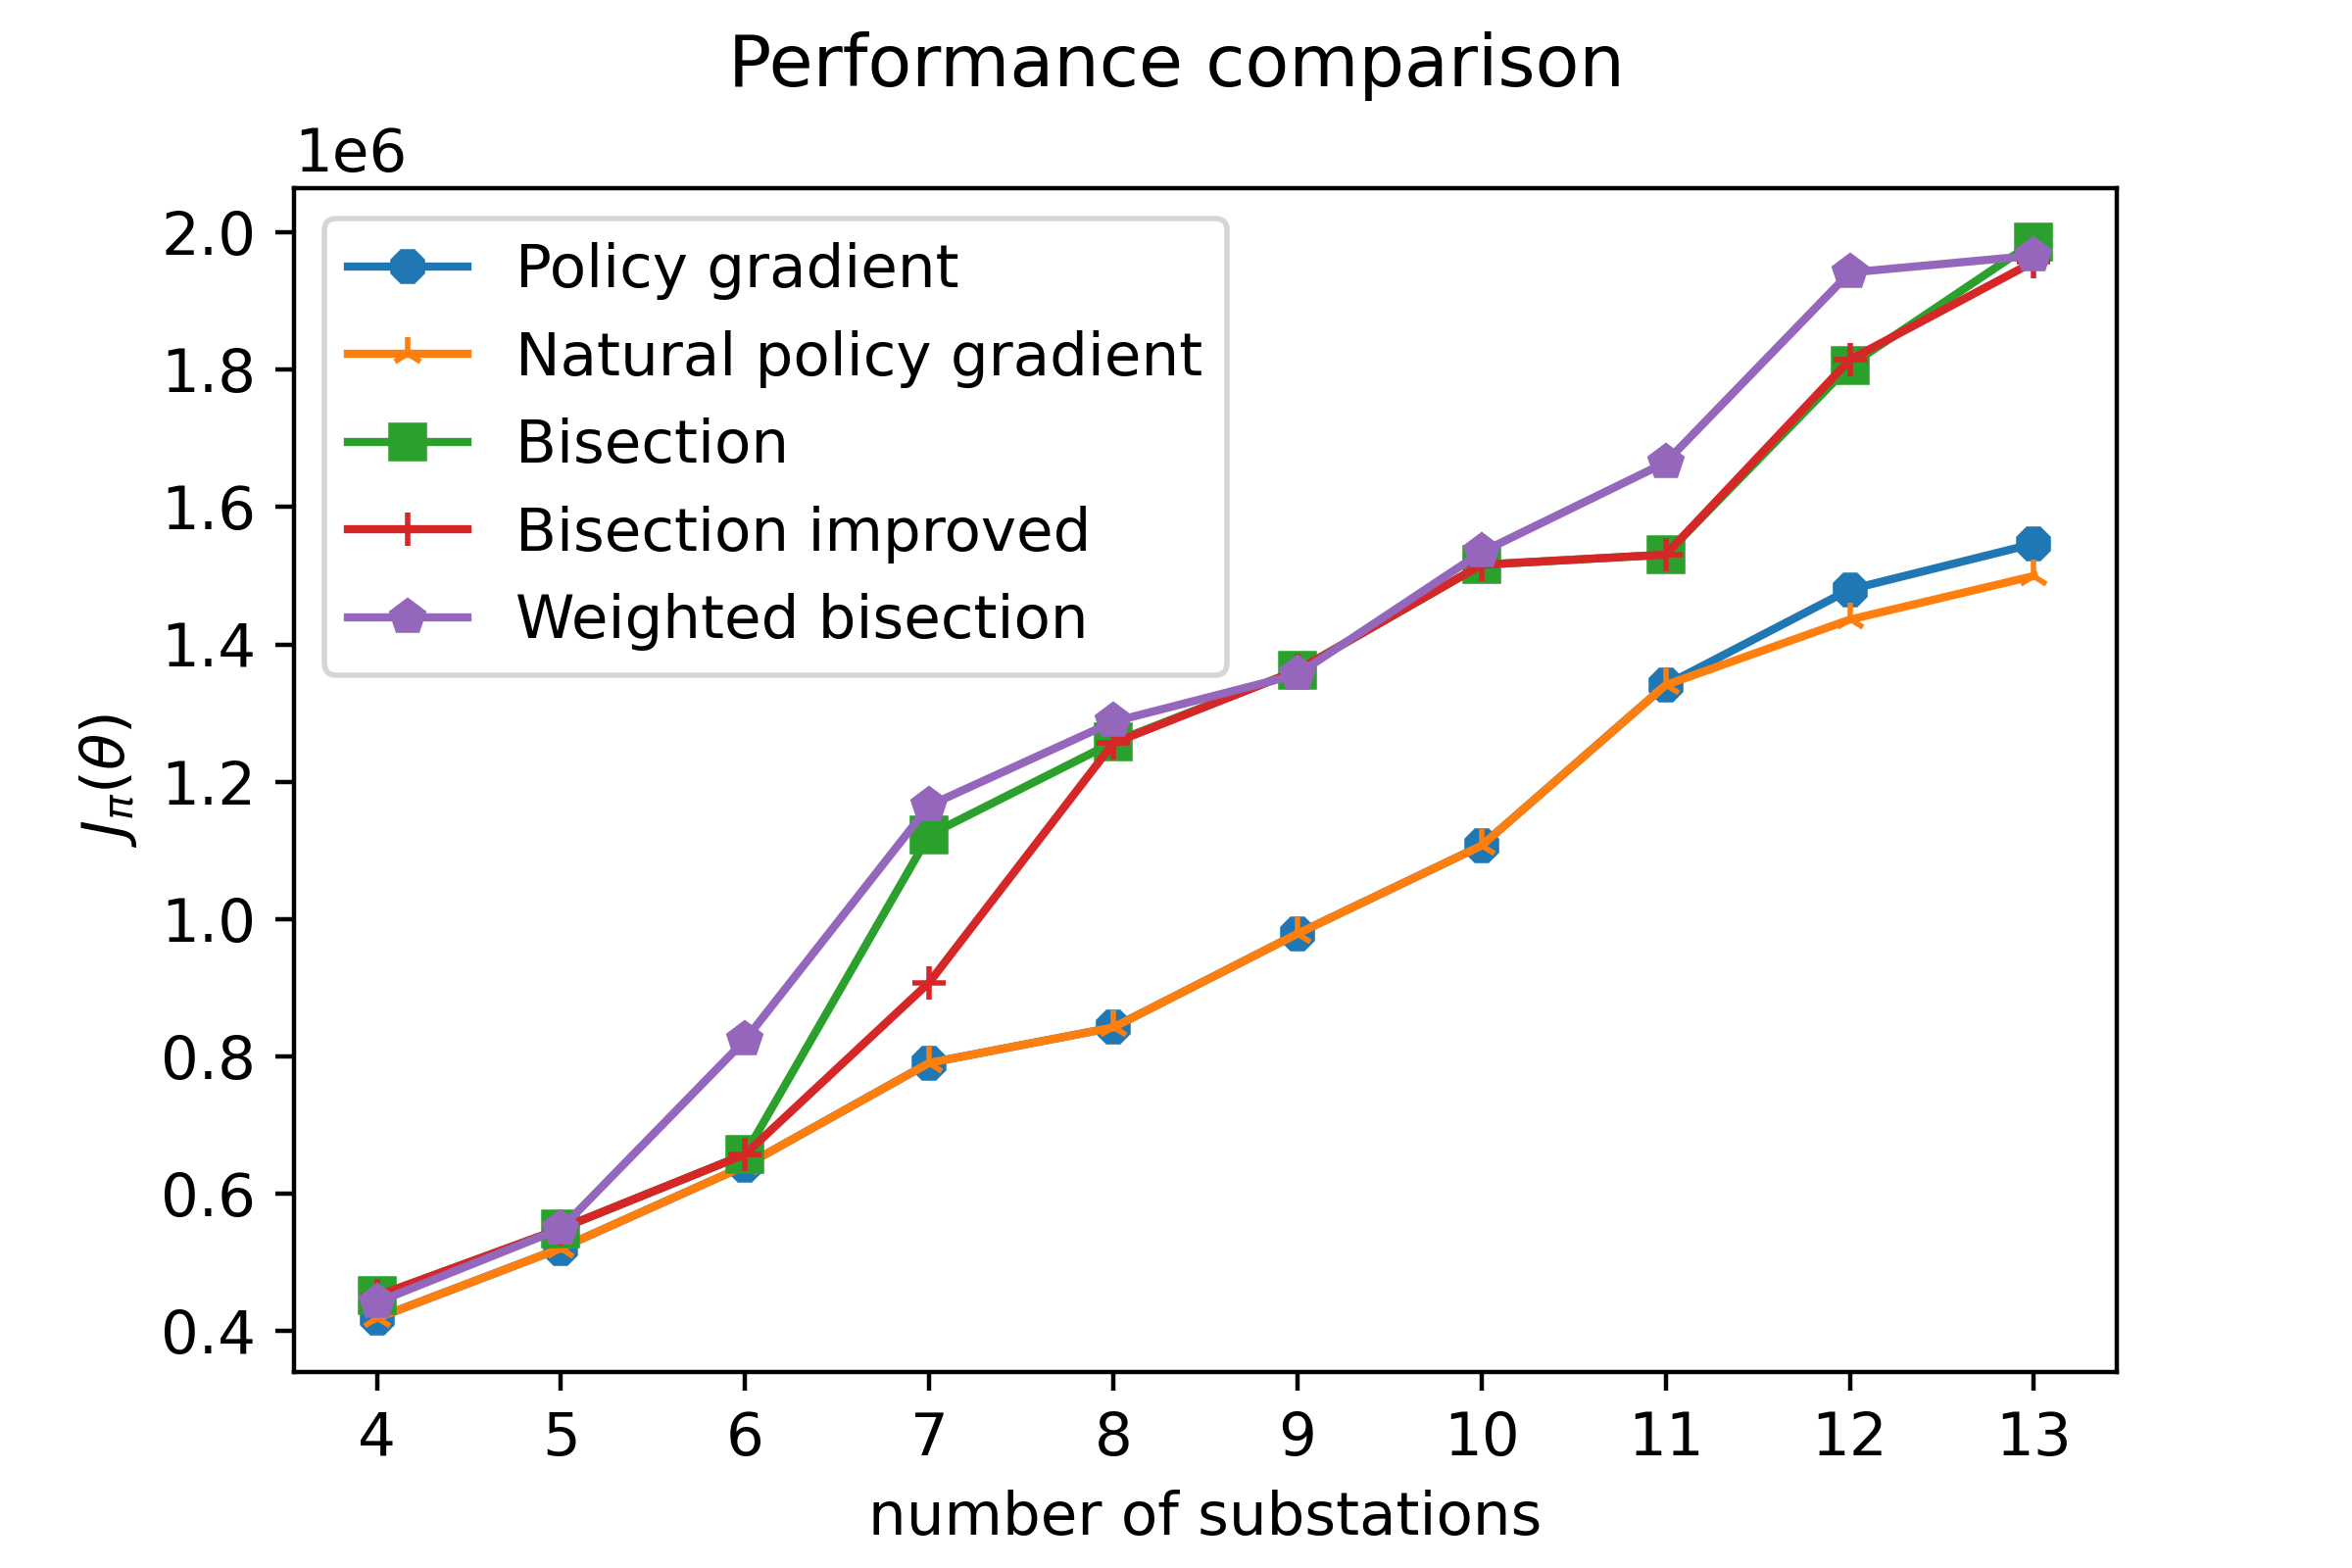
\includegraphics[scale=0.9]{chapters/figures/comparison_graph.png}
    \caption{Comparison of the values of the performance measure $J_\pi (\boldsymbol \theta)$ among the various algorithms for different numbers of initially disconnected substations.}
    \label{fig:comparison-graph}
\end{figure}

Thus, we can compute the exact value of $J_\pi (\boldsymbol \theta)$ for all the algorithms we described, and we can make an effective comparison among all of them. In \autoref{fig:comparison-graph}, we can see the values of $J_\pi(\boldsymbol \theta)$ computed by the various algorithms for different numbers of initially disconnected substations, and for a uniform distribution over the possible positions of the faults. We selected an electrical line of Trieste's power grid, and while keeping the initial position of the technician and the last remotely controlled substation fixed, we fictitiously moved the first remotely controlled substation by one substation each time, in order to incrementally increase the number of initially disconnected substations by one.
% Anche nel comparison graph bisognerebbe dire che J è calcolato solo per i guasti sui cavi
We can clearly see that the policy gradient algorithms are, on average, the better ones, with the \acrshort{npg} a little better with higher numbers of disconnected substations. Instead, the different bisection algorithms perform almost the same, with the weighted bisection a bit worse than the others.

\begin{figure}[htb]
    \centering
    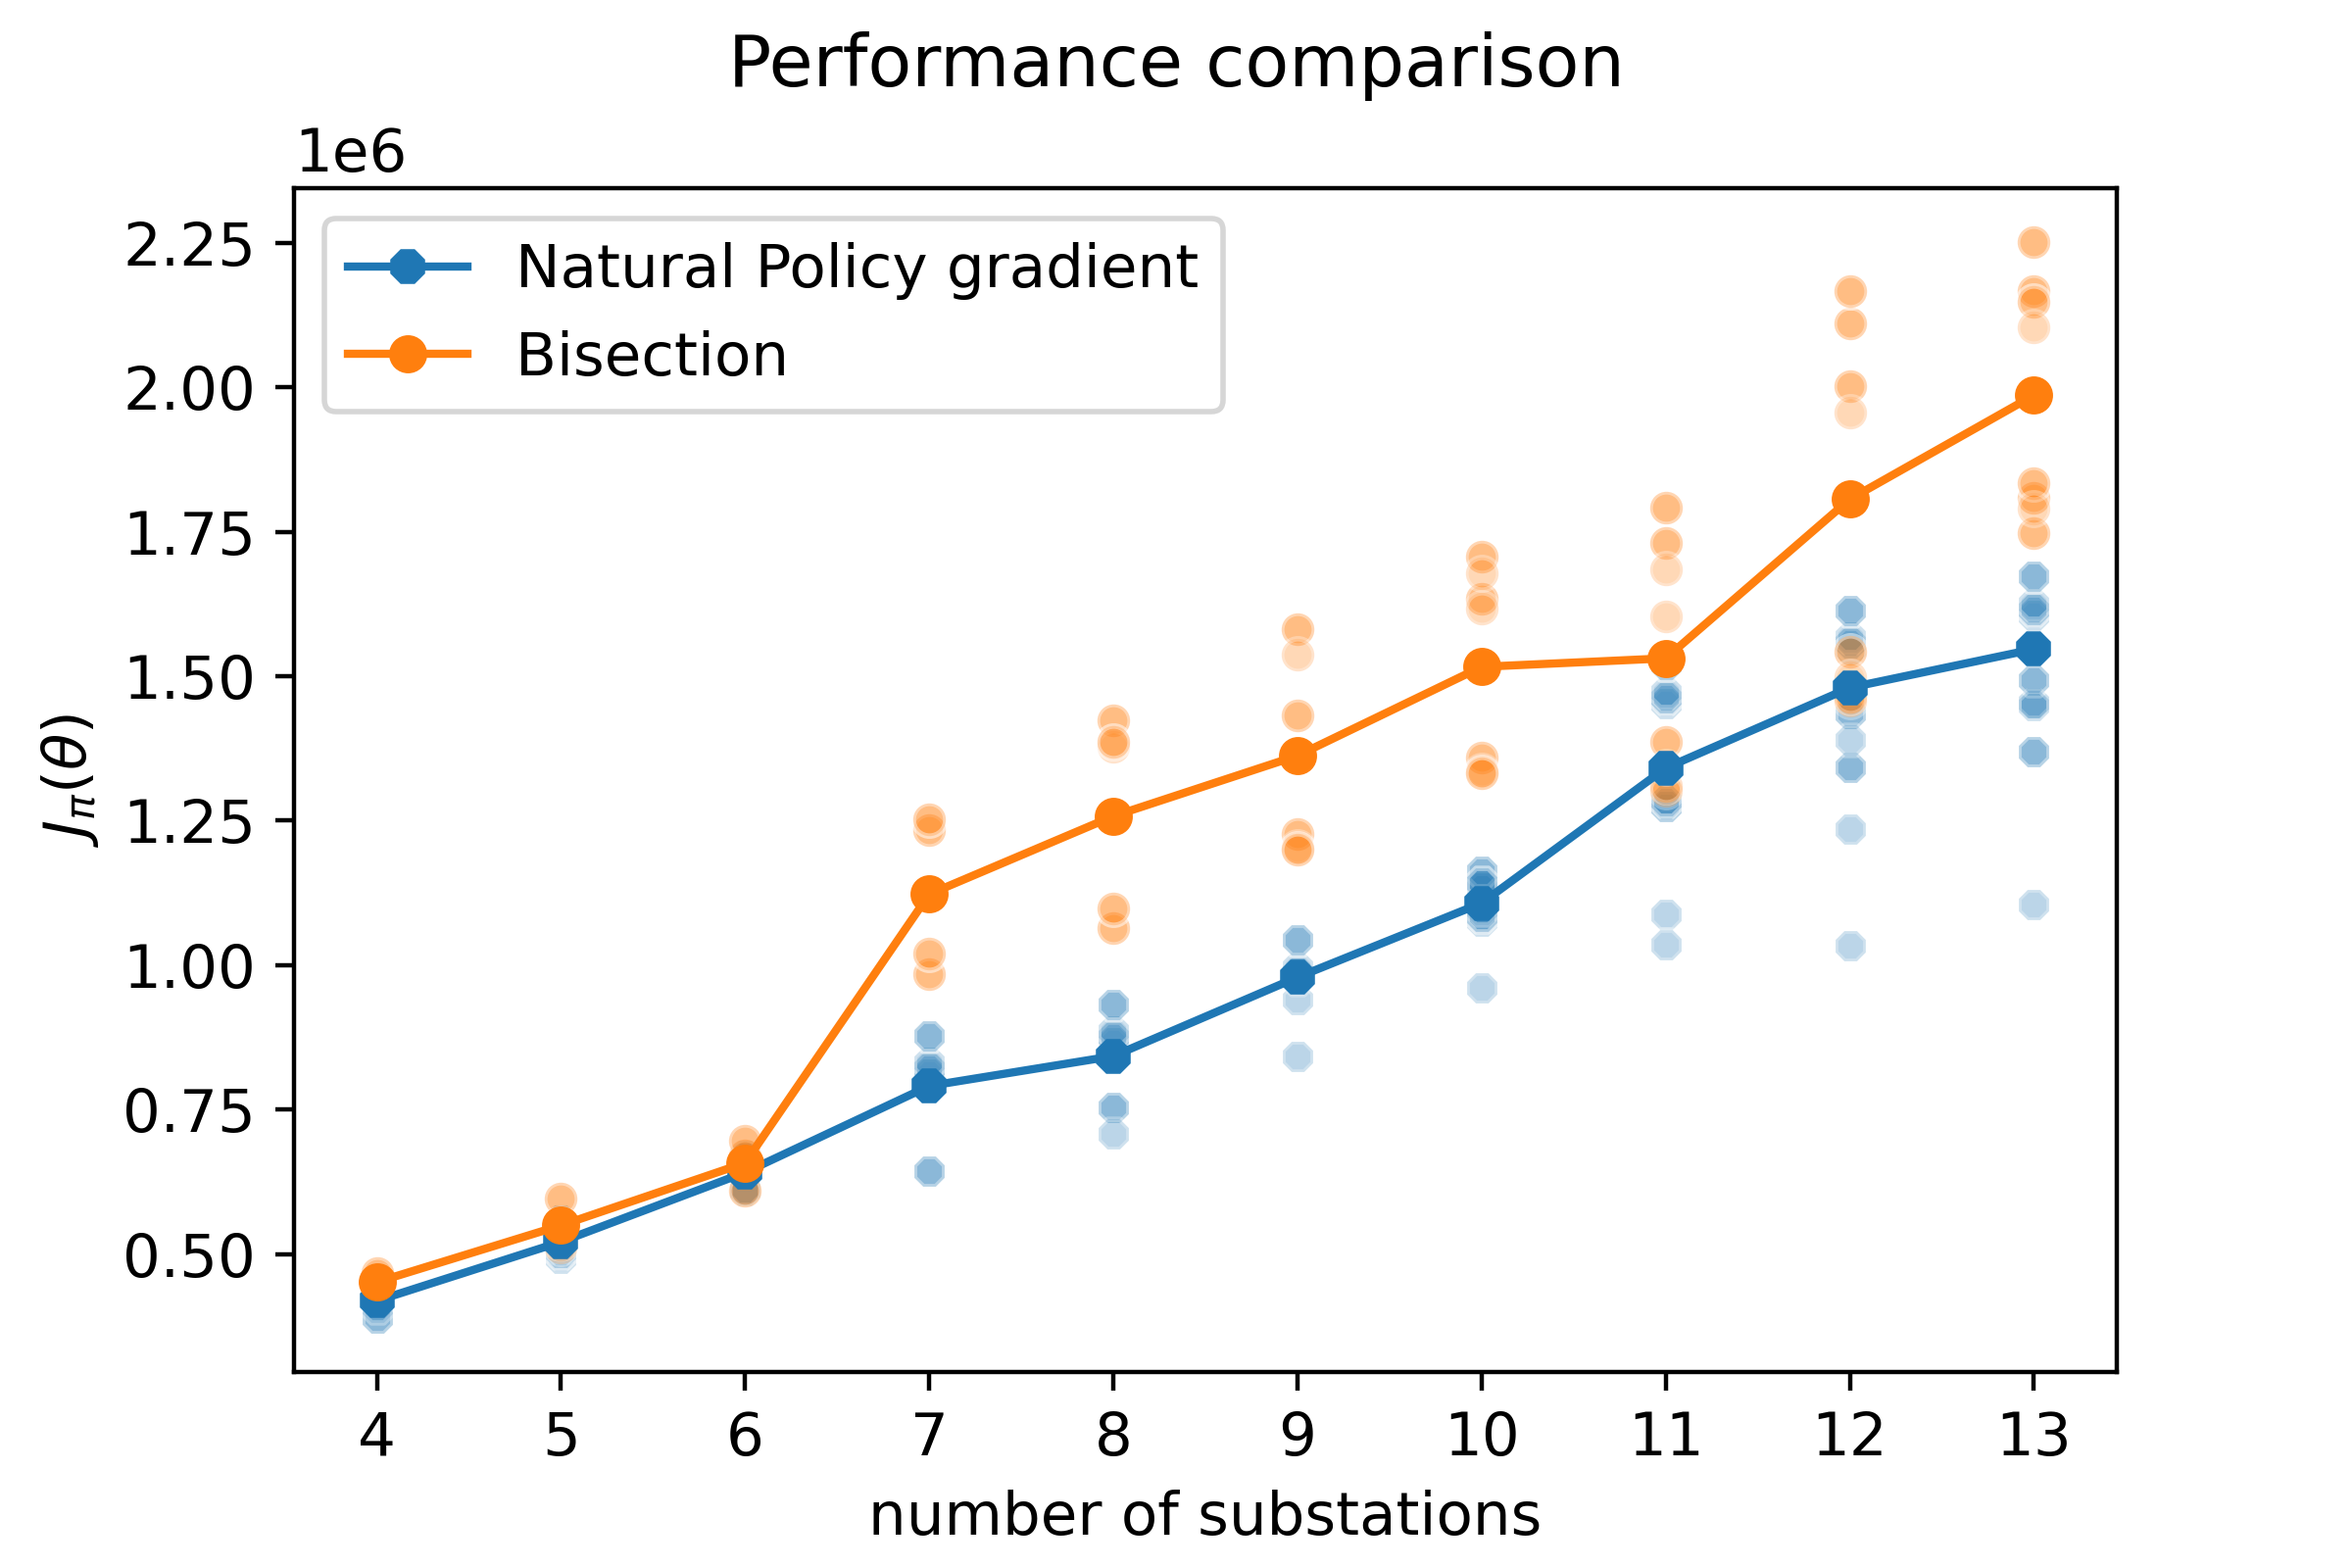
\includegraphics[scale=0.9]{chapters/figures/comparison_graph_scatterplot.png}
    \caption{Comparison of the values of the performance measure $J_\pi (\boldsymbol \theta)$ between \acrshort{npg} and bisection (darker dots), along with the values for every specific position of the fault (lighter dots), for different numbers of initially disconnected substations.}
    \label{fig:comparison-scatterplot}
\end{figure}

\begin{figure}[htb]
    \centering
    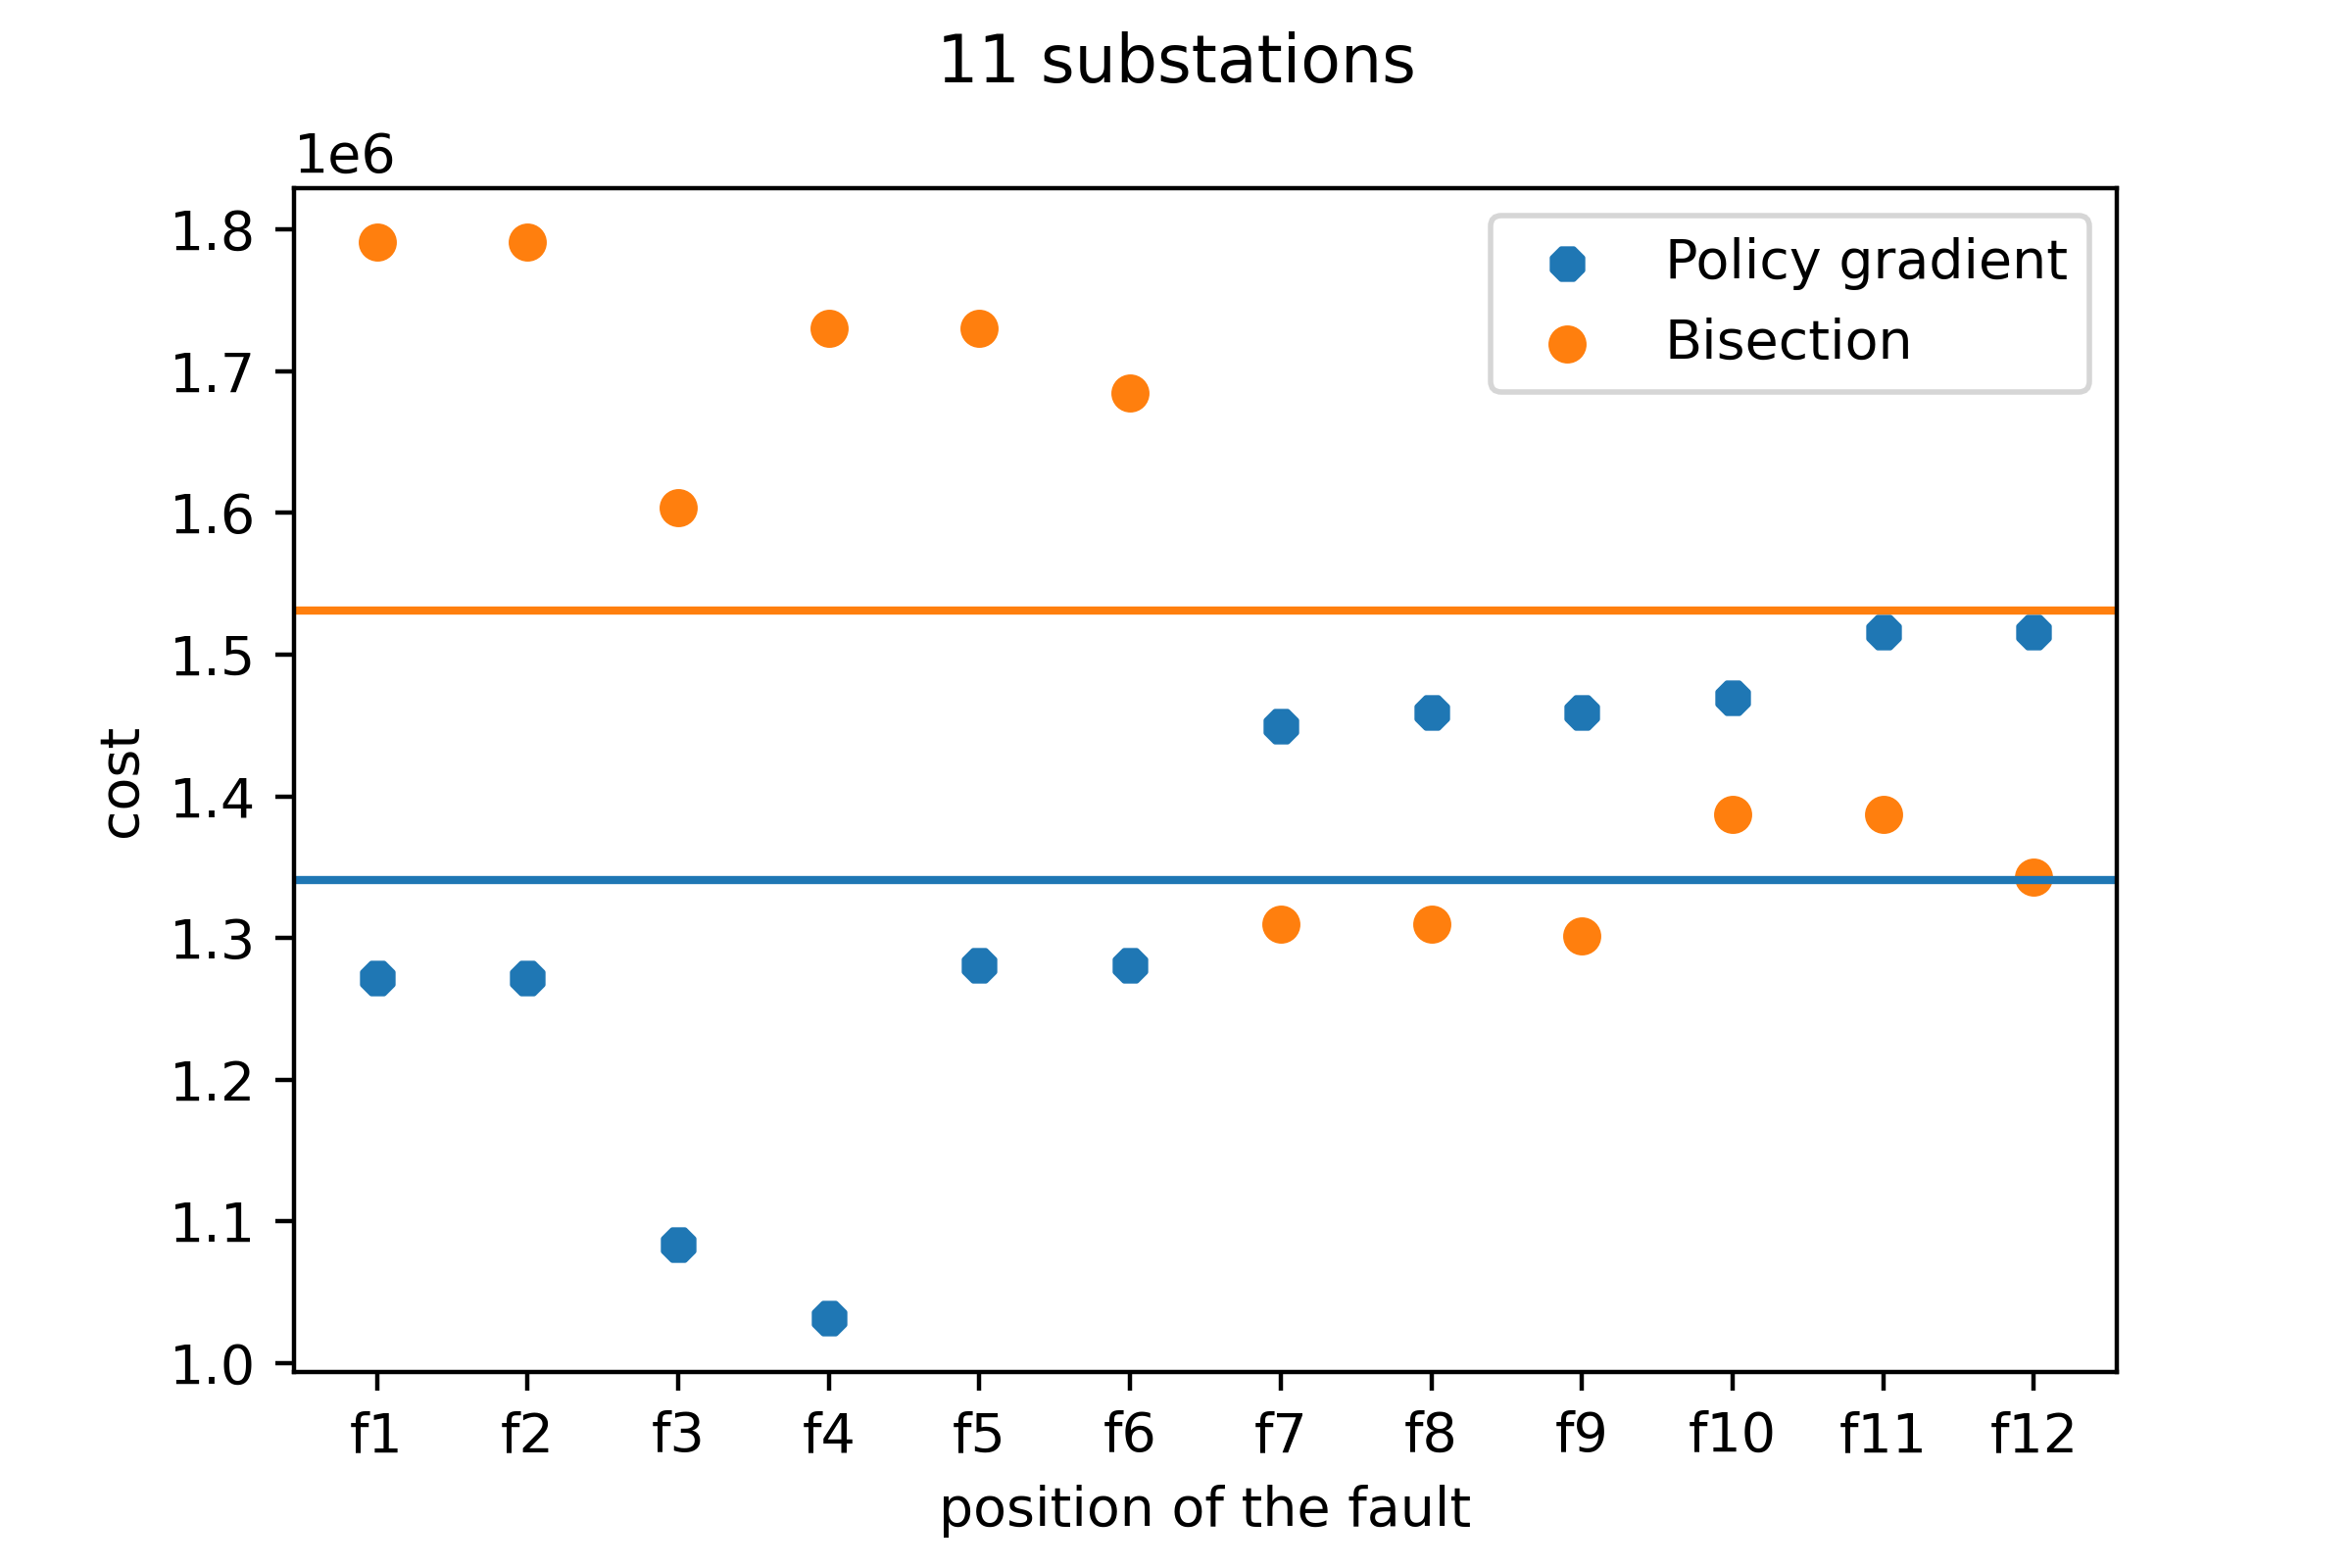
\includegraphics[scale=0.9]{chapters/figures/scatterplot.png}
    \caption{Costs for different positions of the fault in a scenario having $11$ initially disconnected substations. The horizontal lines represent the average cost.}
    \label{fig:scatterplot}
\end{figure}

In \autoref{fig:comparison-scatterplot} we can see the two lines of the \acrshort{npg} and bisection algorithms for $J_\pi(\boldsymbol \theta)$ of the previous plot (the darker dots), with an addition. In fact, we also plotted the performance measure $J_\pi(\boldsymbol \theta)$ computed for each specific position of the fault, meaning that we allowed $x_g$ to take only one specific position at a time, and we iterated over every possible value of that variable and over different numbers of initially disconnected substations (the lighter dots). Since there is the stochastic component of the location of the fault, the actual cost of the fault can vary with respect to the average value found by $J_\pi(\boldsymbol \theta)$, being higher or lower depending on the case.
We considered only the faults on the electrical cables, otherwise there would have been too many points, and since according to the data collected by the technicians they are the most frequent ones, they are the most representative.
We can see that, with $11$ and $12$ initially disconnected substations, for some positions of the fault, the bisection algorithm is actually a slightly better than the \acrshort{npg} one, as some orange points are under some blue points. This is due to the fact that the position of the fault is uncertain, so there is some probability that the bisection algorithm, for a specific position of the fault, chooses a sequence of actions that is better than the one chosen by the \acrshort{npg}. However, the \acrshort{npg} is optimized to perform a lot better on average. We notice a slight overlap with $5$ and $6$ substations as well, but it is not particularly significant.
Instead, for the other numbers of initially disconnected substations, the policy gradient is always better than the bisection. In any case, what is important is that \emph{on average} the \acrshort{npg} is always better, as the value of $J_\pi(\boldsymbol \theta)$ is lower, which was our goal.


% Let's see what happens for each possible position of the fault.

In \autoref{fig:scatterplot} we can see a detail of the previous plot for $11$ initially disconnected substations. We computed the costs of the fault for different positions of the fault of the \acrshort{npg}, the bisection algorithm and a fault specific \acrshort{npg}. The latter is a \acrshort{npg} which was initialized every time with only a specific position for the fault: this means that we modified $\rho_0$ is such a way for it to be a distribution which localizes the fault only on a specific cable. This means that the fault on that specific cable has probability equal to $1$, while all the other possible faults have probability $0$. In this way, the \acrshort{npg} does not have more information than before: the policy still doesn't know where the fault is, but the algorithm can optimize for this specific position of the fault. On the contrary, the bisection algorithm finds a sequence of actions that is completely independent of this a priori knowledge.
So, even here we considered only the faults on the electrical cables, and \texttt{f1} indicates the fault between the first remotely controlled substation and the first disconnected substation, \texttt{f2} indicates the fault between the first and the second disconnected substations, and so on so forth.
%We can see that for some positions of the fault, the bisection algorithm is actually better than the \acrshort{pg} one. But as the value of $J_\pi(\boldsymbol \theta)$, represented by the horizontal lines, is lower in the \acrshort{pg}, we have that on average the latter is better.
We can notice that, if we perform a gradient descent with only a possible position of the fault, the \acrshort{npg} is able to optimize for it, and finds a lower value for the cost than the general \acrshort{npg}.
However, we have to remember that the fault specific \acrshort{npg} is indeed specific for a certain fault, and it has a different policy for every possible position. Thus, it is not applicable in our case, since we don't know where the fault happens, so we cannot choose the appropriate policy that would yield the lower value for the cost.
%In any case, even a fault specific \acrshort{npg} would perform worse than visiting the two exact substations at the ends of the faulty cable, because the policy doesn't know where the fault is.
%It is possible to build a policy that depends on the entire state, thus which knows the position of the fault, and, as we already said in \autoref{chap:model}, it would visit the two substations at the ends of the faulty cable, but in our problem it is of no use.
This is why we create a policy that is optimized for every possible position of the fault, which, in any case, on average performs better than all the other algorithms we used.